% ============================================================
% 第15章 Calabi--Yau多様体と弦理論
% ============================================================
\chapter{Calabi--Yau多様体と弦理論}
\label{ch:ch15}

\begin{chapterlead}
代数幾何・複素幾何の知識が弦理論においてどのように使われるかを理解する、本ノートの中心的応用章。
これまでに学んだ射影多様体・層・因子・複素多様体・ベクトル束と接続の言葉をすべて動員して、
超弦理論の余剰次元の候補である Calabi--Yau 多様体を定義し、具体的に構成し、その Hodge 数を計算する。
章の前半（15.1〜15.4節）では K\"ahler 幾何と Chern 類を整理して Calabi--Yau 多様体の諸定義とその関係を明らかにし、
後半（15.5〜15.7節）では射影空間・重み付き射影空間の超曲面や完全交差として Calabi--Yau 多様体を作る方法と、
特異点とその解消を扱う。最後の15.8節では、10次元超弦理論を Calabi--Yau 多様体上でコンパクト化すると
4次元の超対称理論が得られ、Hodge 数が素粒子の世代数やモジュライ場の数を決めることを見る。
\end{chapterlead}

本章を通じて次の記法を用いる。$X$ は複素次元 $n$ の複素多様体（Calabi--Yau 3-fold なら $n=3$）、
$T_X = T^{1,0}X$ は正則接束、$T^*_X$ はその双対（正則余接束）、
$K_X = \Lambda^n T^*_X$ は標準束（canonical bundle）、$h^{p,q}$ は Hodge 数、$\Omega$ は正則体積形式、
$c_1(X) = c_1(T_X) = -c_1(K_X)$ は第一 Chern 類、$\OO(d)$ は射影空間上の次数 $d$ の直線束である。
複素多様体と Riemann 面の基礎は第13章、ベクトル束・接続・Chern 接続の一般論は第14章で扱ったので、
本章ではそれらを Calabi--Yau 多様体に必要な形で手短に復習し、計算に重点を置く。

% ============================================================
\section{複素多様体の幾何学}
% ============================================================

Calabi--Yau 多様体は「複素多様体 + K\"ahler 計量 + 自明な標準束」という三つの構造の組み合わせである。
本節では一つ目の複素多様体の構造と、その上の正則ベクトル束・微分形式について必要事項をまとめる。

\subsection{複素多様体の復習}

複素次元 $n$ の複素多様体とは、座標変換がすべて双正則であるような $\C^n$ への座標近傍系をもつ Hausdorff・第二可算な位相空間であった（定義\ref{def:ch13-cplx-mfd}）。
局所座標を $z^i = x^i + i y^i$ $(i=1,\dots,n)$ と書く。
$X$ は実 $2n$ 次元の $C^\infty$ 多様体でもあり、座標変換の Jacobi 行列は正則性（Cauchy--Riemann 方程式）から
$\det_\R = |\det_\C|^2 > 0$ を満たすので、複素多様体は自動的に向き付け可能である。

第13章で見たように、代表的な例は次のものである。
\begin{itemize}
\item $\C^n$ とその開集合。
\item 複素トーラス $\C^n/\Lambda$（$\Lambda \cong \Z^{2n}$ は格子）。
\item 射影空間 $\PP^n$。同次座標 $[Z_0:\cdots:Z_n]$ に対し $U_i=\{Z_i\neq 0\}$ 上の座標 $z^{(i)}_j = Z_j/Z_i$ を取ると、座標変換は $z^{(j)}_k = z^{(i)}_k / z^{(i)}_j$ で正則。
\item 射影代数多様体のうち非特異なもの（GAGA により、閉複素部分多様体 $\subset\PP^N$ と同じもの、第13章）。
\end{itemize}

\subsection{複素接束}

$X$ を実多様体と見たときの接束 $TX$ の複素化 $TX\otimes\C$ は、局所的に
$\partial/\partial z^i = \frac12(\partial_{x^i} - i\partial_{y^i})$、$\partial/\partial\bar z^{i} = \frac12(\partial_{x^i} + i\partial_{y^i})$
で張られ、
\[
TX\otimes \C = T^{1,0}X \oplus T^{0,1}X,\qquad
T^{1,0}X = \mathrm{span}\Big\{\frac{\partial}{\partial z^i}\Big\},\quad
T^{0,1}X = \mathrm{span}\Big\{\frac{\partial}{\partial \bar z^{i}}\Big\}
\]
と分解する。この分解は座標変換で保たれる：正則な座標変換 $w = w(z)$ のもとで
\[
\frac{\partial}{\partial z^i} = \frac{\partial w^k}{\partial z^i}\frac{\partial}{\partial w^k}
\]
となり $\partial/\partial\bar w$ 成分が現れないからである。
$T_X := T^{1,0}X$ は遷移関数が Jacobi 行列 $(\partial w^k/\partial z^i)$ という\emph{正則}関数の行列で与えられるので、
次の小節の意味で正則ベクトル束になる。これを\textbf{正則接束}という。

実接束上の\textbf{概複素構造} $J : TX\to TX$ は $J\partial_{x^i} = \partial_{y^i}$、$J\partial_{y^i} = -\partial_{x^i}$ で定まり、
$J^2 = -1$ を満たす。$T^{1,0}$、$T^{0,1}$ はそれぞれ $J$ の固有値 $+i$、$-i$ の固有空間である。
実際 $J(\partial_x - i\partial_y) = \partial_y + i\partial_x = i(\partial_x - i\partial_y)$。
実ベクトル束の同型 $TX \cong T^{1,0}X$, $v\mapsto \frac12(v - iJv)$ により、
「実接ベクトル」と「正則接ベクトル」は同一視できる。

\begin{myex}{$\PP^1$ の正則接束}{ch15-TP1}
$\PP^1 = U_0\cup U_1$、$z = Z_1/Z_0$、$w = Z_0/Z_1 = 1/z$ とする。
$\partial_z = \frac{dw}{dz}\partial_w = -\frac{1}{z^2}\partial_w = -w^2\partial_w$。
したがって $T_{\PP^1}$ の局所枠 $e_0 = \partial_z$（$U_0$ 上）と $e_1 = \partial_w$（$U_1$ 上）は $e_0 = -w^2 e_1$ で結ばれる。
一方 $\OO(k)$ の局所枠 $Z_0^k$（$U_0$ 上）、$Z_1^k$（$U_1$ 上）は $Z_0^k = w^k Z_1^k$ で結ばれる。
遷移関数を比較すると（符号 $-1$ は枠の取り替えで吸収できる）$T_{\PP^1}\cong\OO(2)$ である（例\ref{ex:ch14-ts2}と同じ計算）。
大域切断は $(a+bz+cz^2)\partial_z$ の3次元で、これは $\PP^1$ の自己同型群 $\PGL(2,\C)$ の Lie 環の次元 $3$ に一致する。
\end{myex}

\subsection{正則ベクトル束}

\begin{mydef}{正則ベクトル束}{ch15-holvb}
複素多様体 $X$ 上の階数 $r$ の\textbf{正則ベクトル束}とは、複素多様体 $E$ と正則写像 $\pi:E\to X$ の組で、
局所自明化 $\psi_\alpha:\pi^{-1}(U_\alpha)\xrightarrow{\sim} U_\alpha\times\C^r$ が双正則かつファイバーごとに線形であり、
遷移関数 $g_{\alpha\beta} : U_\alpha\cap U_\beta \to \GL(r,\C)$ が正則であるものをいう。
階数 $1$ のものを（正則）\textbf{直線束}という。
\end{mydef}
これは第14章の定義\ref{def:ch14-holvb}（正則な遷移関数をもつ局所自明化を与えた複素ベクトル束）と同じものである。

正則ベクトル束 $E$ の正則切断の層を $\OO(E)$ と書くと、これは階数 $r$ の局所自由 $\OO_X$-加群であり、
逆に局所自由層から正則ベクトル束が復元される（第11章・第14章）。
以下、ベクトル束と局所自由層を区別せずに扱う。
直線束の同型類は群 $\Pic(X) = H^1(X,\OO_X^*)$ をなし、テンソル積が群演算、双対が逆元である。

正則ベクトル束に対しては、$\bar\partial$ 作用素
\[
\bar\partial_E : \mathcal{A}^{0,q}(E)\to\mathcal{A}^{0,q+1}(E)
\]
が well-defined に定まる。正則な遷移関数 $g_{\alpha\beta}$ は $\bar\partial g_{\alpha\beta}=0$ を満たすので、
局所的に $\bar\partial$ を成分ごとに作用させても枠の取り方によらないからである。
これが「正則構造 $=$ $\bar\partial_E^2=0$ を満たす $\bar\partial$ 作用素」という第14章の見方につながる。

\subsection{外積束}

$T^*X\otimes\C = \Lambda^{1,0}\oplus\Lambda^{0,1}$（$dz^i$ と $d\bar z^{i}$ で張られる）から
\[
\Lambda^k(T^*X\otimes\C) = \bigoplus_{p+q=k}\Lambda^{p,q},\qquad
\Lambda^{p,q} = \Lambda^p(\Lambda^{1,0})\otimes\Lambda^q(\Lambda^{0,1})
\]
を得る。$(p,q)$ 形式は局所的に
\[
\alpha = \frac{1}{p!\,q!}\alpha_{i_1\cdots i_p\bar j_1\cdots\bar j_q}\,dz^{i_1}\wedge\cdots\wedge dz^{i_p}\wedge d\bar z^{j_1}\wedge\cdots\wedge d\bar z^{j_q}
\]
と書ける。複素多様体上では外微分が $d = \partial + \bar\partial$ と分解し、
$\partial^2 = \bar\partial^2 = 0$、$\partial\bar\partial = -\bar\partial\partial$ が成り立つ（概複素構造の可積分性）。

特に重要なのは $\Lambda^{n,0} = \Lambda^n T^*_X$ で、これが直線束
\[
K_X := \Lambda^n T^*_X = \det T^*_X
\]
すなわち\textbf{標準束}である。座標変換 $w=w(z)$ のもとで
\[
dw^1\wedge\cdots\wedge dw^n = \det\Big(\frac{\partial w^k}{\partial z^i}\Big)\,dz^1\wedge\cdots\wedge dz^n
\]
なので、$K_X$ の遷移関数は Jacobi 行列式（の逆）で与えられる。

\begin{myex}{$\PP^1$ の標準束}{ch15-KP1}
$w=1/z$ より $dw = -dz/z^2$、すなわち $dz = -w^{-2}dw$。
$U_0$ 上の枠 $dz$ と $U_1$ 上の枠 $dw$ の関係を例\ref{ex:ch15-TP1}と比べると $K_{\PP^1}\cong\OO(-2) = T_{\PP^1}^*$。
$\OO(-2)$ は正則切断を持たない：実際 $f(z)dz$ が $\PP^1$ 全体で正則なら $f(z)dz = -f(1/w)w^{-2}dw$ が $w=0$ で正則、
すなわち $f$ は無限遠で $z^{-2}$ 以上の速さで減衰する整関数なので $f\equiv 0$。
\end{myex}

\subsection{正則微分形式}

\begin{mydef}{正則 $p$ 形式と Dolbeault コホモロジー}{ch15-holform}
$\bar\partial\alpha = 0$ を満たす $(p,0)$ 形式 $\alpha$ を\textbf{正則 $p$ 形式}という。その層を $\Omega^p_X = \OO(\Lambda^pT^*_X)$ と書く。
\textbf{Dolbeault コホモロジー}を
\[
H^{p,q}_{\bar\partial}(X) = \frac{\Ker(\bar\partial : \mathcal A^{p,q}\to\mathcal A^{p,q+1})}{\Img(\bar\partial:\mathcal A^{p,q-1}\to\mathcal A^{p,q})}
\]
で定め、$h^{p,q} = \dim_\C H^{p,q}_{\bar\partial}(X)$ を \textbf{Hodge 数}という。
\end{mydef}

Dolbeault の定理により $H^{p,q}_{\bar\partial}(X)\cong H^q(X,\Omega^p_X)$（層コホモロジー、第11章）であり、
特に $h^{p,0} = \dim H^0(X,\Omega^p_X)$ は大域的正則 $p$ 形式の個数である。
$X$ がコンパクトなら Hodge 数は有限である。

\begin{myex}{正則形式の例}{ch15-holform-ex}
\begin{enumerate}
\item 複素トーラス $X=\C^n/\Lambda$：$dz^{i_1}\wedge\cdots\wedge dz^{i_p}$ は大域的正則形式で、$h^{p,0} = \binom{n}{p}$。
特に $\Omega = dz^1\wedge\cdots\wedge dz^n$ は至る所零にならない正則 $n$ 形式で、$K_X\cong\OO_X$。
\item $\PP^n$：$p\geq 1$ で $h^{p,0}=0$。$n=1$ は例\ref{ex:ch15-KP1}で見た。一般の $n$ では次節以降で $K_{\PP^n}=\OO(-n-1)$ を示す。
\item 種数 $g$ のコンパクト Riemann 面：$h^{1,0} = g$（第13章）。$K_X$ の次数は $2g-2$。
\end{enumerate}
\end{myex}

正則体積形式、すなわち至る所零にならない正則 $n$ 形式 $\Omega$ が存在することは、$K_X$ が自明束 $\OO_X$ と同型であることに他ならない。
これが Calabi--Yau 多様体の「代数的な」定義の核心である。

\exprob{prob:ch15-1-1}
$\PP^n$ の $U_0=\{Z_0\neq0\}$ 上の座標を $z_i = Z_i/Z_0$、$U_1 = \{Z_1\neq 0\}$ 上の座標を $w_i = Z_i/Z_1$（$i\neq1$、ただし $w_0 = Z_0/Z_1$）とする。
$dz_1\wedge\cdots\wedge dz_n$ を $w$ 座標で表し、$dz_1\wedge\cdots\wedge dz_n = \pm w_0^{-(n+1)}\,dw_0\wedge dw_2\wedge\cdots\wedge dw_n$ となること、すなわち $K_{\PP^n}$ の枠の変換係数が $w_0^{-(n+1)}$（の符号倍）であることを確かめよ。$\OO(k)$ の枠の変換 $Z_0^k = w_0^kZ_1^k$ と比較して
$K_{\PP^n}\cong\OO(-n-1)$ を結論せよ。

\exprob{prob:ch15-1-2}
$J$ を概複素構造とする。$v\in TX$ に対し $v^{1,0} = \frac12(v - iJv)$ が $J$ の固有値 $i$ の固有ベクトルであることを示し、
$v = \partial_{x}$ のとき $v^{1,0} = \partial_z$ となることを確かめよ。

% ============================================================
\section{K\"ahler幾何の基礎}
% ============================================================

Calabi--Yau 多様体の二つ目の構造は K\"ahler 計量である。弦理論の観点では、計量は時空の重力場そのものであり、
「Ricci 平坦」は真空 Einstein 方程式に他ならない。本節では K\"ahler 条件を整理する。

\subsection{Hermitian計量}

\begin{mydef}{Hermitian 計量}{ch15-herm}
複素多様体 $X$ 上の Riemann 計量 $g$ が\textbf{Hermitian}であるとは、概複素構造 $J$ を保つ、すなわち
$g(JX,JY) = g(X,Y)$ が任意の実ベクトル場 $X,Y$ に対して成り立つことをいう。
\end{mydef}

$g$ を $\C$-双線形に拡張すると、$J$ 不変性から $g(\partial_i,\partial_j) = g(\partial_{\bar i},\partial_{\bar j}) = 0$ となる
（$g(\partial_i,\partial_j) = g(J\partial_i,J\partial_j) = i^2 g(\partial_i,\partial_j)$）。したがって
\[
g = g_{i\bar j}\,(dz^i\otimes d\bar z^{j} + d\bar z^{j}\otimes dz^i),\qquad g_{i\bar j} := g(\partial_i,\partial_{\bar j}),
\]
であり、$(g_{i\bar j})$ は正定値 Hermite 行列である（$\overline{g_{i\bar j}} = g_{j\bar i}$）。
\begin{note}
平坦な $\C$ では $g = dx^2 + dy^2 = \frac12(dz\otimes d\bar z + d\bar z\otimes dz)$ なので $g_{z\bar z} = \frac12$ である。
物理の文献では $ds^2 = 2g_{i\bar j}dz^idz^{\bar j}$ とも $ds^2 = g_{i\bar j}dz^idz^{\bar j}$ とも書かれ、係数 $2$ の流儀が混在するので注意。
本章では上の式を定義とする。
\end{note}
Hermitian 計量は正則接束 $T_X$ 上の Hermite 内積 $h(\partial_i,\partial_j) = g_{i\bar j}$ を与える。
これが第14章で扱った「正則ベクトル束上の Hermitian 構造」の特別な場合であり、15.3節で Chern 接続を考えるときに用いる。

任意の複素多様体は Hermitian 計量を持つ。実際、任意の Riemann 計量 $g_0$ から $g(X,Y) = g_0(X,Y)+g_0(JX,JY)$ を作ればよい
（あるいは局所的な $\sum dz^i d\bar z^i$ を1の分割で貼り合わせる）。

\subsection{K\"ahler形式}

\begin{mydef}{基本 2 形式（K\"ahler 形式）}{ch15-kform}
Hermitian 計量 $g$ に対し $\omega(X,Y) := g(JX,Y)$ で定まる実 2 形式を\textbf{基本 2 形式}という。成分では
\[
\omega = i\,g_{i\bar j}\,dz^i\wedge d\bar z^{j}
\]
である。$d\omega=0$ のとき $\omega$ を \textbf{K\"ahler 形式}と呼ぶ。
\end{mydef}

\begin{proof}[成分表示の確認]
$\omega(\partial_i,\partial_{\bar j}) = g(J\partial_i,\partial_{\bar j}) = i g_{i\bar j}$、$\omega(\partial_{\bar j},\partial_i) = g(-i\partial_{\bar j},\partial_i) = -ig_{i\bar j}$。
一方 $i g_{k\bar l}dz^k\wedge d\bar z^l$ を $(\partial_i,\partial_{\bar j})$ に作用させると $i g_{i\bar j}$。$\omega$ は $(1,1)$ 型なので一致する。
平坦な $\C$ では $\omega = \frac{i}{2}dz\wedge d\bar z = dx\wedge dy$ となり、標準的な面積形式を与える。
\end{proof}

$\omega$ は実形式である：$\bar\omega = -i\,\overline{g_{i\bar j}}\,d\bar z^i\wedge dz^j = i g_{j\bar i}dz^j\wedge d\bar z^i = \omega$。
また $\omega^n/n!$ は $g$ の Riemann 体積形式に等しい（平坦な場合 $\omega^n/n! = \prod_i dx^i\wedge dy^i$ を確かめればよい）。
したがって $\omega^n \neq 0$ で、$\omega$ は非退化である。

\subsection{K\"ahler条件}

\begin{mythm}{K\"ahler 条件の同値な言い換え}{ch15-kahlercond}
Hermitian 多様体 $(X,g)$ について、次は同値である。
\begin{enumerate}
\item $d\omega = 0$。
\item 局所的に $\partial_k g_{i\bar j} = \partial_i g_{k\bar j}$（およびその複素共役）。
\item 各点の近傍で実関数 $K$（\textbf{K\"ahler ポテンシャル}）が存在して $g_{i\bar j} = \partial_i\partial_{\bar j}K$、すなわち $\omega = i\partial\bar\partial K$。
\item 各点 $p$ で、$g_{i\bar j}(z) = \delta_{ij} + O(|z|^2)$ となる正則座標（正規正則座標）が取れる。
\item Levi-Civita 接続について $\nabla J = 0$。
\item $T_X$ 上の Chern 接続（15.3.4節）と Levi-Civita 接続が一致する。
\end{enumerate}
\end{mythm}

\begin{proof}[証明の概略]
(1)$\Leftrightarrow$(2)：$d\omega = \partial\omega+\bar\partial\omega$ で
$\partial\omega = i\,\partial_k g_{i\bar j}\,dz^k\wedge dz^i\wedge d\bar z^j$ は $k,i$ について反対称化した $\partial_kg_{i\bar j}-\partial_ig_{k\bar j}$ が消えることと同値。$\bar\partial\omega$ はその複素共役。

(3)$\Rightarrow$(1)：$d(i\partial\bar\partial K) = i(\partial+\bar\partial)\partial\bar\partial K = 0$。
(1)$\Rightarrow$(3)：Poincar\'e 補題で局所的に $\omega = d\eta$ と書き、$\eta = \eta^{1,0}+\eta^{0,1}$（$\eta$ は実なので $\eta^{0,1} = \overline{\eta^{1,0}}$）と分解する。
型を比べると $\bar\partial\eta^{0,1} = 0$、よって局所 $\bar\partial$-Poincar\'e 補題（Dolbeault--Grothendieck の補題）で $\eta^{0,1} = \bar\partial f$。
すると $\omega = \partial\eta^{0,1}+\bar\partial\eta^{1,0} = \partial\bar\partial f + \bar\partial\partial\bar f = i\partial\bar\partial\big(2\,\mathrm{Im} f\big)$。
（$\partial\bar\partial(f-\bar f) = \partial\bar\partial(2i\,\mathrm{Im}f)$ を使った。）

(2)$\Rightarrow$(4)：一次変換で $g_{i\bar j}(0) = \delta_{ij}$ とし、$g_{i\bar j} = \delta_{ij} + a_{ik\bar j}z^k + \overline{a_{jk\bar i}}\bar z^k + O(|z|^2)$ と展開する。
(2) より $a_{ik\bar j}$ は $i,k$ について対称なので、新座標 $w^j = z^j + \frac12 a_{ik\bar j}z^iz^k$ で一次の項が消える。
(4)$\Rightarrow$(5)：正規正則座標の原点で Christoffel 記号はすべて零で、$J$ は定数行列なので $\nabla J=0$ が原点で成立。$p$ は任意。
(5)$\Rightarrow$(1)：$\nabla g = 0$ と $\nabla J=0$ から $\nabla\omega = 0$、捩れのない接続について $d\omega$ は $\nabla\omega$ の反対称化なので $d\omega = 0$。
(6) については15.3.4節で、Chern 接続の Christoffel 記号が $\Gamma^k_{ij} = g^{k\bar l}\partial_ig_{j\bar l}$ であり、(2) の下でこれが $i,j$ について対称（すなわち捩れなし）になることから従う。
\end{proof}

K\"ahler 多様体では Christoffel 記号のうち非零なのは $\Gamma^k_{ij} = g^{k\bar l}\partial_i g_{j\bar l}$ とその複素共役 $\Gamma^{\bar k}_{\bar i\bar j}$ のみで、
「混合型」の $\Gamma^k_{i\bar j}$ などはすべて消える。これは物理の計算で頻繁に用いられる。

\subsection{K\"ahler多様体}

\begin{mydef}{K\"ahler 多様体}{ch15-kahler}
K\"ahler 形式を持つ Hermitian 計量（\textbf{K\"ahler 計量}）を備えた複素多様体を \textbf{K\"ahler 多様体}という。
複素多様体 $X$ が K\"ahler 計量を\emph{少なくとも一つ}持つとき、$X$ は K\"ahler 型であるという。
\end{mydef}

コンパクト K\"ahler 多様体 $X$ では $\omega$ は閉形式なので de Rham 類 $[\omega]\in H^2(X,\R)$ を定め、これを \textbf{K\"ahler 類}という。
$\int_X\omega^n = n!\,\mathrm{Vol}(X) > 0$ なので $[\omega]^n\neq 0$、特に $[\omega]^k\neq 0$ $(0\le k\le n)$ から $b_{2k}(X)\geq 1$ である。
K\"ahler 類全体は $H^{1,1}(X)\cap H^2(X,\R)$ の開凸錐（\textbf{K\"ahler 錐}）をなす。
K\"ahler 類の変形は第16章で Calabi--Yau の K\"ahler モジュライとして詳しく扱う。

コンパクト K\"ahler 多様体の最も重要な性質は \textbf{Hodge 分解}である：
\[
H^k(X,\C) \cong \bigoplus_{p+q=k} H^{p,q}(X),\qquad \overline{H^{p,q}} = H^{q,p},
\]
したがって $b_k = \sum_{p+q=k}h^{p,q}$、$h^{p,q} = h^{q,p}$。さらに Hodge $*$ と Serre 双対性から $h^{p,q} = h^{n-p,n-q}$。
これらは K\"ahler 恒等式 $\Delta_d = 2\Delta_{\bar\partial} = 2\Delta_\partial$ から従う（調和形式による証明は標準的な教科書を参照）。
結果として奇数次 Betti 数は偶数である：$b_{2k+1} = 2\sum_{p<q,\,p+q=2k+1}h^{p,q}$。

もう一つ重要なのが \textbf{$\partial\bar\partial$-補題}である：コンパクト K\"ahler 多様体上の $d$-完全な実 $(1,1)$ 形式 $\alpha$ は
大域的な実関数 $f$ を用いて $\alpha = i\partial\bar\partial f$ と書ける。
これは15.4.4節で Yau の定理を Monge--Amp\`ere 方程式に帰着させる際に本質的に用いられる。

\subsection{K\"ahler幾何の例}

\begin{myex}{平坦な例}{ch15-flat}
$\C^n$ の $K = \sum_i |z^i|^2$ は $g_{i\bar j} = \delta_{ij}$、$\omega = i\sum dz^i\wedge d\bar z^i$ を与える（$g_{i\bar j}=\delta_{ij}$ の規格化では $ds^2 = 2\sum|dz^i|^2$ に注意）。
これは格子 $\Lambda$ の並進で不変なので複素トーラス $\C^n/\Lambda$ に K\"ahler 計量を誘導する。
\end{myex}

\begin{myex}{Fubini--Study 計量}{ch15-FS}
$\PP^n$ の $U_0$ 上で $K = \log(1+|z|^2)$、$|z|^2 = \sum_{k=1}^n|z_k|^2$ とおき、
\[
g_{i\bar j} = \partial_i\partial_{\bar j}\log(1+|z|^2) = \frac{\delta_{ij}}{1+|z|^2} - \frac{\bar z_i z_j}{(1+|z|^2)^2}
\]
と定める。$U_0\cap U_1$ 上で $1+|z|^2 = |Z|^2/|Z_0|^2$、$1+|w|^2 = |Z|^2/|Z_1|^2$ なので
\[
\log(1+|z|^2) = \log(1+|w|^2) + \log|Z_1/Z_0|^2 = \log(1+|w|^2) + \log|z_1|^2
\]
で、$\log|z_1|^2$ は正則関数の実部の2倍なので $\partial\bar\partial\log|z_1|^2 = 0$。
したがって $\omega_{FS} = i\partial\bar\partial\log|Z|^2$ は大域的に well-defined な K\"ahler 形式である。
正定値性は原点で $g_{i\bar j}=\delta_{ij}$ であることと $\mathrm{PU}(n+1)$ の推移的作用から従う。
$n=1$ では $g_{z\bar z} = (1+|z|^2)^{-2}$ で、
\[
\int_{\PP^1}\omega_{FS} = \int_\C \frac{i\,dz\wedge d\bar z}{(1+|z|^2)^2} = \int_{\R^2}\frac{2\,dx\,dy}{(1+r^2)^2} = 2\cdot 2\pi\int_0^\infty\frac{r\,dr}{(1+r^2)^2} = 2\pi .
\]
（$i\,dz\wedge d\bar z = 2\,dx\wedge dy$ と $\int_{\R^2}\frac{dxdy}{(1+r^2)^2} = \pi$ を用いた。）
\end{myex}

\begin{myex}{部分多様体と射影多様体}{ch15-sub}
K\"ahler 多様体 $(M,\omega)$ の複素部分多様体 $X\subset M$ には $\omega|_X$ が K\"ahler 形式を誘導する（$d$ は引き戻しと可換で、正定値性も保たれる）。
したがって\emph{非特異射影多様体はすべて K\"ahler} である。
本章で構成する Calabi--Yau 多様体（$\PP^N$ の超曲面・完全交差）はすべてこれに該当する。
\end{myex}

\begin{myex}{K\"ahler でない複素多様体}{ch15-hopf}
Hopf 曲面 $X = (\C^2\setminus\{0\})/\langle z\mapsto 2z\rangle$ は $S^1\times S^3$ に微分同相で、$b_1 = 1$ は奇数。
したがって Hodge 分解と矛盾し、$X$ は K\"ahler 計量を持たない。
\end{myex}

\exprob{prob:ch15-2-1}
K\"ahler ポテンシャル $K$ を $K + f + \bar f$（$f$ は正則関数）に取り替えても計量 $g_{i\bar j}$ は変わらないことを示せ。
これを用いて、$\PP^n$ の Fubini--Study ポテンシャル $\log(1+|z|^2)$ と $\log(1+|w|^2)$ が $U_0\cap U_1$ 上で同じ計量を与えることを再確認せよ。

\exprob{prob:ch15-2-2}
K\"ahler 多様体上で Levi-Civita 接続の Christoffel 記号のうち $\Gamma^k_{ij} = g^{k\bar l}\partial_ig_{j\bar l}$ とその共役以外が零であることを、
Riemann 幾何の公式 $\Gamma^\lambda_{\mu\nu} = \frac12 g^{\lambda\rho}(\partial_\mu g_{\rho\nu}+\partial_\nu g_{\rho\mu}-\partial_\rho g_{\mu\nu})$ と K\"ahler 条件 $\partial_kg_{i\bar j} = \partial_ig_{k\bar j}$ から確かめよ。

% ============================================================
\section{Chern類とCanonical bundle}
% ============================================================

Calabi--Yau 条件は「$c_1(X)=0$」と表現されることが多い。本節では Chern 類を曲率から定義し（Chern--Weil 理論）、
K\"ahler 多様体の Ricci 形式が第一 Chern 類を代表することを計算で示す。

\subsection{複素ベクトル束}

Chern 類は\emph{複素}ベクトル束（遷移関数が $\GL(r,\C)$ に値を取る $C^\infty$ 束）の位相不変量であり、正則構造は必要ない。
ただし正則ベクトル束に Hermitian 計量を入れると標準的な接続（Chern 接続）が定まり、曲率が具体的に計算できる。
複素ベクトル束 $E$ 上の接続 $\nabla$ は、局所枠 $\{e_\alpha\}$ を用いて $\nabla e_\alpha = \theta_\alpha{}^\beta e_\beta$ と書け、
曲率は $\Theta = d\theta - \theta\wedge\theta$（$\nabla^2 e_\alpha = \Theta_\alpha{}^\beta e_\beta$）である。
枠の取り替え $e' = g e$ のもとで $\Theta' = g\Theta g^{-1}$ と共役変換されるので、
$\Tr\Theta$、$\det(1+t\Theta)$ などの不変多項式は大域的な微分形式を定める（第14章のゲージ共変性）。
\begin{note}
本章では添字を行ベクトル的に $\nabla e_\alpha = \theta_\alpha{}^\beta e_\beta$ と書く（Griffiths--Harris の流儀）。
第14章の $De_j = \sum_i e_iA_{ij}$（$D = d+A$、$F = dA+A\wedge A$）とは $\theta = {}^tA$、$\Theta = {}^tF$ の関係にあり、
曲率の公式の符号 $\Theta = d\theta - \theta\wedge\theta$ の違いは転置によるものにすぎない。$\Tr$ や $\det$ は転置で変わらないので、
Chern 類 $c(E) = \det(1+\frac{i}{2\pi}\Theta) = \det(1+\frac{i}{2\pi}F)$ は両章で同じものである。
\end{note}

\subsection{Chern類の概念}

\begin{mydef}{Chern 類（Chern--Weil の定義）}{ch15-chern}
接続 $\nabla$ を持つ階数 $r$ の複素ベクトル束 $E\to X$ に対し、
\[
c(E) = \det\Big(1 + \frac{i}{2\pi}\Theta\Big) = 1 + c_1(E) + c_2(E) + \cdots + c_r(E),\qquad c_k(E)\in H^{2k}(X,\R)
\]
で \textbf{全 Chern 類}を定める。$c_k(E)$ を第 $k$ \textbf{Chern 類}という。
\end{mydef}

Chern--Weil 理論の基本事実は次の二つである：(i) 右辺の各次数成分は閉形式である（Bianchi 恒等式 $D\Theta = 0$ から）。
(ii) そのコホモロジー類は接続の取り方によらない（二つの接続を線分で結び、差が完全形式になることを示す、いわゆる transgression）。
さらに $c_k(E)$ は整数係数コホモロジー $H^{2k}(X,\Z)$ の像に入る。

Chern 類は次の性質で特徴づけられる。
\begin{enumerate}
\item（自然性）$f:Y\to X$ に対し $c(f^*E) = f^*c(E)$。
\item（Whitney 和公式）完全列 $0\to E'\to E\to E''\to 0$ に対し $c(E) = c(E')\,c(E'')$。
\item（正規化）$\PP^n$ 上で $c(\OO(1)) = 1 + H$、$H$ は超平面類（$\int_{\PP^n}H^n = 1$）。
\end{enumerate}
Whitney 和公式と\textbf{分解原理}（形式的に $E = L_1\oplus\cdots\oplus L_r$、$x_i = c_1(L_i)$ と思ってよい）により
\[
c(E) = \prod_{i=1}^r(1+x_i),\quad c_1(E) = \sum_i x_i,\quad c_2(E) = \sum_{i<j}x_ix_j,\quad c_r(E) = \prod_i x_i .
\]
双対については $c_k(E^*) = (-1)^kc_k(E)$、行列式については $c_1(\det E) = c_1(E)$ が成り立つ。
さらに $X$ がコンパクトで $\dim_\C X = n$ のとき、\textbf{Gauss--Bonnet--Chern の定理}
\[
\chi(X) = \int_X c_n(T_X)
\]
が成り立つ。Calabi--Yau 3-fold の Euler 数はこれで計算する。

\subsection{第一Chern類}

第一 Chern 類は $c_1(E) = \big[\frac{i}{2\pi}\Tr\Theta\big]$ で、$\Tr\Theta = \Tr d\theta$ は $\det E$ の曲率に等しい。
直線束 $L$ に対しては、指数層完全列
\[
0\to\Z\to\OO_X\xrightarrow{\exp(2\pi i\,\cdot)}\OO_X^*\to 0
\]
の連結準同型 $\delta : \Pic(X) = H^1(X,\OO_X^*)\to H^2(X,\Z)$ による像として $c_1(L) = \delta(L)$ を定義することもでき、
二つの定義は（実係数で）一致する。$c_1$ はテンソル積について加法的で、$c_1(L\otimes L') = c_1(L)+c_1(L')$、$c_1(L^*) = -c_1(L)$。

\begin{myprop}{Riemann 面上の次数}{ch15-degree}
コンパクト Riemann 面上の直線束 $L$ に対し $\int_X c_1(L) = \deg L$（因子の次数）。
特に $\int_{\PP^1}c_1(\OO(k)) = k$、$\int_{\PP^1} c_1(T_{\PP^1}) = 2 = \chi(\PP^1)$。
\end{myprop}

\begin{proof}[証明の概略]
$L = \OO(D)$、$D = \sum n_p p$ とし、有理型切断 $s$ を取る。$h$ を Hermitian 計量とすると
曲率形式は $\frac{i}{2\pi}\Theta = -\frac{i}{2\pi}\partial\bar\partial\log|s|_h^2$（$s$ の零点・極を除く）。
各点 $p$ の周りの小円板を除いた領域で Stokes の定理を使うと、境界からの寄与が $\frac{1}{2\pi i}\oint d\log z^{n_p} = n_p$ となり
$\int c_1(L) = \sum n_p = \deg D$。$\OO(k)$ の場合は次の小節の具体計算でも確かめる。
\end{proof}

\subsection{Chern類と曲率}

第14章（定理\ref{thm:ch14-chern-conn}）で見たように、Hermitian 計量 $h$ を持つ正則ベクトル束 $(E,h)$ 上には、
(a) $h$ と両立し、(b) $(0,1)$ 部分が $\bar\partial_E$ に一致する接続（\textbf{Chern 接続}）がただ一つ存在する。
本章の記法で計算を繰り返しておく。
正則枠 $\{e_\alpha\}$ で $h_{\alpha\bar\beta} = h(e_\alpha,e_\beta)$ とおく。(b) より接続形式 $\theta$ は $(1,0)$ 型、(a) より
$\partial h_{\alpha\bar\beta} = \theta_\alpha{}^\gamma h_{\gamma\bar\beta}$ となるので、行列として
\[
\theta = \partial h\cdot h^{-1},\qquad \Theta = d\theta - \theta\wedge\theta = \bar\partial\big(\partial h\cdot h^{-1}\big)
\]
を得る（$\partial\theta = -\partial h\wedge\partial(h^{-1}) = \partial h\, h^{-1}\wedge \partial h\,h^{-1} = \theta\wedge\theta$ を用いた）。
曲率は $(1,1)$ 形式であり、トレースを取ると $\Tr(\partial h\cdot h^{-1}) = \partial\log\det h$ より
\begin{equation}\label{eq:ch15-trTheta}
\Tr\Theta = \bar\partial\partial\log\det h = -\partial\bar\partial\log\det h,\qquad
c_1(E) = \Big[-\frac{i}{2\pi}\partial\bar\partial\log\det h\Big].
\end{equation}

\begin{myex}{$\OO(1)$ の曲率}{ch15-O1curv}
$\PP^n$ 上 $\OO(1)$ の切断は線形形式 $\sum a_iZ_i$ である。自然な Hermitian 計量 $|s|^2_h = |s(Z)|^2/|Z|^2$ を入れると、
$U_0$ 上の正則枠 $e = Z_0$ について $h = |Z_0|^2/|Z|^2 = (1+|z|^2)^{-1}$。式 \eqref{eq:ch15-trTheta} より
\[
\frac{i}{2\pi}\Theta = \frac{i}{2\pi}\partial\bar\partial\log(1+|z|^2) = \frac{\omega_{FS}}{2\pi} .
\]
例\ref{ex:ch15-FS}より $\int_{\PP^1}\omega_{FS}/2\pi = 1$ で、$c_1(\OO(1)) = [\omega_{FS}/2\pi] = H$ と正規化が整合する。
$\OO(d) = \OO(1)^{\otimes d}$ なので $c_1(\OO(d)) = dH$。
\end{myex}

次に $E = T_X$、$h = g$（Hermitian 計量）とする。$(X,g)$ が K\"ahler なら定理\ref{thm:ch15-kahlercond}より Chern 接続は Levi-Civita 接続と一致する。
実際 $\theta = \partial g\cdot g^{-1}$ を成分で書くと $\nabla_{\partial_i}\partial_j = \Gamma^k_{ij}\partial_k$、$\Gamma^k_{ij} = g^{k\bar l}\partial_i g_{j\bar l}$ であり、
これは K\"ahler 条件の下で $i,j$ について対称、すなわち捩れがない。計量と両立し捩れのない接続は Levi-Civita 接続に限る。
したがって $T_X$ の Chern 曲率は Riemann 曲率そのものであり、
\[
R_{i\bar j k}{}^{l} = -\partial_{\bar j}\Gamma^l_{ik},\qquad
R_{i\bar j} := R_{i\bar j k}{}^{k} = -\partial_{\bar j}\Gamma^k_{ik} = -\partial_i\partial_{\bar j}\log\det(g_{k\bar l})
\]
となる（$\Gamma^k_{ik} = \partial_i\log\det g$）。$R_{i\bar j}$ は Riemann 幾何の Ricci テンソルの $(1,1)$ 成分に一致し、
K\"ahler 多様体では Ricci テンソルの $(2,0)$、$(0,2)$ 成分は消える。

\begin{mydef}{Ricci 形式}{ch15-ricci}
K\"ahler 多様体の \textbf{Ricci 形式}を
\[
\rho = i R_{i\bar j}\,dz^i\wedge d\bar z^j = -i\partial\bar\partial\log\det(g_{k\bar l})
\]
で定める。これは $\omega$ と同様に実閉 $(1,1)$ 形式で、$\rho(X,Y) = \mathrm{Ric}(JX,Y)$ を満たす。
\end{mydef}

\begin{mythm}{Ricci 形式は第一 Chern 類を代表する}{ch15-ricci-c1}
コンパクト K\"ahler 多様体 $(X,\omega)$ に対し
\[
c_1(X) = \Big[\frac{\rho}{2\pi}\Big]\in H^2(X,\R).
\]
\end{mythm}

\begin{proof}
式 \eqref{eq:ch15-trTheta} を $E = T_X$、$h = g$ に適用すると
$\frac{i}{2\pi}\Tr\Theta = -\frac{i}{2\pi}\partial\bar\partial\log\det g = \frac{\rho}{2\pi}$。
$\det g$ は局所的な量だが、座標変換で $\det g' = |\det J|^{-2}\det g$（$J$ は正則な Jacobi 行列式）と変換し、
$\partial\bar\partial\log|\det J|^2 = 0$ なので $\rho$ は大域的に定義される。これは $\det g$ が $K_X^{-1} = \det T_X$ 上の Hermitian 計量であることの言い換えである。
\end{proof}

\begin{myex}{Fubini--Study 計量の Ricci 形式}{ch15-FSricci}
$\PP^n$ の $U_0$ 上で $g_{i\bar j} = (1+|z|^2)^{-1}\big(\delta_{ij} - \bar z_iz_j/(1+|z|^2)\big)$。
行列 $\delta_{ij} - \bar z_iz_j/(1+|z|^2)$ はランク1摂動で、その行列式は $1 - |z|^2/(1+|z|^2) = (1+|z|^2)^{-1}$。よって
\[
\det g = (1+|z|^2)^{-(n+1)},\qquad
\rho = -i\partial\bar\partial\log(1+|z|^2)^{-(n+1)} = (n+1)\,\omega_{FS}.
\]
すなわち Fubini--Study 計量は Einstein 計量で $\mathrm{Ric} = (n+1)g$。そして
\[
c_1(\PP^n) = (n+1)\Big[\frac{\omega_{FS}}{2\pi}\Big] = (n+1)H .
\]
$n=1$ では $\int_{\PP^1}c_1 = 2 = \chi(S^2)$（Gauss--Bonnet）。これは15.5節で Euler 列から代数的に再導出する。
\end{myex}

\subsection{Canonical bundle}

\begin{mydef}{標準束と標準因子}{ch15-canonical}
$n$ 次元複素多様体 $X$ の\textbf{標準束}を $K_X = \Lambda^nT^*_X = \det T^*_X$ と定める。その正則切断は正則 $n$ 形式、有理型切断は有理型 $n$ 形式であり、
有理型 $n$ 形式 $\eta\neq0$ の因子 $(\eta)$ を\textbf{標準因子}といって $K_X$ と同じ記号で書く。
\end{mydef}

$H^0(X,K_X) = H^{n,0}(X)$ の次元 $p_g = h^{n,0}$ を幾何種数という。Serre 双対性
$H^q(X,\sheaf{E})\cong H^{n-q}(X,\sheaf{E}^*\otimes K_X)^*$ において $K_X$ は「双対化層」の役割を果たす。
代数幾何では $K_X$ は $\Omega^n_X = \Lambda^n\Omega^1_X$ として定義され（$\Omega^1_X$ は K\"ahler 微分の層）、
特異多様体に対しても（正規かつ Gorenstein なら）直線束として意味を持つ。これは15.7節で重要になる。

\begin{myex}{標準束の計算例}{ch15-Kex}
\begin{enumerate}
\item $\C^n$：$K = \OO\cdot dz^1\wedge\cdots\wedge dz^n$ は自明。
\item 複素トーラス：自明（例\ref{ex:ch15-holform-ex}）。
\item $\PP^1$：$K = \OO(-2)$（例\ref{ex:ch15-KP1}）。有理型形式 $dz$ は $z=\infty$ に2位の極を持ち、標準因子は $-2\cdot[\infty]$。
\item 種数 $g$ の曲線：$\deg K_X = 2g-2$。$g=1$（楕円曲線）でちょうど $K_X\cong\OO_X$ となる。これが1次元の Calabi--Yau 多様体である。
\end{enumerate}
\end{myex}

\subsection{第一Chern類とCanonical bundleの関係}

$K_X = \det T^*_X$ なので
\[
c_1(K_X) = c_1(T^*_X) = -c_1(T_X) = -c_1(X).
\]
したがって
\[
K_X\cong\OO_X\ \Longrightarrow\ c_1(X) = 0\in H^2(X,\Z)\ \Longrightarrow\ c_1(X)_\R = 0\in H^2(X,\R).
\]
逆向きの含意は一般には成り立たない。$c_1(K_X)=0\in H^2(X,\Z)$ は $K_X$ が位相的に自明であることを意味するが、
$\Pic(X)$ の中で $c_1$ の核は $\Pic^0(X) = H^1(X,\OO_X)/H^1(X,\Z)$（ヤコビ多様体型の複素トーラス）であり、
$h^{1,0}=h^{0,1}\neq 0$ なら位相的に自明だが正則には非自明な直線束が存在しうる。
また $H^2(X,\Z)$ の捩れ部分は $\R$ 係数に移ると消えるので、$c_1(X)_\R=0$ でも $K_X$ が非自明な捩れ元でありうる。

\begin{myex}{Enriques 曲面}{ch15-enriques}
K3 曲面 $S$（15.4節）上の固定点を持たない正則対合 $\iota$ による商 $Y = S/\iota$ を Enriques 曲面という。
$\iota^*\Omega_S = -\Omega_S$ なので $\Omega_S$ は $Y$ に降りず、$K_Y\not\cong\OO_Y$ だが $K_Y^{\otimes 2}\cong\OO_Y$。
したがって $c_1(Y)$ は $H^2(Y,\Z)$ の位数2の捩れ元で、$c_1(Y)_\R = 0$。
\end{myex}

\begin{myprop}{$c_1=0$ と $K_X$ の自明性}{ch15-c1K}
コンパクト K\"ahler 多様体 $X$ が $H^1(X,\OO_X) = 0$（$h^{0,1}=0$）を満たし、$c_1(X) = 0\in H^2(X,\Z)$ ならば $K_X\cong\OO_X$。
\end{myprop}

\begin{proof}
指数層完全列から $H^1(X,\OO_X)\to H^1(X,\OO_X^*)\xrightarrow{c_1}H^2(X,\Z)$ が完全。左が零なので $c_1$ は単射であり、$c_1(K_X) = 0$ より $K_X$ は自明。
\end{proof}

\exprob{prob:ch15-3-1}
$\PP^1$ 上で $\OO(k)$ に計量 $h = (1+|z|^2)^{-k}$（$U_0$ 上の枠 $Z_0^k$ に関して）を入れたとき、Chern 曲率から $\int_{\PP^1}c_1(\OO(k)) = k$ を直接計算せよ。

\exprob{prob:ch15-3-2}
分解原理を用いて、階数 $r$ の複素ベクトル束 $E$ について $c_1(\det E) = c_1(E)$ および $c_1(E^*) = -c_1(E)$ を示せ。
また $c(T_{\PP^1}) = 1+2H$ と Gauss--Bonnet--Chern の定理から $\chi(\PP^1)=2$ を確かめよ。

% ============================================================
\section{Calabi--Yau多様体}
% ============================================================

いよいよ Calabi--Yau 多様体を定義する。文献により定義の流儀がいくつかあり、それらの関係を正確に理解することが本節の目標である。

\subsection{Calabi--Yau多様体の定義}

\begin{mydef}{Calabi--Yau 多様体}{ch15-cy}
複素次元 $n$ のコンパクト K\"ahler 多様体 $X$ が \textbf{Calabi--Yau 多様体}であるとは、次の条件を満たすことをいう：
\begin{enumerate}
\item[(CY1)] 標準束が自明：$K_X\cong\OO_X$（すなわち至る所零にならない正則 $n$ 形式 $\Omega$ が存在する）。
\item[(CY2)] $0<i<n$ に対し $h^{i,0}(X) = 0$。
\end{enumerate}
(CY1) のみを課したもの（あるいは (CY1') $c_1(X)_\R = 0$ のみを課したもの）を本章では\textbf{広義の Calabi--Yau 多様体}と呼ぶ。
(CY1)(CY2) を満たすものを、強調するときは \textbf{strict Calabi--Yau 多様体}と呼ぶ。
\end{mydef}

低次元の例を挙げる。
\begin{itemize}
\item $n=1$：$K_X\cong\OO_X$ となるコンパクト Riemann 面は楕円曲線 $\C/(\Z+\tau\Z)$ のみ。(CY2) は空条件。
\item $n=2$：(CY1)(CY2) を満たすコンパクト複素曲面を \textbf{K3 曲面}という（$h^{1,0}=0$）。例：$\PP^3$ の4次曲面 $x_0^4+x_1^4+x_2^4+x_3^4=0$。
2次元複素トーラスは (CY1) を満たすが $h^{1,0} = 2$ なので strict ではない。
\item $n=3$：\textbf{Calabi--Yau 3-fold}。例：$\PP^4$ の5次超曲面（quintic）。弦理論で最も重要なのはこの場合である。
\end{itemize}

\subsection{Canonical bundleの自明性}

(CY1) は正則体積形式 $\Omega\in H^0(X,K_X)$、$\Omega(p)\neq0$ $(\forall p)$ の存在と同値である。$\Omega$ は定数倍を除いて一意である：
$\Omega'$ を別の正則 $n$ 形式とすると $\Omega'/\Omega$ はコンパクト多様体上の正則関数だから定数。すなわち $h^{n,0} = 1$。

$\Omega$ を用いると、正則接束と正則形式の間に同型が得られる：
\begin{equation}\label{eq:ch15-TOmega}
T_X\xrightarrow{\ \sim\ }\Lambda^{n-1}T^*_X = \Omega^{n-1}_X,\qquad v\mapsto \iota_v\Omega .
\end{equation}
各点で $\Omega\neq0$ なので、この縮約は線形同型である（$\C^n$ で $\Omega = dz^1\wedge\cdots\wedge dz^n$ として確かめよ）。
したがって $H^q(X,T_X)\cong H^q(X,\Omega^{n-1}_X) = H^{n-1,q}(X)$。$n=3$、$q=1$ とすると
\[
H^1(X,T_X)\cong H^{2,1}(X).
\]
$H^1(X,T_X)$ は複素構造の無限小変形の空間（Kodaira--Spencer 理論、第16章）なので、\emph{Calabi--Yau 3-fold の複素構造モジュライの次元は $h^{2,1}$} である。

Serre 双対性も簡単になる：$K_X\cong\OO_X$ より $H^q(X,\sheaf{E})\cong H^{n-q}(X,\sheaf{E}^*)^*$。特に $h^{0,q} = h^{0,n-q}$。

\subsection{Holonomyによる定義}

\begin{mydef}{ホロノミー群}{ch15-hol}
Riemann 多様体 $(X,g)$ の点 $p$ において、$p$ を始点・終点とする区分的に滑らかなループに沿った Levi-Civita 接続の平行移動全体がなす群
$\mathrm{Hol}_p(g)\subset O(T_pX)$ を\textbf{ホロノミー群}という。零ホモトープなループに限ったものを\textbf{制限ホロノミー群} $\mathrm{Hol}^0_p(g)$ という。
\end{mydef}

$X$ が連結なら基点によらず共役を除いて定まる。$\mathrm{Hol}^0$ は $\mathrm{Hol}$ の単位元連結成分で、$X$ が単連結なら両者は一致する。
ホロノミーと平行なテンソルの間には次の基本原理がある：\emph{平行（共変定数）なテンソル場は、ホロノミー群で不変な $T_pX$ 上のテンソルと一対一に対応する}。
\begin{itemize}
\item $g$ 自身が平行 $\Rightarrow$ $\mathrm{Hol}\subset O(2n)$。
\item K\"ahler：$J$ が平行（定理\ref{thm:ch15-kahlercond}(5)） $\Leftrightarrow$ $\mathrm{Hol}\subset U(n)$。
\item さらに $\Omega$ が平行 $\Leftrightarrow$ $\mathrm{Hol}\subset SU(n)$。実際 $A\in U(n)$ は $dz^1\wedge\cdots\wedge dz^n$ を $\det A$ 倍するので、これを保つ条件は $\det A = 1$。
\end{itemize}

\begin{mythm}{Ricci 平坦性とホロノミー}{ch15-ricciflat-hol}
$(X,g)$ を K\"ahler 多様体とする。
\begin{enumerate}
\item $g$ が Ricci 平坦 $\Leftrightarrow$ $\mathrm{Hol}^0(g)\subset SU(n)$。
\item $X$ がコンパクトで $K_X\cong\OO_X$、$g$ が Ricci 平坦なら $\Omega$ は平行で、$\mathrm{Hol}(g)\subset SU(n)$。
\end{enumerate}
\end{mythm}

\begin{proof}[証明の概略]
(1) K\"ahler 計量の Levi-Civita 接続は $T_X$ 上の Chern 接続なので、$K_X^{-1} = \det T_X$ に誘導される接続の曲率は $\Tr\Theta = -i\rho$ である。
ホロノミーの $\det$ 部分 $\det:\mathrm{Hol}\to U(1)$ は $K_X^{-1}$ のホロノミーであり、$\rho=0$ ならこの接続は平坦で零ホモトープなループのホロノミーは自明、すなわち $\mathrm{Hol}^0\subset SU(n)$。
逆に $\mathrm{Hol}^0\subset SU(n)$ なら Ambrose--Singer の定理により曲率は $\mathfrak{su}(n)$ に値を取り、トレースが消えて $\rho = 0$。

(2) $|\Omega|^2_g$ を $\Omega\wedge\bar\Omega = c_n\,|\Omega|^2_g\,\omega^n/n!$（$c_n$ は定数）で定めると、局所的に $\Omega = f\,dz^1\wedge\cdots\wedge dz^n$（$f$ 正則）として
$|\Omega|^2 = |f|^2/\det g$。Ricci 平坦なら $\log\det g$ は多重調和なので $\log|\Omega|^2 = \log|f|^2 - \log\det g$ も多重調和、
コンパクト多様体上の多重調和関数は（最大値原理で）定数。よって $|\Omega|$ は定数。
さらに Bochner の公式 $\Delta|\Omega|^2 = 2|\nabla\Omega|^2$（Ricci 平坦で $\Omega$ が正則のとき）から $\nabla\Omega = 0$。
平行な $\Omega$ をホロノミーが保つので $\mathrm{Hol}\subset SU(n)$。
\end{proof}

逆に $\mathrm{Hol}(g)\subset SU(n)$ のコンパクト Riemann 多様体は、平行な $J$ と平行な $\Omega$ を持つので、Ricci 平坦 K\"ahler で $K_X\cong\OO_X$ である。
ホロノミーがちょうど $SU(n)$ であることと (CY2) の関係は次のとおり（Bochner の議論：Ricci 平坦コンパクト多様体上の正則形式はすべて平行）。

\begin{myprop}{ホロノミーと Hodge 数}{ch15-hol-hodge}
$(X,g)$ を $n\geq 2$ 次元のコンパクト Ricci 平坦 K\"ahler 多様体とする。
\begin{enumerate}
\item 正則 $p$ 形式はすべて平行である。したがって $h^{p,0}$ は $\Lambda^p(\C^n)^*$ の中の $\mathrm{Hol}$ 不変元の次元に等しい。
\item $\mathrm{Hol}(g) = SU(n)$ ならば $h^{p,0} = 0$ $(0<p<n)$、$h^{n,0}=1$。特に $X$ は strict Calabi--Yau。
\item 逆に $X$ が単連結で strict Calabi--Yau ならば $\mathrm{Hol}(g) = SU(n)$。
\end{enumerate}
\end{myprop}

\begin{proof}[証明の概略]
(1) Bochner 型の公式により、Ricci 平坦なら正則形式 $\alpha$ について $\Delta|\alpha|^2 = 2|\nabla\alpha|^2\ge0$ で、積分すると $\nabla\alpha = 0$。
(2) $SU(n)$ は $\Lambda^p\C^n$（$0<p<n$）に既約かつ非自明に作用するので不変元は零。$\Lambda^n\C^n$ は $\det$ 表現で $SU(n)$ に対して自明。
(3) Cheeger--Gromoll の分解定理と Berger のホロノミー分類（下の Beauville--Bogomolov 分解）により、単連結なら $X$ は $SU(m)$ ホロノミー多様体と $Sp(m)$ ホロノミー多様体の積に分解する。
$Sp(m)$ 因子は平行な正則 2 形式を、各因子は自身の体積形式を与え、それを引き戻すと $h^{p,0}\neq0$（$p$ は因子の次元）となるので、(CY2) は因子が一つで $SU(n)$ であることを強制する。
\end{proof}

\subsection{Ricci-flat K\"ahler計量}

(CY1) と Ricci 平坦計量を結ぶのが Calabi 予想とその Yau による解決である。

\begin{mythm}{Calabi 予想（Yau の定理）}{ch15-yau}
$X$ をコンパクト K\"ahler 多様体、$\omega$ をその K\"ahler 形式とする。$2\pi c_1(X)$ を代表する任意の実閉 $(1,1)$ 形式 $\rho'$ に対し、
$[\omega'] = [\omega]$ を満たす K\"ahler 形式 $\omega'$ で、その Ricci 形式が $\rho'$ に等しいものがただ一つ存在する。

特に $c_1(X)_\R = 0$ ならば、\emph{各 K\"ahler 類の中に Ricci 平坦 K\"ahler 計量がただ一つ存在する}。
\end{mythm}

\begin{proof}[Monge--Amp\`ere 方程式への帰着]
$c_1(X)_\R=0$ の場合を説明する。$[\rho(\omega)] = 2\pi c_1(X) = 0$ なので $\partial\bar\partial$-補題により $\rho(\omega) = i\partial\bar\partial f$ となる実関数 $f$ が存在する。
求める計量を同じ K\"ahler 類の中で $\omega' = \omega + i\partial\bar\partial\varphi$ と書く（再び $\partial\bar\partial$-補題）。Ricci 形式の公式 $\rho = -i\partial\bar\partial\log\det g$ より
\[
\rho(\omega') - \rho(\omega) = -i\partial\bar\partial\log\frac{\omega'^n}{\omega^n}.
\]
$\rho(\omega') = 0$ とするには $-i\partial\bar\partial\log(\omega'^n/\omega^n) = -i\partial\bar\partial f$、すなわち（コンパクト多様体上の多重調和関数は定数なので）
\[
(\omega + i\partial\bar\partial\varphi)^n = e^{f+c}\,\omega^n,\qquad \omega+i\partial\bar\partial\varphi>0
\]
を解けばよい。定数 $c$ は両辺の積分が一致する条件 $\int_X e^{f+c}\omega^n = \int_X\omega^n$ で決まる。
これは $\varphi$ についての複素 Monge--Amp\`ere 方程式（局所的には $\det(g_{i\bar j}+\partial_i\partial_{\bar j}\varphi) = e^{f+c}\det g_{i\bar j}$）である。
一意性は Calabi による初等的な積分論法、存在は Yau による連続法と $C^0$ 評価を含むアプリオリ評価で示される。
\end{proof}

この定理は\emph{存在定理}であって、コンパクト Calabi--Yau 3-fold の Ricci 平坦計量を閉じた式で書いた例は知られていない。
弦理論の計算で Hodge 数・交点数・周期など「計量によらない」位相的・正則なデータが重視されるのはこのためである。

\begin{mycor}{}{ch15-cy-equiv}
コンパクト K\"ahler 多様体 $X$ について、$c_1(X)_\R = 0$ $\Longleftrightarrow$ $X$ は Ricci 平坦 K\"ahler 計量を持つ $\Longleftrightarrow$ ある K\"ahler 計量について $\mathrm{Hol}^0\subset SU(n)$。
\end{mycor}

\begin{proof}
左から中央は Yau の定理。中央から左は定理\ref{thm:ch15-ricci-c1}で $c_1 = [\rho/2\pi] = 0$。中央と右の同値は定理\ref{thm:ch15-ricciflat-hol}(1)。
\end{proof}

\subsection{定義の違いと数学的注意}

これまでの結果をまとめると、コンパクト K\"ahler 多様体 $X$ に対する条件の間には次の関係がある。
\[
\begin{tikzcd}[row sep=large]
\mathrm{Hol}(g) = SU(n) \arrow[d, Rightarrow, shift right=1.5ex] \\
\text{strict CY: } K_X\cong\OO_X,\ h^{i,0}=0\ (0<i<n) \arrow[u, Rightarrow, shift right=1.5ex, "\pi_1(X)=1"'] \arrow[d, Rightarrow] \\
K_X\cong\OO_X \arrow[d, Rightarrow] \\
c_1(X)_\R = 0 \arrow[d, Leftrightarrow, "\text{Yau}"] \\
\exists\ \text{Ricci 平坦 K\"ahler 計量}\ \Longleftrightarrow\ \mathrm{Hol}^0\subset SU(n)
\end{tikzcd}
\]
注意すべき点を列挙する。
\begin{enumerate}
\item \textbf{$K_X$ 自明 vs $c_1 = 0$}：Enriques 曲面（例\ref{ex:ch15-enriques}）のように $c_1(X)_\R = 0$ でも $K_X$ が非自明なことがある。
ただし Beauville--Bogomolov により $c_1(X)_\R = 0$ なら $K_X$ は捩れ元（ある $m$ で $K_X^{\otimes m}\cong\OO_X$）で、有限被覆を取れば $K_X$ は自明になる。
\item \textbf{$h^{i,0}=0$ 条件の有無}：これを課さないとトーラスや K3$\times T^2$ も含まれる。これらは $\mathrm{Hol}\subsetneq SU(n)$ で、弦理論ではより多くの超対称性を保つ（15.8節）。
\item \textbf{ホロノミー $SU(n)$ と strict CY}：$\mathrm{Hol}=SU(n)$ なら strict CY で $\pi_1(X)$ は有限（$n\ge 3$ のとき）。逆は単連結性を仮定すれば成立する（命題\ref{prop:ch15-hol-hodge}）。
例えば strict CY を自由な有限群作用で割った商は、$\Omega$ が不変なら依然 strict CY だが単連結ではない。
\item \textbf{トーラスと K3}：トーラス $T^{2n}$ は $\mathrm{Hol} = \{1\}$（平坦）。K3 曲面は $SU(2) = Sp(1)$ ホロノミーで、strict CY でありかつ超 K\"ahler でもある。$n = 2$ では SU と Sp の区別がない。
\item \textbf{射影性}：$n\geq3$ の strict CY は $h^{2,0}=0$ なので K\"ahler 錐が $H^2(X,\Q)$ の点を含み、小平の埋め込み定理により射影的である。K3 やトーラスでは一般に射影的でない。
\end{enumerate}

\begin{mythm}{Beauville--Bogomolov 分解}{ch15-BB}
$c_1(X)_\R = 0$ のコンパクト K\"ahler 多様体 $X$ は有限不分岐被覆 $\tilde X\to X$ を持ち、
\[
\tilde X\cong T\times\prod_i Y_i\times\prod_j Z_j
\]
と分解する。ここで $T$ は複素トーラス、$Y_i$ は $\mathrm{Hol}=SU(m_i)$（$m_i\ge3$）の単連結 strict Calabi--Yau、$Z_j$ は $\mathrm{Hol} = Sp(k_j)$ の単連結既約超 K\"ahler 多様体。
\end{mythm}

\begin{physbox}[定義の流儀]
物理の文献で単に「Calabi--Yau 多様体」と言えば、ほとんどの場合 $\mathrm{Hol} = SU(3)$ の Calabi--Yau 3-fold（したがって $h^{1,0} = h^{2,0} = 0$）を指す。
$T^6$ や $K3\times T^2$ 上のコンパクト化は、保たれる超対称性が多すぎて（それぞれ 4次元 $\mathcal N=8$、$\mathcal N=4$（タイプII））現実的な模型の構成には向かないが、
厳密に解ける例として重要である。本章でも以下、特に断らなければ strict Calabi--Yau 3-fold を考える。
\end{physbox}

\subsection{Calabi--Yau多様体の基本的性質}

strict Calabi--Yau 3-fold $X$ の Hodge 数を決めよう。Hodge 対称性 $h^{p,q} = h^{q,p} = h^{3-p,3-q}$ と
\[
h^{0,0} = 1,\quad h^{1,0} = h^{2,0} = 0,\quad h^{3,0} = 1
\]
から、独立な Hodge 数は $h^{1,1}$ と $h^{2,1}$ の二つだけである。実際、例えば $h^{1,0}=0$ から $h^{0,1}=h^{3,2}=h^{2,3}=0$、$h^{2,0}=0$ から $h^{0,2}=h^{3,1}=h^{1,3}=0$ となる。
ダイアモンドは図\ref{fig:ch15-hodge-cy3}の形になる。

\begin{figure}[H]
\centering
\setlength{\arraycolsep}{2.5pt}
\[
\begin{array}{ccccccc}
 & & & h^{3,3} & & & \\
 & & h^{3,2} & & h^{2,3} & & \\
 & h^{3,1} & & h^{2,2} & & h^{1,3} & \\
h^{3,0} & & h^{2,1} & & h^{1,2} & & h^{0,3}\\
 & h^{2,0} & & h^{1,1} & & h^{0,2} & \\
 & & h^{1,0} & & h^{0,1} & & \\
 & & & h^{0,0} & & &
\end{array}
\qquad = \qquad
\begin{array}{ccccccc}
 & & & 1 & & & \\
 & & 0 & & 0 & & \\
 & 0 & & h^{1,1} & & 0 & \\
1 & & h^{2,1} & & h^{2,1} & & 1\\
 & 0 & & h^{1,1} & & 0 & \\
 & & 0 & & 0 & & \\
 & & & 1 & & &
\end{array}
\]
\caption{strict Calabi--Yau 3-fold の Hodge ダイアモンド。$k$ 行目（下から）の和が Betti 数 $b_k$ を与える。}
\label{fig:ch15-hodge-cy3}
\end{figure}

Betti 数は $b_0=b_6=1$、$b_1=b_5=0$、$b_2=b_4=h^{1,1}$、$b_3 = 2+2h^{2,1}$ であり、Euler 数は
\[
\chi(X) = \sum_k(-1)^kb_k = 2 + 2h^{1,1} - (2+2h^{2,1}) = 2\big(h^{1,1}-h^{2,1}\big).
\]

\begin{myprop}{strict Calabi--Yau 多様体の基本性質}{ch15-cy-prop}
$X$ を strict Calabi--Yau $n$-fold（$n\ge 2$）とする。
\begin{enumerate}
\item $\chi(X,\OO_X) = \sum_q(-1)^qh^{0,q} = 1+(-1)^n$。$n=3$ なら $0$。
\item $H^0(X,T_X) = 0$。すなわち $X$ は（連続的な）正則ベクトル場を持たず、$\Aut(X)$ は離散群。
\item $n=3$ のとき $H^1(X,T_X)\cong H^{2,1}(X)$、$H^1(X,T^*_X) = H^{1,1}(X)$。
\item $n\ge3$ なら $H^2(X,\Z)\cong\Pic(X)$（$c_1$ による）。特に $h^{1,1} = \rank\Pic(X) = \rho(X)$（Picard 数）。
\end{enumerate}
\end{myprop}

\begin{proof}
(1) $h^{0,q} = h^{q,0}$ で、これは $q=0,n$ で $1$、それ以外で $0$。
(2) 式\eqref{eq:ch15-TOmega} より $H^0(T_X)\cong H^0(\Omega^{n-1}) $ で、$h^{n-1,0} = 0$。
(3) 同じく $H^1(T_X)\cong H^{n-1,1} = H^{2,1}$。
(4) 指数層完全列 $H^1(\OO_X)\to\Pic(X)\to H^2(X,\Z)\to H^2(\OO_X)$ で、$h^{0,1}=h^{0,2}=0$。
\end{proof}

\exprob{prob:ch15-4-1}
K3 曲面 $S$（$K_S\cong\OO_S$、$h^{1,0}=0$）の Hodge ダイアモンドを求めよ。ただし Noether の公式 $\chi(S,\OO_S) = \frac{1}{12}\int_S(c_1^2+c_2)$ を用いてよい。
（答：$h^{1,1}=20$、$\chi(S)=24$。）

\exprob{prob:ch15-4-2}
$U(n)$ の元 $A$ が $\C^n$ 上の $(n,0)$ 形式 $dz^1\wedge\cdots\wedge dz^n$ を $\det A$ 倍することを示し（$A$ の作用は余接空間への双対作用とする。符号・共役に注意）、
$SU(n)$ が $\Lambda^p(\C^n)^*$（$0<p<n$）に不変な非零元を持たないことを $n=3$, $p=1,2$ の場合に確かめよ。

% ============================================================
\section{Calabi--Yau多様体の具体的構成}
% ============================================================

Yau の定理のおかげで、Calabi--Yau 多様体を作るには Ricci 平坦計量を探す必要はなく、
「$K_X$ が自明なコンパクト K\"ahler 多様体」を作ればよい。これは純粋に代数幾何の問題であり、射影空間の超曲面・完全交差を使うのが最も基本的な方法である。

\subsection{射影空間内の超曲面}

$F\in\C[Z_0,\dots,Z_N]_d$ を $d$ 次斉次多項式とし、
\[
X = \Zero(F) = \{[Z]\in\PP^N\mid F(Z) = 0\}
\]
を考える。$F$ は関数ではないが、$F(\lambda Z) = \lambda^dF(Z)$ なので零点集合は well-defined であり、
$F$ は直線束 $\OO(d)$ の大域切断 $F\in H^0(\PP^N,\OO(d))$ と見なせる。$X$ はその零因子である。

\begin{myprop}{超曲面の非特異性（Jacobi 判定法）}{ch15-jacobi}
$X = \Zero(F)$ が非特異であるための必要十分条件は、$\PP^N$ 上で連立方程式
$\partial F/\partial Z_0 = \cdots = \partial F/\partial Z_N = 0$ が共通零点を持たないことである。
\end{myprop}

\begin{proof}[証明の概略]
Euler の恒等式 $\sum_iZ_i\,\partial F/\partial Z_i = d\cdot F$ により、すべての偏微分が消える点では（$d\neq0$ なので）自動的に $F=0$。
アフィンチャート $Z_0 = 1$ では $f(z) = F(1,z)$ で、点 $p\in X$ が特異 $\Leftrightarrow$ $\partial f/\partial z_i(p) = 0$ $(\forall i)$。
Euler の恒等式を使うと、これは $\partial F/\partial Z_i(p) = 0$ $(\forall i)$ と同値（第7章の Jacobi 判定法）。
\end{proof}

Bertini の定理により、一般の（係数を generic に取った）$F$ に対して $X$ は非特異である。非特異な超曲面は例\ref{ex:ch15-sub}により K\"ahler 多様体であり、
Lefschetz の超平面定理により $N\geq 3$ なら連結かつ単連結である。

\begin{myex}{Fermat 超曲面}{ch15-fermat}
$F = Z_0^d + Z_1^d + \cdots + Z_N^d$ は $\partial F/\partial Z_i = dZ_i^{d-1}$ が同時に消えるのは $Z=0$ のみなので、Fermat 超曲面 $\Zero(F)$ は非特異である。
\end{myex}

\subsection{次数と次元}

$X = \Zero(F)\subset\PP^N$ は複素次元 $N-1$ の部分多様体であり、その\textbf{次数}は一般の直線（$\PP^1$）との交点数、あるいは
\[
\deg X = \int_X H^{N-1} = \int_{\PP^N}H^{N-1}\cdot dH = d
\]
で与えられる（$[X] = c_1(\OO(d)) = dH$ は $X$ の Poincar\'e 双対で、$\int_{\PP^N}H^N = 1$）。
同様に $X$ 上の任意の閉形式 $\alpha$ について $\int_X\alpha|_X = \int_{\PP^N}\alpha\wedge dH$ が成り立つ。これは以下で Euler 数や交点数を計算する際の基本公式である。

$N$ と $d$ の組み合わせを表にすると次のとおり（$K_X$ の計算は次の小節）。
\begin{center}
\small
\begin{tabular}{c|c|c|c}
$\dim X$ & $d< N+1$ & $d = N+1$ & $d>N+1$ \\ \hline
1 ($N=2$) & $\PP^1$（$d\le 2$）& 楕円曲線（$d=3$）& 種数$\ge3$ の曲線 \\
2 ($N=3$) & del Pezzo 曲面など & K3 曲面（$d=4$）& 一般型曲面 \\
3 ($N=4$) & Fano 3-fold & CY 3-fold（quintic, $d=5$）& 一般型 \\
\end{tabular}
\end{center}
これは曲線の場合の「種数 $0$・種数 $1$・種数 $\ge2$」、すなわち正曲率・平坦・負曲率の三分類の高次元版になっている。

\subsection{Canonical bundleの計算}

まず $K_{\PP^N}$ を計算する。そのための道具が \textbf{Euler 列}である。

\begin{mylem}{Euler 列}{ch15-euler}
$\PP^N$ 上に正則ベクトル束の完全列
\[
0\longrightarrow\OO_{\PP^N}\longrightarrow\OO(1)^{\oplus(N+1)}\longrightarrow T_{\PP^N}\longrightarrow 0
\]
が存在する。ここで1つ目の写像は $1\mapsto(Z_0,\dots,Z_N)$、2つ目は $(s_0,\dots,s_N)\mapsto\sum_i s_i\,\partial/\partial Z_i$（を射影したもの）である。
\end{mylem}

\begin{proof}[証明の概略]
$\pi:\C^{N+1}\setminus\{0\}\to\PP^N$ を射影とする。$\C^{N+1}$ 上のベクトル場 $\sum_i s_i(Z)\partial/\partial Z_i$ で、$s_i$ が1次斉次なものは
スケーリング $Z\mapsto\lambda Z$ と可換であり、$\pi_*$ によって $\PP^N$ 上の正則ベクトル場に降りる。$1$次斉次関数は $\OO(1)$ の切断なので、
写像 $\OO(1)^{\oplus(N+1)}\to T_{\PP^N}$ が得られる。これはファイバーごとに全射（$d\pi$ は全射）で、
その核は Euler ベクトル場 $E = \sum_iZ_i\partial/\partial Z_i$（スケーリングの生成子で $\pi_*E = 0$）の定数倍、すなわち $\OO\cdot(Z_0,\dots,Z_N)$ である。
\end{proof}

\begin{mythm}{射影空間の標準束}{ch15-KPN}
$K_{\PP^N}\cong\OO(-N-1)$、$c(T_{\PP^N}) = (1+H)^{N+1}$、$c_1(\PP^N) = (N+1)H$。
\end{mythm}

\begin{proof}
完全列 $0\to E'\to E\to E''\to0$ に対し $\det E\cong\det E'\otimes\det E''$ である（局所枠を $E'$ の枠と $E''$ の持ち上げで取ればよい）。Euler 列に適用すると
\[
\det\big(\OO(1)^{\oplus(N+1)}\big) = \OO(N+1)\cong\det\OO\otimes\det T_{\PP^N} = \det T_{\PP^N}.
\]
したがって $K_{\PP^N} = (\det T_{\PP^N})^* = \OO(-N-1)$。Chern 類は Whitney 和公式から $c(T_{\PP^N}) = c(\OO(1))^{N+1}/c(\OO) = (1+H)^{N+1}$。
\end{proof}

これは問\ref{prob:ch15-1-1}の座標計算、および例\ref{ex:ch15-FSricci}の Fubini--Study 計量の曲率計算と一致する。
有理型 $N$ 形式 $dz_1\wedge\cdots\wedge dz_N$ が超平面 $\{Z_0=0\}$ に沿って $(N+1)$ 位の極を持つ、と言っても同じことである。

次に超曲面の標準束を求める。

\begin{mythm}{随伴公式（adjunction formula）}{ch15-adjunction}
$M$ を複素多様体、$X\subset M$ を非特異な超曲面（因子）とし、$X$ は直線束 $L = \OO_M(X)$ の切断の零点として与えられているとする。このとき
\[
N_{X/M}\cong L|_X,\qquad K_X\cong\big(K_M\otimes L\big)\big|_X .
\]
特に $X\subset\PP^{N}$ が $d$ 次超曲面なら $K_X\cong\OO(d-N-1)|_X$。
\end{mythm}

\begin{proof}
法束の完全列
\[
0\longrightarrow T_X\longrightarrow T_M|_X\longrightarrow N_{X/M}\longrightarrow 0
\]
において、$X = \{s=0\}$、$s\in H^0(M,L)$ とすると、$ds|_X: T_M|_X\to L|_X$ は（$s$ が $X$ 上で消えるので枠の取り方によらず well-defined で）$T_X$ を核とする全射であり、$N_{X/M}\cong L|_X$。
行列式を取ると $\det T_M|_X\cong\det T_X\otimes N_{X/M}$、双対を取って $K_M|_X\cong K_X\otimes L^*|_X$、すなわち $K_X\cong(K_M\otimes L)|_X$。
$M = \PP^N$、$L = \OO(d)$ では $K_X\cong(\OO(-N-1)\otimes\OO(d))|_X = \OO(d-N-1)|_X$。
\end{proof}

随伴公式には「Poincar\'e 留数」による具体的な表示もある。$M=\PP^N$ 上の有理型 $N$ 形式
\[
\frac{\Omega_0}{F},\qquad \Omega_0 = \sum_{i=0}^N(-1)^iZ_i\,dZ_0\wedge\cdots\wedge\widehat{dZ_i}\wedge\cdots\wedge dZ_N
\]
を考える。$\Omega_0$ は次数 $N+1$ で斉次（$\OO(N+1)$ に値を持つ $N$ 形式）なので、$\Omega_0/F$ が $\PP^N$ 上の well-defined な有理型形式になるのは $d = N+1$ のときである。
このとき $X$ に沿った1位の極の留数
\begin{equation}\label{eq:ch15-residue}
\Omega = \Res_X\frac{\Omega_0}{F},\qquad\text{チャート } Z_0=1 \text{ で}\quad
\Omega = \frac{dz_1\wedge\cdots\wedge dz_{N-1}}{\partial f/\partial z_{N}}\Big|_X\quad(\text{などの形})
\end{equation}
が $X$ 上の至る所零にならない正則 $(N-1)$ 形式を与える。分母 $\partial f/\partial z_{N}$ が零になる点では別の変数について解いた表示に切り替えればよく、
$X$ が非特異なら偏微分のどれかは零でないので、$\Omega$ は至る所正則かつ非零である（問\ref{prob:ch15-5-2}）。

\subsection{Calabi--Yau超曲面の条件}

\begin{mycor}{Calabi--Yau 超曲面}{ch15-cyhyp}
$\PP^N$（$N\geq 2$）の非特異 $d$ 次超曲面 $X$ について
\[
K_X\cong\OO_X\ \Longleftrightarrow\ d = N+1 .
\]
さらに $N\ge3$ なら $X$ は strict Calabi--Yau 多様体である（$n = N-1$ 次元）。
\end{mycor}

\begin{proof}
$\Leftarrow$ は随伴公式から。$\Rightarrow$：$\OO(k)|_X$（$k\neq0$）は $X$ 上の曲線との交点数 $k\cdot\deg(\text{曲線})\ne0$ を持つので自明でない。
strict 性：Koszul 列 $0\to\OO_{\PP^N}(-d)\to\OO_{\PP^N}\to\OO_X\to0$ のコホモロジー長完全列と、$\PP^N$ 上の $H^q(\OO(k)) = 0$ $(0<q<N)$ から
$H^q(X,\OO_X) = 0$ $(0<q<N-1)$、すなわち $h^{0,q} = h^{q,0} = 0$ $(0<q<n)$。
\end{proof}

$X$ の全 Chern 類も法束の列と Whitney 和公式から得られる：
\begin{equation}\label{eq:ch15-chernhyp}
c(T_X) = \frac{c(T_{\PP^N})|_X}{c(N_{X})} = \frac{(1+H)^{N+1}}{1+dH}\Big|_X .
\end{equation}
$d = N+1$ のとき $H$ の1次の係数は $(N+1) - d = 0$ で、確かに $c_1(X) = 0$ となっている。

\subsection{Quintic Calabi--Yau}

$N = 4$、$d = 5$ の場合、すなわち
\[
X = \{[Z_0:\cdots:Z_4]\in\PP^4\mid F(Z)=0\},\qquad F\in H^0(\PP^4,\OO(5))
\]
を \textbf{quintic 3-fold} という。最も有名な Calabi--Yau 3-fold であり、ミラー対称性（第17章）の出発点でもある。その位相的データをすべて計算しよう。

\paragraph{Chern 類と Euler 数.}
式 \eqref{eq:ch15-chernhyp} で $N=4$、$d=5$ とし、$H^4$ 以上を落とす（$X$ は3次元）：
\[
(1+H)^5 = 1+5H+10H^2+10H^3,\qquad (1+5H)^{-1} = 1-5H+25H^2-125H^3,
\]
\[
c(X) = 1 + (5-5)H + (10-25+25)H^2 + (10-50+125-125)H^3 = 1 + 10H^2 - 40H^3 .
\]
$\int_XH^3 = \int_{\PP^4}H^3\cdot5H = 5$ より
\[
c_1(X) = 0,\qquad c_2(X) = 10H^2,\qquad \chi(X) = \int_Xc_3(X) = -40\cdot 5 = -200 .
\]
また $\int_X c_2(X)\wedge H = 10\cdot 5 = 50$、三重交点数 $\int_XH^3 = 5$ も弦理論で重要な量である（15.8節の Yukawa 結合）。

\paragraph{$h^{1,1}$.}
Lefschetz の超平面定理により、$\PP^4$ の超曲面 $X$ について $H^k(\PP^4)\to H^k(X)$ は $k<3$ で同型。特に
$H^2(X,\Z)\cong H^2(\PP^4,\Z) = \Z H$ で、$h^{1,1} = b_2 = 1$。生成元は超平面類 $H|_X$（K\"ahler 類の方向が1つ、すなわち「全体の大きさ」のみ）。

\paragraph{$h^{2,1}$ の数え上げ.}
$\chi = 2(h^{1,1}-h^{2,1})$ から $h^{2,1} = 1 - (-200)/2 = 101$。これを複素構造の変形の数として直接数えてみよう。
命題\ref{prop:ch15-cy-prop}(3) より $h^{2,1} = \dim H^1(X,T_X)$ は複素構造の変形の次元であり、quintic の場合、変形はすべて5次式 $F$ の係数を動かすことで得られる。
\begin{itemize}
\item 5変数の5次単項式の数：$\binom{5+5-1}{5} = \binom{9}{4} = 126$。
\item 方程式 $F$ と $\lambda F$（$\lambda\in\C^*$）は同じ $X$ を定める：$-1$。
\item $\PP^4$ の自己同型 $\PGL(5,\C)$（次元 $25-1 = 24$）で移り合う $F$ は同型な $X$ を与える：$-24$。
\end{itemize}
したがって
\[
h^{2,1} = 126 - 24 - 1 = 101 .
\]
（$\GL(5)$ の次元 $25$ がスケーリングを含むので $126-25 = 101$ と数えても同じ。）
この数え上げが正しいこと、すなわち $H^1(X,T_X)$ が $F$ の変形で尽くされることは、法束列のコホモロジー
\[
0\to H^0(T_{\PP^4}|_X)\to H^0(\OO_X(5))\to H^1(T_X)\to H^1(T_{\PP^4}|_X) = 0
\]
から従う。$H^0(\OO_X(5)) = H^0(\OO_{\PP^4}(5))/\C F$ は次元 $125$、$H^0(T_{\PP^4}|_X) = H^0(T_{\PP^4})$ は Euler 列から $25-1=24$ 次元（$\PGL(5)$ の Lie 環）で、$125-24 = 101$。

\paragraph{Hodge ダイアモンド.}
以上をまとめると図\ref{fig:ch15-hodge-quintic}のとおり。$b_3 = 2+2\cdot101 = 204$ で、$\chi = 1 + 1 - 204 + 1 + 1 = -200$ と整合する。

\begin{figure}[H]
\centering
\begin{tikzpicture}[scale=0.85]
\foreach \x/\y/\t in {0/3/1, -0.8/2.2/0, 0.8/2.2/0, -1.6/1.4/0, 0/1.4/1, 1.6/1.4/0,
  -2.4/0.6/1, -0.8/0.6/101, 0.8/0.6/101, 2.4/0.6/1,
  -1.6/-0.2/0, 0/-0.2/1, 1.6/-0.2/0, -0.8/-1.0/0, 0.8/-1.0/0, 0/-1.8/1}
  \node at (\x,\y) {$\t$};
\draw[gray, dashed] (0,3.4) -- (-2.8,0.6) -- (0,-2.2) -- (2.8,0.6) -- cycle;
\node[gray, right] at (3.0,0.6) {$b_3 = 204$};
\node[gray, right] at (3.0,-0.2) {$b_2 = 1$};
\node[gray, left] at (-2.8,-1.0) {$h^{0,0}$ は最下段};
\end{tikzpicture}
\caption{quintic 3-fold の Hodge ダイアモンド（$h^{1,1}=1$、$h^{2,1}=101$、$\chi=-200$）。}
\label{fig:ch15-hodge-quintic}
\end{figure}

\paragraph{正則体積形式.}
式 \eqref{eq:ch15-residue} によりチャート $Z_0=1$、$f(z) = F(1,z_1,\dots,z_4)$ で
\[
\Omega = \frac{dz_1\wedge dz_2\wedge dz_3}{\partial f/\partial z_4}\Big|_X .
\]

\begin{myex}{Fermat quintic と Dwork 族}{ch15-dwork}
Fermat quintic $Z_0^5+\cdots+Z_4^5 = 0$ は非特異な quintic で、大きな対称性
$(\Z_5)^4\rtimes S_5$（各座標に5乗根の位相を掛ける操作、ただし全体の位相は射影空間上自明、と座標の置換）を持つ。
これを1パラメータに変形した
\[
X_\psi :\ F_\psi = \sum_{i=0}^4Z_i^5 - 5\psi\,Z_0Z_1Z_2Z_3Z_4 = 0
\]
を \textbf{Dwork 族}という。$(\Z_5)^3$（$\prod\zeta^{a_i}=1$ となる位相の掛け算で、全体の位相を除いたもの）の対称性を保つ変形である。
Jacobi 判定法：$\partial F_\psi/\partial Z_i = 5Z_i^4 - 5\psi\prod_{j\ne i}Z_j = 0$ に $Z_i$ を掛けると $Z_i^5 = \psi\prod_jZ_j =: \psi P$（$i$ によらない）。
すべての $Z_i\neq 0$ が必要で（どれかが零なら他もすべて零になる）、$Z_i^5$ がすべて等しいことから $P^5 = \prod_i Z_i^5 = (\psi P)^5$、すなわち $\psi^5 = 1$。
逆に $\psi^5 = 1$ なら、例えば $\psi = 1$ で $[1:1:1:1:1]$ は特異点である（$F_1 = 5 - 5 = 0$、偏微分も $5-5 = 0$）。
したがって $X_\psi$ は $\psi^5\neq1$ かつ $\psi\neq\infty$ で非特異、$\psi^5 = 1$ で特異点（実は15.7節の conifold 特異点、$\psi=1$ で125個）を持つ。
$\psi\to\infty$ は $Z_0Z_1Z_2Z_3Z_4=0$（5枚の超平面の和）に退化する「大複素構造極限」である。
この族はミラー対称性の計算（第17章）で中心的な役割を果たす。
\end{myex}

\subsection{完全交差Calabi--Yau}

超曲面の一般化として、$k$ 個の斉次多項式 $F_1,\dots,F_k$（次数 $d_1,\dots,d_k$）の共通零点
\[
X = \{F_1 = \cdots = F_k = 0\}\subset\PP^N
\]
を考える。各点で $dF_1\wedge\cdots\wedge dF_k\neq0$ となるとき（横断的交差）、$X$ は $n = N-k$ 次元の非特異\textbf{完全交差}である。
法束は $N_X = \bigoplus_{a=1}^k\OO(d_a)|_X$ で、随伴公式を $k$ 回繰り返すと
\[
K_X\cong\OO\Big(\sum_{a=1}^kd_a - N - 1\Big)\Big|_X,\qquad
c(T_X) = \frac{(1+H)^{N+1}}{\prod_{a=1}^k(1+d_aH)}\Big|_X .
\]

\begin{mycor}{完全交差 Calabi--Yau の条件}{ch15-cicy}
$\PP^N$ の非特異完全交差 $X$ が Calabi--Yau であるための条件は $\displaystyle\sum_{a=1}^kd_a = N+1$。
（$d_a = 1$ の因子は単に $\PP^{N-1}$ への制限なので、$d_a\geq2$ とするのが普通である。）
\end{mycor}

3次元（$N - k = 3$）で $d_a\ge2$ のものは次の5つに限られる：

\begin{center}
\renewcommand{\arraystretch}{1.3}
\begin{tabular}{c|c|c|c|c|c}
周囲空間 & 次数 & $\int_XH^3$ & $c_2\cdot H$ & $\chi$ & $(h^{1,1},h^{2,1})$ \\ \hline
$\PP^4$ & $(5)$ & $5$ & $50$ & $-200$ & $(1,101)$ \\
$\PP^5$ & $(3,3)$ & $9$ & $54$ & $-144$ & $(1,73)$ \\
$\PP^5$ & $(2,4)$ & $8$ & $56$ & $-176$ & $(1,89)$ \\
$\PP^6$ & $(2,2,3)$ & $12$ & $60$ & $-144$ & $(1,73)$ \\
$\PP^7$ & $(2,2,2,2)$ & $16$ & $64$ & $-128$ & $(1,65)$ \\
\end{tabular}
\end{center}
ここで $\int_XH^3 = \prod_ad_a$。いずれも Lefschetz の定理から $h^{1,1}=1$ である。

\begin{myex}{$\PP^5$ の $(3,3)$ 完全交差}{ch15-33}
$c(X) = (1+H)^6(1+3H)^{-2}$。$(1+H)^6 = 1+6H+15H^2+20H^3$、$(1+3H)^{-2} = 1-6H+27H^2-108H^3$ より
\[
c_1 = 6-6 = 0,\qquad c_2 = (15-36+27)H^2 = 6H^2,
\]
\[
c_3 = (20-90+162-108)H^3 = -16H^3 .
\]
$\int_XH^3 = 3\cdot3 = 9$ なので $\chi = -144$、$c_2\cdot H = 54$。$h^{2,1} = 1+72 = 73$。
数え上げでは、6変数の3次式は $\binom{8}{3} = 56$ 個の単項式を持ち、ペア $(F_1,F_2)$ は $112$ 次元。
同じ $X$ を定めるペアの取り替え $\GL(2)$（$4$次元）と $\PGL(6)$（$35$次元）を引いて $112-4-35 = 73$。
\end{myex}

\begin{myex}{$\PP^7$ の4つの2次式}{ch15-2222}
$c(X) = (1+H)^8(1+2H)^{-4}$。$(1+H)^8 = 1+8H+28H^2+56H^3$、$(1+2H)^{-4} = 1-8H+40H^2-160H^3$ より
$c_2 = (28-64+40)H^2 = 4H^2$、$c_3 = (56-224+320-160)H^3 = -8H^3$、$\int_XH^3 = 16$ で $\chi = -128$。
数え上げ：$8$変数の2次式 $\binom{9}{2} = 36$ 個、4つで $144$、$-\dim\GL(4) = -16$、$-\dim\PGL(8) = -63$ で $h^{2,1} = 65$。
\end{myex}

\paragraph{CICY と配置行列.}
周囲空間を射影空間の積 $\PP^{N_1}\times\cdots\times\PP^{N_m}$ に広げると、はるかに多くの例が得られる。
多重次数 $(d^1_a,\dots,d^m_a)$ の多重斉次多項式 $F_a$（$a = 1,\dots,k$）の完全交差を\textbf{CICY}（complete intersection Calabi--Yau）と呼び、
\textbf{配置行列}
\[
X = \left[\begin{array}{c|ccc}
\PP^{N_1} & d^1_1 & \cdots & d^1_k\\
\vdots & \vdots & & \vdots\\
\PP^{N_m} & d^m_1 & \cdots & d^m_k
\end{array}\right],\qquad \sum_{r}N_r - k = 3
\]
で表す。第 $r$ 行は $r$ 番目の因子 $\PP^{N_r}$ の座標についての各方程式の次数を表す。各因子の超平面類を $H_r$ とすると随伴公式は
\[
c_1(X) = \sum_{r=1}^m\Big(N_r+1-\sum_{a=1}^kd^r_a\Big)H_r,
\]
なので CY 条件は\emph{各行ごとに}$\sum_ad^r_a = N_r+1$ となる。quintic は $[\PP^4\,|\,5]$、上の例は $[\PP^5\,|\,3\ 3]$、$[\PP^7\,|\,2\ 2\ 2\ 2]$ と書ける。
CICY は全部で 7890 個の配置行列に分類されている（同じ多様体を表す重複を含む）。

\begin{myex}{$\PP^2\times\PP^2$ の双3次超曲面}{ch15-bicubic}
$X = \left[\begin{array}{c|c}\PP^2 & 3\\ \PP^2 & 3\end{array}\right]$、すなわち $\PP^2\times\PP^2$ の双次数 $(3,3)$ の超曲面を考える。
$H_1^3 = H_2^3 = 0$、$\int_{\PP^2\times\PP^2}H_1^2H_2^2 = 1$ である。$s = H_1+H_2$、$D = 3s = [X]$ とおくと
\[
c(X) = \frac{(1+H_1)^3(1+H_2)^3}{1+D}.
\]
3次の部分を計算する。$(1+H_1)^3(1+H_2)^3$ の各次数部分は $A_1 = 3s$、$A_2 = 3H_1^2+9H_1H_2+3H_2^2 = 3s^2+3H_1H_2$、$A_3 = 9H_1H_2s$ であり、
$s^3 = 3H_1H_2s$ を用いて
\[
c_3 = A_3 - A_2D + A_1D^2 - D^3 = (9 - 36 + 81 - 81)H_1H_2s = -27H_1H_2s .
\]
よって $\chi = \int_{\PP^2\times\PP^2}c_3\cdot D = -81\int H_1H_2(H_1+H_2)^2 = -81\cdot2 = -162$。
Lefschetz の定理から $h^{1,1} = 2$（$H_1, H_2$）、したがって $h^{2,1} = 2+81 = 83$。
数え上げ：双次数 $(3,3)$ の単項式は $10\times10 = 100$ 個、$-1$（スケール）、$-\dim(\PGL(3)\times\PGL(3)) = -16$ で $83$ と一致する。
\end{myex}

\exprob{prob:ch15-5-1}
$\PP^5$ の $(2,4)$ 完全交差 Calabi--Yau について、$c_2(X) = 7H^2$、$\chi(X) = -176$ を示し、$h^{2,1} = 89$ を多項式の係数の数え上げ
（2次式 $F_1$ は $\C^*$ 倍、4次式 $F_2$ は $F_2\mapsto\lambda F_2 + F_1G$（$G$ は任意の2次式）の取り替えの自由度がある）によって確かめよ。

\exprob{prob:ch15-5-2}
quintic $X = \{f=0\}\subset\C^4$（アフィンチャート）上で、$\Omega_4 = \dfrac{dz_1\wedge dz_2\wedge dz_3}{\partial f/\partial z_4}$ と
$\Omega_3 = -\dfrac{dz_1\wedge dz_2\wedge dz_4}{\partial f/\partial z_3}$ が両方が定義される点で一致することを、$X$ 上で $df = 0$ となることから示せ。
これにより $\Omega$ が $X$ のチャート上で至る所正則かつ非零であることを説明せよ。

% ============================================================
\section{Weighted projective space}
% ============================================================

射影空間の超曲面・完全交差だけでは、$h^{1,1}$ が小さい例しか得られない。周囲空間を\textbf{重み付き射影空間}に広げると例が飛躍的に増え、
1990年前後の Calabi--Yau の大規模な探索（およびミラー対称性の発見）の舞台となった。代償として周囲空間が特異点を持つので、その扱いを学ぶ。

\subsection{Weighted projective spaceの定義}

\begin{mydef}{重み付き射影空間}{ch15-wps}
正整数 $w_0,\dots,w_n$（\textbf{重み}）に対し、$\C^*$ の $\C^{n+1}\setminus\{0\}$ への作用
\[
\lambda\cdot(x_0,\dots,x_n) = (\lambda^{w_0}x_0,\dots,\lambda^{w_n}x_n)
\]
による商
\[
\PP(w_0,\dots,w_n) = \big(\C^{n+1}\setminus\{0\}\big)/\C^*
\]
を\textbf{重み付き射影空間}という。$\PP(1,\dots,1) = \PP^n$ である。
\end{mydef}

代数幾何的には、$x_i$ に次数 $w_i$ を与えた次数付き環 $S = \C[x_0,\dots,x_n]$ について $\PP(w) = \Proj S$ である（第12章の $\Proj$ 構成）。
$\PP(w)$ はコンパクトな $n$ 次元の正規射影多様体であるが、一般に特異点を持つ。

\begin{note}
重みに共通因子があるとき、例えば $\PP(2,2,2)\cong\PP^2$ のように重みを割っても同じ多様体になる。
また $\gcd(w_1,\dots,w_n) = k > 1$（$w_0$ 以外の公約数）なら $\PP(w_0,w_1,\dots,w_n)\cong\PP(w_0,w_1/k,\dots,w_n/k)$ となる
（$S$ の $k$ 倍の次数の部分環を取り替えても $\Proj$ は変わらないことから）。
任意の $n$ 個の重みの最大公約数が $1$ のとき \textbf{well-formed} という。以下 well-formed なものだけを考える。
\end{note}

\subsection{重み付き同次座標}

$[x_0:\cdots:x_n]$ を\textbf{重み付き同次座標}という。$[x_0:\cdots:x_n] = [\lambda^{w_0}x_0:\cdots:\lambda^{w_n}x_n]$。
多項式 $F$ が\textbf{重み付き次数 $d$ の斉次多項式}であるとは $F(\lambda^{w_0}x_0,\dots,\lambda^{w_n}x_n) = \lambda^dF(x)$ を満たすこと、すなわち
すべての単項式 $x_0^{a_0}\cdots x_n^{a_n}$ が $\sum_iw_ia_i = d$ を満たすことである。

\paragraph{アフィンチャート.}
$U_i = \{x_i\neq0\}$ 上では $\lambda$ を $\lambda^{w_i}x_i = 1$ となるように選べるが、そのような $\lambda$ は $w_i$ 個あり、$\mu_{w_i} = \{\zeta\mid\zeta^{w_i}=1\}$ の分だけ曖昧さが残る。したがって
\[
U_i\cong\C^n/\Z_{w_i},\qquad \zeta\cdot(x_0,\dots,\widehat{x_i},\dots,x_n) = (\zeta^{w_0}x_0,\dots,\widehat{\ \ },\dots,\zeta^{w_n}x_n),\quad\zeta = e^{2\pi i/w_i}.
\]
$\PP^n$ のアフィンチャートが $\C^n$ だったのに対し、重み付きでは\emph{有限群による商}になる。$\C^n/\Z_{w_i}$ は一般に原点に商特異点を持つ。

\begin{myex}{$\PP(1,1,2)$}{ch15-P112}
$U_2 = \{x_2\neq0\}\cong\C^2/\Z_2$、作用は $(x_0,x_1)\mapsto(-x_0,-x_1)$。不変式は $u = x_0^2$、$v = x_1^2$、$w = x_0x_1$ で関係式 $uv = w^2$ を満たすので
\[
U_2\cong\{uv = w^2\}\subset\C^3,
\]
これは原点に $A_1$ 特異点（2次錐）を持つ。$U_0$、$U_1$ では $\Z_1$ なので非特異。
実際、重み2の単項式 $x_0^2,x_0x_1,x_1^2,x_2$ を用いた写像 $\PP(1,1,2)\to\PP^3$、$[x_0:x_1:x_2]\mapsto[x_0^2:x_0x_1:x_1^2:x_2]$ は
$\PP(1,1,2)$ を $\PP^3$ の2次錐 $\{Y_0Y_2 = Y_1^2\}$ と同型に写す。錐の頂点 $[0:0:0:1]$ が唯一の特異点である。
\end{myex}

\subsection{Weighted projective spaceの幾何学}

\paragraph{特異点の位置.}
$x\in\PP(w)$ の安定化群は $\{\lambda\in\C^*\mid\lambda^{w_i}=1\ (x_i\neq0\text{ なるすべての } i)\} = \mu_{g(x)}$、$g(x) = \gcd\{w_i\mid x_i\neq0\}$ である。
$g(x)>1$ の点が（一般には）特異点の候補であり、その集合は座標部分空間 $\{x_j = 0\ (k\nmid w_j)\}$ の和として表される。
\begin{itemize}
\item $\PP(1,1,1,1,2)$：$\gcd>1$ となるのは $x_0=\cdots=x_3=0$、すなわち1点 $[0:0:0:0:1]$。そこでの局所モデルは $\C^4/\Z_2$（作用 $(-1,-1,-1,-1)$）。
\item $\PP(1,1,2,2,2)$：$x_0=x_1=0$ の部分 $\{[0:0:x_2:x_3:x_4]\}\cong\PP(2,2,2)\cong\PP^2$ の全体が $\Z_2$ の安定化群を持つ。
横断方向は $(x_0,x_1)\mapsto(-x_0,-x_1)$ なので、局所的には $\C^2\times(\C^2/\Z_2)$、すなわち曲面に沿った $A_1$ 特異点。
\end{itemize}

\paragraph{次数付き直線束.}
重み付き次数 $k$ の斉次多項式のなす空間を $S_k$ と書き、層 $\OO(k)$ を $\Proj$ の構成と同様に定める。
$\PP(w)$ が特異なので $\OO(k)$ は一般には直線束ではない（\emph{反射層}、またはオービフォールドの意味での直線束）が、$k$ がすべての $w_i$ の最小公倍数の倍数なら直線束である。
$H^0(\PP(w),\OO(k)) = S_k$ は直線束の場合と同様に成り立つ。

\paragraph{標準束.}
Euler 列の類似 $0\to\OO\to\bigoplus_i\OO(w_i)\to T_{\PP(w)}\to0$（非特異部分で、またはオービフォールドの意味で）が成り立ち（Euler ベクトル場は $\sum_iw_ix_i\partial/\partial x_i$）、
\[
K_{\PP(w)}\cong\OO\Big(-\sum_{i=0}^nw_i\Big).
\]
留数の観点では、$\Omega_0 = \sum_i(-1)^iw_ix_i\,dx_0\wedge\cdots\wedge\widehat{dx_i}\wedge\cdots\wedge dx_n$ は重み付き次数 $\sum_iw_i$ を持つ。

\subsection{Weighted hypersurface}

重み付き次数 $d$ の斉次多項式 $F$ の零点集合 $X_d = \{F = 0\}\subset\PP(w_0,\dots,w_4)$ を\textbf{重み付き超曲面}といい、$\PP(w_0,\dots,w_4)[d]$ と書く。

\begin{mydef}{準滑らか}{ch15-quasismooth}
$X = \{F=0\}\subset\PP(w)$ が\textbf{準滑らか}（quasi-smooth）であるとは、$\C^{n+1}$ 内の錐 $\{F=0\}$ が原点以外で非特異、すなわち
$\partial F/\partial x_0 = \cdots = \partial F/\partial x_n = 0$ が $\C^{n+1}\setminus\{0\}$ に共通零点を持たないことをいう。
\end{mydef}

準滑らかな $X$ の特異点は、周囲空間 $\PP(w)$ の商特異点から受け継いだもののみであり、$X$ は\emph{オービフォールド}（局所的に $\C^{n-1}/G$、$G$ 有限群）になる。

\begin{myex}{Fermat 型}{ch15-wfermat}
$d$ が各 $w_i$ で割り切れれば、$F = \sum_ix_i^{d/w_i}$ は重み付き次数 $d$ で、偏微分 $\frac{d}{w_i}x_i^{d/w_i-1}$ の共通零点は原点のみなので準滑らかである。
\end{myex}

\subsection{Weighted hypersurfaceとしてのCalabi--Yau}

\begin{myprop}{重み付き Calabi--Yau 超曲面}{ch15-wcy}
well-formed な $\PP(w_0,\dots,w_4)$ の準滑らかで well-formed な超曲面 $X_d$ について、
\[
d = \sum_{i=0}^4 w_i\quad\Longrightarrow\quad K_X\cong\OO_X .
\]
（随伴公式 $K_X = (K_{\PP(w)}\otimes\OO(d))|_X = \OO(d - \sum_iw_i)|_X$ による。特異点がある場合は $X$ の非特異部分の上で、あるいは Gorenstein 標準束として。）
\end{myprop}

正則体積形式はやはり留数で $\Omega = \Res\,\Omega_0/F$ と与えられる。$d=\sum w_i$ はちょうど $\Omega_0/F$ が重み $0$ になる条件である。

\begin{myex}{1パラメータ模型}{ch15-onepar}
$h^{1,1}=1$ の代表的な4つの例（いずれも Fermat 型の多項式で実現でき、Dwork 型の変形 $-d\psi\prod x_i$ を持つ）：
\begin{center}
\renewcommand{\arraystretch}{1.3}
\begin{tabular}{c|c|c|c}
$X$ & 典型的な $F$ & $(h^{1,1},h^{2,1})$ & $\chi$\\ \hline
$\PP^4[5]$ & $\sum_{i=0}^4x_i^5$ & $(1,101)$ & $-200$\\
$\PP(1,1,1,1,2)[6]$ & $x_0^6+\cdots+x_3^6+x_4^3$ & $(1,103)$ & $-204$\\
$\PP(1,1,1,1,4)[8]$ & $x_0^8+\cdots+x_3^8+x_4^2$ & $(1,149)$ & $-296$\\
$\PP(1,1,1,2,5)[10]$ & $x_0^{10}+x_1^{10}+x_2^{10}+x_3^5+x_4^2$ & $(1,145)$ & $-288$\\
\end{tabular}
\end{center}
例えば $\PP(1,1,1,1,2)[6]$ では $d = 1+1+1+1+2 = 6$。$F$ は $x_4^3$ を含むので、周囲空間の唯一の特異点 $[0:0:0:0:1]$ を通らない（そこで $F = 1\ne0$）。
したがって $X_6$ は非特異な Calabi--Yau 3-fold である。

$h^{2,1}$ を quintic と同様に数える。重み付き次数6の単項式は
$x_4^3$（$1$個）、$x_4^2\cdot(\text{2次})$（$\binom{5}{3}=10$個）、$x_4\cdot(\text{4次})$（$\binom{7}{3}=35$個）、$(\text{6次})$（$\binom{9}{3} = 84$個）で計 $130$ 個。
重み付き座標変換は $x_i\mapsto\sum_{j\le3}a_{ij}x_j$（$i\le3$、16次元）と $x_4\mapsto bx_4 + q(x_0,\dots,x_3)$（$q$ は2次式、$1+10 = 11$次元）で計 $27$ 次元、
そのうち $\C^*$ 作用 $1$ 次元は $\PP(w)$ に自明に作用する。方程式のスケールも除いて
\[
h^{2,1} = 130 - 1 - (27-1) = 103,\qquad \chi = 2(1-103) = -204 .
\]
\end{myex}

\subsection{特異性に関する注意}

周囲空間の特異点が $X$ と交わる場合、$X$ 自身が特異点を持つ。Calabi--Yau 多様体として扱うにはこれを\emph{解消}（15.7節）しなければならない。

\begin{myex}{$\PP(1,1,2,2,2)[8]$}{ch15-P11222}
$d = 1+1+2+2+2 = 8$。典型的な多項式は $F = x_0^8+x_1^8+x_2^4+x_3^4+x_4^4$。
周囲空間の特異軌跡 $\Sigma = \{x_0=x_1=0\}\cong\PP^2$（座標 $x_2,x_3,x_4$）と $X$ の交わりは
\[
C = \{x_2^4+x_3^4+x_4^4 = 0\}\subset\PP^2,
\]
すなわち平面4次曲線で、種数 $g = \frac{(4-1)(4-2)}{2} = 3$ の曲線である。$X$ は $C$ に沿って横断的に $\C^2/\Z_2$ 型の特異点（$A_1$）を持つ。
これを解消すると、$C$ の各点の上に $\PP^1$ が乗った例外因子 $E$（$C$ 上の $\PP^1$ 束、線織面）が現れ、$h^{1,1}$ が $1$ 増える。解消後の多様体は
\[
(h^{1,1},h^{2,1}) = (2,86),\qquad\chi = -168
\]
を持つ。この2パラメータ模型は K\"ahler モジュライが2次元のミラー対称性の典型例として詳しく調べられている（第17章）。
\end{myex}

一般に $\PP(w_0,\dots,w_4)$ の CY 超曲面の特異点は、周囲空間の $\Z_k$ 商特異点との交わりから生じ、
\begin{itemize}
\item 孤立点（$\C^3/\Z_k$ 型）：例えば $\PP(1,1,1,6,9)[18]$ は1点 $[0:0:0:-1:1]$ に $\C^3/\Z_3$ 型の特異点を持つ（問\ref{prob:ch15-6-2}）。
\item 曲線（$\C\times\C^2/\Z_k$ 型）：上の $\PP(1,1,2,2,2)[8]$。
\end{itemize}
のいずれかになる。これらは Gorenstein（$\Omega$ が局所的に $\Z_k$ 不変）であり、\emph{crepant} な解消（15.7.5節）を持つ。
準滑らかで $d = \sum w_i$ を満たす $\PP(w_0,\dots,w_4)[d]$ は全部で 7555 種類あることが知られており、解消後の Hodge 数の分布はミラー対称性の最初の数値的証拠となった。

\exprob{prob:ch15-6-1}
$\PP(1,1,2)$ が $\PP^3$ の2次錐 $Y_0Y_2 = Y_1^2$ と同型であることを確かめよ（写像 $[x_0:x_1:x_2]\mapsto[x_0^2:x_0x_1:x_1^2:x_2]$ が well-defined な全単射であることを示せばよい）。
また $\PP(2,3)$ が $\PP^1$ と同型であることを示せ。

\exprob{prob:ch15-6-2}
$\PP(1,1,1,6,9)$ の超曲面 $X_{18}$ について、(a) $18 = 1+1+1+6+9$ を確かめ、
(b) 周囲空間の特異軌跡（非自明な安定化群を持つ点の集合と、各点の安定化群）を求め、
(c) $F = x_0^{18}+x_1^{18}+x_2^{18}+x_3^3+x_4^2$ のとき $X$ が周囲空間の特異軌跡とどこで交わるかを決定せよ。

% ============================================================
\section{特異Calabi--Yauと解消}
% ============================================================

前節で見たように、重み付き射影空間の CY 超曲面は一般に特異点を持ち、また非特異な CY の族（Dwork 族）も特定のパラメータで特異になる。
弦理論では特異点は「病的なもの」ではなく、新しい物理（質量ゼロの粒子、ゲージ対称性の増大、トポロジー変化）が現れる場所である。
本節では CY に現れる特異点の局所モデルと、CY 条件を保ったまま特異点を除く方法（crepant 解消）を学ぶ。

\subsection{Calabi--Yauの特異点}

特異多様体の上でも標準束が意味を持つ特異点のクラスを導入する。

\begin{mydef}{Gorenstein 特異点・標準特異点}{ch15-gorenstein}
正規多様体 $X$ が \textbf{Gorenstein} であるとは、$X$ が Cohen--Macaulay であって、非特異部分 $X_{\rm reg}$ の標準束 $K_{X_{\rm reg}}$ が $X$ 上の直線束 $K_X$ に延長されることをいう（超曲面特異点は常に Gorenstein である）。
特異点の解消 $\pi:\tilde X\to X$（15.7.5節）に対し
\[
K_{\tilde X} = \pi^*K_X + \sum_ia_iE_i\qquad(E_i\text{ は例外因子})
\]
と書くとき、$a_i$ を\textbf{食い違い係数}（discrepancy）という。すべての $a_i\ge 0$ のとき\textbf{標準特異点}（canonical singularity）であるという。
\end{mydef}

\begin{mydef}{特異 Calabi--Yau 多様体}{ch15-singcy}
高々標準特異点（特に Gorenstein）のみを持つ正規射影多様体 $X$ で $K_X\cong\OO_X$、$h^{i}(X,\OO_X)=0$ $(0<i<n)$ を満たすものを\textbf{特異 Calabi--Yau 多様体}という。
\end{mydef}

局所的には、Gorenstein 条件は「特異点の周りに至る所零にならない正則 $n$ 形式 $\Omega$ が（非特異部分で）定義されている」ことを意味する。
大域的に $\Omega$ が存在する CY では、特異点はすべてこの型である。

\subsection{特異点の局所モデル}

CY に典型的に現れる特異点の局所モデルを3種類挙げる。

\paragraph{(1) 商特異点 $\C^n/G$.}
有限群 $G\subset\GL(n,\C)$ による商 $\C^n/G$ を考える（$G$ は線形作用、原点が固定点）。$\Omega = dz^1\wedge\cdots\wedge dz^n$ は $g\in G$ のもとで $\det g$ 倍されるので
\[
\Omega\ \text{が}\ G\ \text{不変}\iff G\subset\SL(n,\C).
\]
このとき $\Omega$ は $\C^n/G$ に降り、特異点は Gorenstein である（Watanabe の定理：$G$ が鏡映を含まなければ逆も成り立つ）。
巡回群 $G = \Z_k$ の生成元が $\mathrm{diag}(\zeta^{a_1},\dots,\zeta^{a_n})$（$\zeta = e^{2\pi i/k}$）のとき $\frac1k(a_1,\dots,a_n)$ 型の商特異点といい、
$\SL$ 条件は $\sum_ia_i\equiv0\pmod k$ である。例：$\frac12(1,1)$（$\C^2/\Z_2$）、$\frac13(1,1,1)$（$\C^3/\Z_3$）。
重み付き射影空間の特異点、$T^6/\Z_3$ のようなトーラスのオービフォールドの特異点はこの型である。

\paragraph{(2) ADE 特異点（Du Val 特異点）.}
$n=2$ で $G\subset\SL(2,\C)$ の有限部分群は、巡回群 $\Z_k$、二項二面体群、二項四面体群・八面体群・二十面体群に分類され、
それぞれの商は $\C^3$ の超曲面として次のように書ける（McKay 対応により単純 Lie 環の Dynkin 図形と対応する）。
\begin{center}
\renewcommand{\arraystretch}{1.3}
\begin{tabular}{c|c|c}
型 & 方程式 $f(x,y,z) = 0$ & $G\subset\SL(2,\C)$ \\ \hline
$A_{k-1}$ & $x^2+y^2+z^{k} = 0$ & 巡回群 $\Z_k$ \\
$D_{k}$ & $x^2+y^2z+z^{k-1} = 0$ & 二項二面体群（位数 $4(k-2)$）\\
$E_6$ & $x^2+y^3+z^4 = 0$ & 二項四面体群（位数 24）\\
$E_7$ & $x^2+y^3+yz^3 = 0$ & 二項八面体群（位数 48）\\
$E_8$ & $x^2+y^3+z^5 = 0$ & 二項二十面体群（位数 120）\\
\end{tabular}
\end{center}
例えば $\C^2/\Z_k$、$(z_1,z_2)\mapsto(\zeta z_1,\zeta^{-1}z_2)$ の不変式環は $u = z_1^k$、$v = z_2^k$、$w = z_1z_2$ で生成され、関係式 $uv = w^k$ を満たす。
$u = x+iy$、$v = x-iy$ と置き直すと $x^2+y^2 = w^k$ で $A_{k-1}$ 型である。
3次元 CY では「曲線に沿った ADE 特異点」（局所的に $\C\times\C^2/G$）が頻繁に現れ、弦理論ではゲージ群 $G_{ADE}$ の非可換ゲージ対称性を生む（第17章の F 理論）。

\paragraph{(3) Conifold（通常二重点）.}
$\C^4$ の超曲面
\[
\mathcal{C} = \Big\{\sum_{i=1}^4z_i^2 = 0\Big\}\subset\C^4
\]
を \textbf{conifold} という。原点が唯一の特異点で、Hessian が非退化な最も単純な孤立特異点（3次元の\textbf{通常二重点}、ODP）である。
一次変換 $x = z_1+iz_2$、$y = z_1-iz_2$、$u = -(z_3+iz_4)$、$v = z_3-iz_4$ により
\[
\mathcal C = \{xy - uv = 0\} = \Big\{\det\begin{pmatrix}x&u\\v&y\end{pmatrix} = 0\Big\}
\]
とも書ける。Dwork 族の $\psi^5 = 1$ における特異点（例\ref{ex:ch15-dwork}）は局所的にこの形である。
$\mathcal C$ は $\C^*$ 作用 $z\mapsto\lambda z$ で不変な錐であり、その「底」（link）が次のように決まる。

\begin{myprop}{conifold の底}{ch15-conifoldbase}
$\mathcal C\cap S^7$（$S^7 = \{|z| = 1\}$）は $S^2\times S^3$ に微分同相である。したがって $\mathcal C$ は $S^2\times S^3$ 上の実錐である：$\mathcal C\setminus\{0\}\cong\R_{>0}\times(S^2\times S^3)$。
\end{myprop}

\begin{proof}
$z = a+ib$（$a,b\in\R^4$）とおくと $\sum z_i^2 = |a|^2-|b|^2+2i\,a\cdot b = 0$ と $|a|^2+|b|^2 = 1$ から
\[
|a| = |b| = \tfrac{1}{\sqrt2},\qquad a\cdot b = 0 .
\]
$a/|a|$ は $S^3$ の点、$b/|b|$ は $a$ に直交する単位ベクトル、すなわち $S^3$ の点 $a$ における単位接ベクトルである。よって link は $S^3$ の単位接球面束である。
$S^3 = SU(2)$ は平行化可能（左不変ベクトル場で接束が自明化される）なので、単位接球面束は $S^3\times S^2$ に同型。
\end{proof}

\begin{figure}[H]
\centering
\begin{tikzpicture}[scale=0.9]
% singular cone
\begin{scope}[xshift=0cm]
\draw[thick] (-1.5,2.5) -- (0,0) -- (1.5,2.5);
\draw[thick] (0,2.5) ellipse (1.5 and 0.35);
\fill (0,0) circle (2pt);
\node at (0,3.2) {$S^2\times S^3$};
\node at (0,-0.6) {conifold $\sum z_i^2 = 0$};
\node[right] at (0.15,0.05) {\small 頂点};
\end{scope}
% resolved
\begin{scope}[xshift=-5.2cm]
\draw[thick] (-1.5,2.5) .. controls (-0.7,1.2) and (-0.55,0.6) .. (-0.45,0.45);
\draw[thick] (1.5,2.5) .. controls (0.7,1.2) and (0.55,0.6) .. (0.45,0.45);
\draw[thick] (0,2.5) ellipse (1.5 and 0.35);
\draw[thick, red] (0,0.4) circle (0.45);
\node[red] at (0,-0.35) {$S^2 = \PP^1$};
\node at (0,-0.9) {小解消（resolution）};
\node at (0,3.2) {$S^2\times S^3$};
\end{scope}
% deformed
\begin{scope}[xshift=5.2cm]
\draw[thick] (-1.5,2.5) .. controls (-0.7,1.2) and (-0.6,0.5) .. (0,0.3) .. controls (0.6,0.5) and (0.7,1.2) .. (1.5,2.5);
\draw[thick] (0,2.5) ellipse (1.5 and 0.35);
\draw[thick, blue] (0,0.55) ellipse (0.55 and 0.15);
\node[blue] at (0,-0.15) {$S^3$};
\node at (0,-0.9) {変形（deformation）};
\node at (0,3.2) {$S^2\times S^3$};
\end{scope}
\draw[->, thick] (-1.3,1.2) -- (-3.6,1.2) node[midway, above] {\small $S^2$ を膨らます};
\draw[->, thick] (1.3,1.2) -- (3.6,1.2) node[midway, above] {\small $S^3$ を膨らます};
\end{tikzpicture}
\caption{conifold（中央）は $S^2\times S^3$ 上の錐。頂点の特異点を滑らかにする方法は、$S^2$ を有限の大きさにする小解消（左）と、$S^3$ を有限の大きさにする変形（右）の2通りがある。}
\label{fig:ch15-conifold}
\end{figure}

\subsection{Blow-up}

特異点を「取り除く」基本操作が blow-up（爆発、ブローアップ）である。まず最も簡単な場合から始める。

\begin{mydef}{原点での blow-up}{ch15-blowup}
$\A^n = \C^n$ の原点での \textbf{blow-up} を
\[
\mathrm{Bl}_0\C^n = \big\{(z,[\ell])\in\C^n\times\PP^{n-1}\ \big|\ z\in\ell\big\}
= \{(z,[u])\mid z_iu_j = z_ju_i\ (\forall i,j)\}
\]
で定め、射影 $\pi:\mathrm{Bl}_0\C^n\to\C^n$、$(z,[u])\mapsto z$ を考える。$E = \pi^{-1}(0) = \{0\}\times\PP^{n-1}$ を\textbf{例外因子}という。
\end{mydef}

$\pi$ は $\mathrm{Bl}_0\C^n\setminus E\to\C^n\setminus\{0\}$ 上で同型であり（$z\neq0$ なら $[u] = [z]$ と一意に決まる）、原点だけが「原点を通る直線の方向全体」$\PP^{n-1}$ に置き換えられる。
$\mathrm{Bl}_0\C^n$ は $\PP^{n-1}$ 上のトートロジカル直線束 $\OO(-1)$ の全空間に他ならない。

\paragraph{$n = 2$ の場合.}
$\mathrm{Bl}_0\C^2 = \{((x,y),[u:v])\mid xv = yu\}$。チャート $u\neq0$ では $t = v/u$ として $y = tx$、座標 $(x,t)$ で $\C^2$ と同型、$E = \{x = 0\}$。
チャート $v\ne0$ では $s = u/v$、$x = sy$、座標 $(y,s)$。$\mathrm{Bl}_0\C^2$ は非特異である。
原点を通る傾き $t$ の直線 $y = tx$ の\emph{固有変換}（$\pi^{-1}(\text{直線}\setminus 0)$ の閉包）は $\{t = \text{一定}\}$ となり、異なる直線は $E$ 上の異なる点で $E$ と交わって互いに分離される（図\ref{fig:ch15-blowup}）。

\begin{figure}[H]
\centering
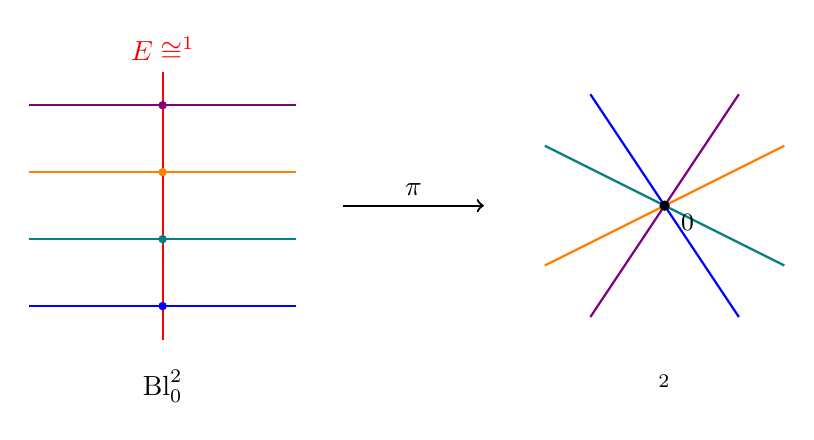
\begin{tikzpicture}[scale=0.85]
% left: blown-up
\begin{scope}[xshift=-4.5cm]
\draw[thick, red] (0,-2) -- (0,2) node[above] {$E\cong\PP^1$};
\foreach \t/\c in {-1.5/blue, -0.5/teal, 0.5/orange, 1.5/violet}{
  \draw[thick, \c] (-2,\t) -- (2,\t);
  \fill[\c] (0,\t) circle (1.8pt);
}
\node at (0,-2.7) {$\mathrm{Bl}_0\C^2$};
\end{scope}
% arrow
\draw[->, thick] (-1.8,0) -- (0.3,0) node[midway, above] {$\pi$};
% right: plane with lines
\begin{scope}[xshift=3cm]
\foreach \t/\c in {-1.5/blue, -0.5/teal, 0.5/orange, 1.5/violet}{
  \draw[thick, \c] ({-2/sqrt(1+\t*\t)},{-2*\t/sqrt(1+\t*\t)}) -- ({2/sqrt(1+\t*\t)},{2*\t/sqrt(1+\t*\t)});
}
\fill (0,0) circle (2.2pt);
\node at (0,-2.7) {$\C^2$};
\node[right] at (0.1,-0.25) {\small $0$};
\end{scope}
\end{tikzpicture}
\caption{$\C^2$ の原点の blow-up の模式図。原点を通る直線（右、色分け）は blow-up 後（左）には互いに交わらず、例外曲線 $E\cong\PP^1$ の異なる点（=直線の傾き $t$）を通る。}
\label{fig:ch15-blowup}
\end{figure}

\begin{myprop}{例外曲線の自己交点数}{ch15-Esquare}
$\mathrm{Bl}_0\C^2$ において $E\cdot E = -1$。すなわち $E$ の法束は $\OO_{\PP^1}(-1)$。
\end{myprop}

\begin{proof}
$\mathrm{Bl}_0\C^2$ は $\OO_{\PP^1}(-1)$ の全空間で、$E$ はその零切断である。全空間の中の零切断の法束はベクトル束自身なので $N_E = \OO(-1)$、$E\cdot E = \deg N_E = -1$。
あるいは関数 $x$ の引き戻しの因子 $(\pi^*x) = E + \tilde L$（$\tilde L$ は直線 $x=0$ の固有変換）が主因子であることから $E\cdot(E+\tilde L) = 0$、$E\cdot\tilde L = 1$ より $E^2 = -1$。
\end{proof}

\paragraph{標準束の変化.}
チャート $(x,t)$、$y = tx$ で
\[
\pi^*(dx\wedge dy) = dx\wedge(t\,dx + x\,dt) = x\,dx\wedge dt .
\]
$\pi^*\Omega$ は $E = \{x=0\}$ に沿って1位で消える。すなわち $K_{\mathrm{Bl}_0\C^2} = \pi^*K_{\C^2} + E$。一般次元では $y_i = t_ix$ として $\pi^*(dx\wedge dy_2\wedge\cdots\wedge dy_n) = x^{n-1}dx\wedge dt_2\wedge\cdots\wedge dt_n$ より
\begin{equation}\label{eq:ch15-discrep}
K_{\mathrm{Bl}_pM} = \pi^*K_M + (n-1)E .
\end{equation}
より一般に、余次元 $c$ の非特異部分多様体 $Z\subset M$ に沿った blow-up では $K = \pi^*K_M + (c-1)E$ で、$E = \PP(N_{Z/M})$ は $Z$ 上の $\PP^{c-1}$ 束である。

\begin{physbox}[非特異点の blow-up は CY 条件を壊す]
式 \eqref{eq:ch15-discrep} より、\emph{非特異}な CY の点を blow-up すると $K$ が非自明（$= (n-1)E$）になり、もはや CY ではない。
弦理論で許されるのは $K$ を変えない操作、すなわち次の小節で述べる crepant な解消である。
\end{physbox}

\subsection{Blow-down}

blow-up の逆操作、すなわち部分多様体を一点（あるいはより低次元の多様体）に潰す双有理射を \textbf{blow-down}（収縮、contraction）という。

\begin{mythm}{Castelnuovo の収縮判定法}{ch15-castelnuovo}
非特異射影曲面 $S$ 上の既約曲線 $E$ が $E\cong\PP^1$ かつ $E\cdot E = -1$ を満たすならば、非特異曲面 $S'$ と点 $p\in S'$ が存在して $S\cong\mathrm{Bl}_pS'$、$E$ はその例外曲線となる。
\end{mythm}

すなわち $(-1)$ 曲線は非特異点に潰せる。一方 $E\cong\PP^1$、$E\cdot E = -2$ の曲線は（Grauert の判定法：負定値な交点行列を持つ曲線は解析的に潰せる）潰すことはできるが、潰した結果は\emph{特異点}（$A_1$ 型）になる。これが次の小節の $\C^2/\Z_2$ の解消の逆である。
一般に、交点行列 $(E_i\cdot E_j)$ が負定値な曲線の配置は正規曲面特異点に潰れる（Grauert）。

3次元では状況が豊かになる。$\PP^1\cong C\subset X$ の法束が $N_C = \OO(-1)\oplus\OO(-1)$ のとき、$C$ を一点に潰すと conifold 特異点が得られる（次の小節）。
このように例外集合が余次元2以上の収縮を\textbf{小収縮}（small contraction）といい、潰した後に「別の方向」に解消し直す操作を\textbf{flop}という。
flop で移り合う2つの CY は双有理同値で Hodge 数も等しいが、一般に異なる（交点数が異なる）多様体である。

\subsection{特異点解消}

\begin{mydef}{特異点解消・crepant 解消}{ch15-resolution}
多様体 $X$ の\textbf{特異点解消}とは、非特異多様体 $\tilde X$ と固有な双有理射 $\pi:\tilde X\to X$ で、$\tilde X\setminus\pi^{-1}(\Sing X)\to X\setminus\Sing X$ が同型であるものをいう。
$X$ が Gorenstein で $K_{\tilde X} = \pi^*K_X$（すべての食い違い係数が $0$）のとき \textbf{crepant 解消}という。
\end{mydef}

広中の定理により、標数 $0$ の多様体は（非特異な中心に沿った blow-up の繰り返しで）常に特異点解消を持つ。しかし crepant 解消は常に存在するとは限らない。
\emph{$X$ が CY なら、crepant 解消 $\tilde X$ もまた $K_{\tilde X}\cong\pi^*\OO_X = \OO_{\tilde X}$ を満たす CY である}。これが CY 条件を保つ解消である。

\begin{myex}{$\C^2/\Z_2$ の解消と $T^*\PP^1$}{ch15-A1res}
$\C^2/\Z_2$（$(z_1,z_2)\mapsto(-z_1,-z_2)$）は $\{uv = w^2\}$、$u = z_1^2$、$v = z_2^2$、$w = z_1z_2$ である。
$\mathrm{Bl}_0\C^2 = \OO_{\PP^1}(-1)$ に $\Z_2$ は $E$ 上自明、ファイバー方向に $-1$ で作用するので（$E$ は固定点集合で余次元 $1$、鏡映的なので商は非特異）、
\[
\widetilde{\C^2/\Z_2} = \mathrm{Bl}_0\C^2/\Z_2 = \text{Tot}\big(\OO_{\PP^1}(-1)^{\otimes2}\big) = \text{Tot}\,\OO_{\PP^1}(-2)\cong T^*\PP^1 .
\]
例外曲線 $C\cong\PP^1$ の自己交点数は $-2$ である。座標で書くと、$\PP^1$ の座標 $\zeta = z_2/z_1$（$\Z_2$ 不変）とファイバー座標 $\xi = z_1^2$ がチャートの座標で、$u = \xi$、$w = \xi\zeta$、$v = \xi\zeta^2$。
\textbf{crepant 性}：$\Omega = dz_1\wedge dz_2$ は $\Z_2$ 不変で $\C^2/\Z_2$ に降りる。$z_2 = \zeta z_1$、$\xi = z_1^2$ より
\[
dz_1\wedge dz_2 = dz_1\wedge(\zeta\,dz_1 + z_1d\zeta) = z_1\,dz_1\wedge d\zeta = \tfrac12\,d\xi\wedge d\zeta .
\]
これは $C = \{\xi = 0\}$ 上でも零にならない。したがって $K_{\widetilde{\C^2/\Z_2}} = \pi^*K$ で、解消は crepant である。
\end{myex}

\begin{myex}{Eguchi--Hanson 計量}{ch15-EH}
$T^*\PP^1$ 上には漸近的に平坦な $\C^2/\Z_2$ に近づく Ricci 平坦 K\"ahler 計量（Eguchi--Hanson 計量）が存在する。$U(2)$ 対称性を仮定して K\"ahler ポテンシャルを $K = F(s)$、$s = |z_1|^2+|z_2|^2$ とおくと、
$g_{i\bar j} = F'\delta_{ij} + F''\bar z_iz_j$ の固有値は $F'$（$z$ に直交する方向）と $F'+sF''$（$z$ 方向）なので
\[
\det g = F'\,(F'+sF'') = \frac{\phi\,\phi'}{s},\qquad \phi := sF'(s).
\]
Ricci 平坦条件 $\rho = -i\partial\bar\partial\log\det g = 0$ は $\det g = 1$ とすれば満たされ、$(\phi^2)' = 2s$、すなわち $\phi = \sqrt{s^2+a^4}$（$a>0$ は積分定数）。積分すると
\[
K = \sqrt{s^2+a^4} + a^2\log\frac{s}{a^2+\sqrt{s^2+a^4}}
\]
を得る（微分して $F' = \sqrt{s^2+a^4}/s$ を確かめよ）。$a = 0$ で平坦計量 $K = s$ に戻る。
$s\to0$ で $\phi\to a^2\neq0$ となり、原点に半径 $\sim a$ の2次元球面 $C$（例外曲線）が現れる。この球面上で計量が滑らかに閉じるのは $\Z_2$ で割ったときに限る。
こうして $a$ は例外曲線の大きさ $\int_C\omega\propto a^2$、すなわち K\"ahler モジュライであり、$a\to0$ が blow-down（特異点への退化）である。
同様に $\C^n$ で $\phi^{n-1}\phi' = s^{n-1}$ を解けば $\phi^n = s^n + a^{2n}$ となり、$\C^n/\Z_n$ の crepant 解消 $\text{Tot}\,K_{\PP^{n-1}}$ 上の Ricci 平坦計量（Calabi 計量）が得られる。
\end{myex}

\begin{myex}{$A_{k-1}$ 特異点の解消}{ch15-Akres}
$x^2+y^2 = z^k$（$\C^2/\Z_k$）の極小解消は、$k-1$ 本の $(-2)$ 曲線 $C_1,\dots,C_{k-1}$ が鎖状に並んだもので、交点行列は
\[
(C_i\cdot C_j) = -\begin{pmatrix}2&-1&&\\-1&2&\ddots&\\&\ddots&\ddots&-1\\&&-1&2\end{pmatrix} = -(\text{$A_{k-1}$ の Cartan 行列})
\]
となる。一般の ADE 特異点でも例外曲線の配置の双対グラフが対応する Dynkin 図形になり、交点行列は Cartan 行列の $-1$ 倍である。
これは2次元の ADE 特異点の解消がすべて crepant であること（Du Val）の反映でもある。
\end{myex}

\begin{myex}{$\C^3/\Z_3$ の解消}{ch15-C3Z3}
$\frac13(1,1,1)$ 型、すなわち $z\mapsto\zeta z$（$\zeta = e^{2\pi i/3}$）。$\det = \zeta^3 = 1$ なので $\SL(3)$ に含まれ Gorenstein。
$\mathrm{Bl}_0\C^3/\Z_3 = \text{Tot}\,\OO_{\PP^2}(-3) = \text{Tot}\,K_{\PP^2}$ が解消で、例外因子は $E\cong\PP^2$。
チャート $\zeta_1 = z_2/z_1$、$\zeta_2 = z_3/z_1$、$\xi = z_1^3$ で
\[
dz_1\wedge dz_2\wedge dz_3 = z_1^2\,dz_1\wedge d\zeta_1\wedge d\zeta_2 = \tfrac13\,d\xi\wedge d\zeta_1\wedge d\zeta_2 ,
\]
したがって crepant である。$\C^3/\Z_3$ は $T^6/\Z_3$ オービフォールド（27個の固定点を持つ）の局所モデルであり、各固定点をこのように解消すると $h^{1,1}$ が $27$ 増える。
\end{myex}

\paragraph{conifold の2通りの滑らかにする方法.}
conifold $\mathcal C = \{xy = uv\}$ には crepant な\textbf{小解消}が2通りある：
\[
\hat{\mathcal C} = \Big\{\big((x,y,u,v),[\lambda_1:\lambda_2]\big)\in\mathcal C\times\PP^1\ \Big|\ \begin{pmatrix}x&u\\v&y\end{pmatrix}\begin{pmatrix}\lambda_1\\\lambda_2\end{pmatrix} = 0\Big\}.
\]
$\det = 0$ なので非零解 $(\lambda_1,\lambda_2)$ が存在し、原点以外では一意、原点では $\PP^1$ 全体が解となる。
チャート $\lambda_1 = 1$、$\lambda_2 = \lambda$ では $x = -u\lambda$、$v = -y\lambda$ なので座標 $(u,y,\lambda)$ で $\C^3$ と同型、すなわち $\hat{\mathcal C}$ は非特異である。
ファイバー座標 $(u,y)$ と別チャートの $(x,v)$ が $\lambda$ 倍で結ばれることから $\hat{\mathcal C} = \text{Tot}\big(\OO_{\PP^1}(-1)\oplus\OO_{\PP^1}(-1)\big)$。
例外集合は曲線 $\PP^1$（余次元2）で例外因子がないので食い違いは生じず、crepant である。
行列の転置を用いた $(\lambda_1,\lambda_2)\begin{pmatrix}x&u\\v&y\end{pmatrix} = 0$ がもう一方の小解消で、両者は flop で移り合う。
（原点を普通に blow-up すると例外因子は $\PP^1\times\PP^1$（2次曲面）で食い違い係数は $1$、crepant ではない。それを2つの $\PP^1$ 方向のどちらかに潰したものが2つの小解消である。）

一方、方程式を変形した
\[
\mathcal C_\varepsilon = \Big\{\sum_{i=1}^4z_i^2 = \varepsilon\Big\},\qquad \varepsilon>0
\]
は非特異で、命題\ref{prop:ch15-conifoldbase}の記号で $|a|^2-|b|^2 = \varepsilon$、$a\cdot b = 0$ となるから $\mathcal C_\varepsilon\cong T^*S^3$（$a/|a|\in S^3$、$b\in T_{a}S^3$）。
$b = 0$ の部分が\textbf{消滅サイクル} $S^3$（半径 $\sqrt\varepsilon$）である。こちらは複素構造の変形であって K\"ahler 類は変えない。
図\ref{fig:ch15-conifold}のとおり、小解消は $S^2$ を、変形は $S^3$ を有限の大きさにする。
コンパクトな CY の中の conifold 点で「変形側」から「解消側」に移る操作が \textbf{conifold transition} であり、その詳細と物理的意味（質量ゼロのブラックホール）は第17章で扱う。

\subsection{解消後の幾何学的構造}

crepant 解消によって位相は変化し、Hodge 数も変わる。基本的な規則は次のとおりである。
\begin{itemize}
\item \textbf{$h^{1,1}$ の増加}：既約な例外因子が1つ現れるごとに、$H^{1,1}$ に新しい類（その例外因子のPoincar\'e双対）が加わる。新しい類の K\"ahler パラメータは例外曲線の大きさを測る（Eguchi--Hanson の $a^2$）。
\item \textbf{K\"ahler 錐の壁}：例外曲線の体積 $\int_C\omega\to0$ の極限は K\"ahler 錐の境界であり、そこで特異 CY に退化する。flop は K\"ahler 錐の壁を越えて隣の錐（別の CY の K\"ahler 錐）に移ることに対応する。
\item \textbf{Euler 数}：点を $\PP^1$ に置き換えると Euler 数は $\chi(\PP^1) - 1 = +1$ 変化する。$N$ 個の conifold 点を持つ $X_0$ について、小解消 $\hat X$ と変形 $X_\varepsilon$ では
\[
\chi(\hat X) = \chi(X_0) + N,\qquad \chi(X_\varepsilon) = \chi(X_0) - N\quad(\chi(S^3) = 0\text{ の点を除くので})
\]
となり、$\chi(\hat X) - \chi(X_\varepsilon) = 2N$。
\end{itemize}

\begin{myex}{$\PP(1,1,2,2,2)[8]$ の解消}{ch15-P11222res}
例\ref{ex:ch15-P11222}の $X_8$ は種数3の曲線 $C$ に沿った $A_1$ 特異点を持つ。$C$ に沿って blow-up すると、例外因子 $E$ は $C$ 上の $\PP^1$ 束（線織面）で、局所的には $C\times T^*\PP^1$ の形をしている。
例\ref{ex:ch15-A1res}の計算が $C$ の各点で成り立つので解消は crepant であり、$\tilde X$ は非特異 CY 3-fold になる。
$H^{1,1}(\tilde X)$ は周囲空間由来の $H$ と例外因子 $E$ で張られて $h^{1,1} = 2$。Euler 数は $\chi(\tilde X) = \chi(X_8) - \chi(C) + \chi(E) = \chi(X_8) + \chi(C)$（$\chi(E) = 2\chi(C)$）で変化し、最終的に $(h^{1,1},h^{2,1}) = (2,86)$ となる。
2つの K\"ahler パラメータは「全体の大きさ」と「$\PP^1$ ファイバーの大きさ」に対応し、後者を零にする極限が特異な $X_8$ である。
\end{myex}

\begin{note}
crepant 解消の存在：$n=2$ の Gorenstein 特異点（= ADE）は常に一意的な crepant 解消（極小解消）を持つ。
$n=3$ では $G\subset\SL(3,\C)$ の商特異点 $\C^3/G$ は常に crepant 解消を持つ（Roan、伊藤、Bridgeland--King--Reid ら。後者は $G$-Hilbert スキームを用いる）が、一意とは限らない（flop で移り合う）。
$n\ge4$ では存在しないこともある：例えば $\C^4/\Z_2$（$-1$ 倍）は端末特異点で crepant 解消を持たない。
解消後の $h^{1,1}$ の増分は、$\C^3/G$ の場合「年齢 $1$ の共役類の数」で与えられる（伊藤--Reid の McKay 対応）。
\end{note}

\exprob{prob:ch15-7-1}
$\C^2/\Z_3$（$(z_1,z_2)\mapsto(\zeta z_1,\zeta^{-1}z_2)$、$\zeta = e^{2\pi i/3}$）が $\{uv = w^3\}$ と同型であることを示せ。
さらに $uv = w^3$ を原点で1回 blow-up すると、例外曲線として1点で交わる2本の $\PP^1$ が現れ、blow-up 後の曲面は非特異であることをチャート計算で確かめよ。
（ヒント：チャート $u = u$, $v = uv'$, $w = uw'$ では $v' = uw'^3$ となる。）

\exprob{prob:ch15-7-2}
conifold $\mathcal C = \{xy = uv\}$ の小解消 $\hat{\mathcal C}$ において、正則3形式
$\Omega = \dfrac{dx\wedge du\wedge dv}{x}$（$\mathcal C$ 上で $y = uv/x$ として）を、チャート座標 $(u,y,\lambda)$（$x = -u\lambda$, $v = -y\lambda$）で表し、
例外曲線の上でも至る所正則かつ非零であることを確かめよ。

% ============================================================
\section{弦理論におけるCalabi--Yau}
% ============================================================

本節では、ここまでに構成した Calabi--Yau 多様体がなぜ弦理論の余剰次元として選ばれるのかを説明し、
Hodge 数・交点数といった幾何学的データが4次元の物理（超対称性の数、粒子の世代数、質量ゼロのスカラー場の数、結合定数）をどのように決めるかを見る。
物理的な導出は概略にとどめ、代数幾何との対応を明確にすることを主眼とする。

\subsection{超弦理論における余剰次元}

超弦理論は時空の次元 $D$ が $10$ のときにのみ無矛盾に量子化できる。世界面（第13章で見た Riemann 面）上の共形場理論の言葉で言えば、
Weyl アノマリーの相殺条件、すなわち物質の中心電荷 $c$ がゴースト系の寄与と打ち消し合う条件が
\[
\text{ボソン弦：}\ D = 26,\qquad\text{超弦：}\ \tfrac32D = 15\ \Longrightarrow\ D = 10
\]
を与える（時空座標 $X^\mu$ 一つあたりボソンが $1$、Majorana フェルミオンが $\frac12$ の中心電荷を持つ）。
10次元の超弦理論には5種類（タイプ IIA、IIB、I、ヘテロティック $E_8\times E_8$、$SO(32)$）あり、いずれも10次元の超重力理論を低エネルギー有効理論として持つ。

観測される時空は4次元なので、残りの6次元は観測にかからないほど小さくコンパクトでなければならない。そこで時空を
\[
M_{10} = M_4\times X_6
\]
と仮定する（図\ref{fig:ch15-10=4+6}）。ここで $M_4$ は4次元 Minkowski 時空、$X_6$ は実6次元のコンパクト多様体（内部空間）である。
これが「$10 = 4+6$」の分解であり、内部空間の幾何が4次元の物理を決める。

\begin{figure}[H]
\centering
\begin{tikzpicture}[scale=0.75]
\draw[thick] (-4,-1) -- (3,-1) -- (4.5,1.2) -- (-2.5,1.2) -- cycle;
\node at (-3.2,1.6) {$M_4$（4次元 Minkowski 時空、大きい）};
\foreach \x/\y in {-2.6/-0.5, -0.9/-0.5, 0.8/-0.5, 2.5/-0.5, -1.7/0.55, 0/0.55, 1.7/0.55, 3.3/0.55}{
  \begin{scope}[shift={(\x,\y)}]
  \draw[fill=orange!30, draw=orange!70!black] (0,0) .. controls (0.25,0.35) and (0.5,0.05) .. (0.35,-0.15)
     .. controls (0.2,-0.35) and (-0.2,-0.3) .. (-0.3,-0.1) .. controls (-0.4,0.1) and (-0.2,0.3) .. (0,0);
  \end{scope}
}
\draw[->, thick] (5.0,0.0) -- (6.2,0.0);
\begin{scope}[shift={(7.4,0)}, scale=1.6]
  \draw[fill=orange!30, draw=orange!70!black, thick] (0,0) .. controls (0.25,0.35) and (0.5,0.05) .. (0.35,-0.15)
     .. controls (0.2,-0.35) and (-0.2,-0.3) .. (-0.3,-0.1) .. controls (-0.4,0.1) and (-0.2,0.3) .. (0,0);
  \node[below] at (0,-0.4) {$X_6$};
  \node[below] at (0,-0.75) {\small CY 3-fold};
\end{scope}
\end{tikzpicture}
\caption{$10 = 4+6$ の模式図。4次元時空の各点に、小さなコンパクト6次元多様体 $X_6$（Calabi--Yau 3-fold）が付随している。}
\label{fig:ch15-10=4+6}
\end{figure}

\subsection{コンパクト化}

内部空間がコンパクトであるとき、10次元の場を内部空間の固有関数で展開すると4次元の場の無限個の塔が得られる。これを Kaluza--Klein（KK）コンパクト化という。

\begin{myex}{円周上のコンパクト化}{ch15-KK}
5次元のスカラー場 $\Phi(x,y)$（$x\in M_4$、$y\in S^1$、周期 $2\pi R$）が $\Box_5\Phi = 0$ を満たすとする。Fourier 展開
\[
\Phi(x,y) = \sum_{k\in\Z}\phi_k(x)\,e^{iky/R}
\]
を代入すると $\big(\Box_4 - k^2/R^2\big)\phi_k = 0$。すなわち4次元では質量 $m_k = |k|/R$ の粒子の塔が現れる。
$R$ が小さければ $k\neq0$ のモードは非常に重く、低エネルギーでは\emph{内部空間の Laplace 作用素の零モード}（$k=0$）だけが残る。
さらに5次元計量 $g_{55}$ 成分は4次元のスカラー場 $R(x)$（半径の揺らぎ）を与える。その値は古典的にはポテンシャルを持たず任意で、
これが\textbf{モジュライ場}の最も簡単な例である。
\end{myex}

一般に、内部空間 $X$ 上の $p$ 形式場 $C_p$ の質量ゼロのモードは、$X$ 上の調和 $p$ 形式（Hodge 理論により de Rham コホモロジー $H^p(X)$ と同型）で数えられる：
\[
C_p(x,y) = \sum_{k}\sum_{a=1}^{b_k(X)}c^{(a)}_{p-k}(x)\wedge\eta^{(k)}_a(y),\qquad \eta^{(k)}_a\in\mathcal H^k(X).
\]
すなわち\emph{4次元の質量ゼロの場の数は内部空間の Betti 数（複素多様体なら Hodge 数）で決まる}。これが代数幾何的な位相不変量が物理に直結する基本的な機構である。

\subsection{内部空間の幾何学}

内部空間 $X_6$ に課される条件を順に見る。
\begin{enumerate}
\item \textbf{コンパクト性}：4次元の重力定数を有限にするため（$1/G_4\propto\mathrm{Vol}(X)/G_{10}$）。
\item \textbf{運動方程式}：最低次（フラックスなし、ディラトン一定）の10次元超重力の真空方程式は $R_{MN} = 0$。$M_4$ が平坦なら $X$ は \textbf{Ricci 平坦}でなければならない。
\item \textbf{4次元の超対称性}：低エネルギー物理（階層性問題、ゲージ結合の統一など）の観点から、4次元で $\mathcal N=1$ 超対称性が残ることが望ましい。
これが以下で見るように $X$ に\textbf{共変定数スピノル}の存在を要求し、ホロノミーを $SU(3)$ に制限する。
\end{enumerate}

\paragraph{超対称性の条件.}
10次元超重力の超対称性変換のうち、グラビティーノ $\psi_M$ の変換は（フラックス $H = 0$、ディラトン一定のとき）
\[
\delta_\varepsilon\psi_M = \nabla_M\varepsilon
\]
である。ボソン的背景が超対称性を保つとは、フェルミオンの変換がすべて零となる $\varepsilon\neq0$ が存在すること（Killing スピノル方程式）である。
10次元の Majorana--Weyl スピノル $\varepsilon$ を $M_4\times X_6$ に合わせて $\varepsilon = \zeta\otimes\eta + (\text{c.c.})$（$\zeta$ は4次元の定数 Weyl スピノル、$\eta$ は $X$ 上のスピノル）と分解すると、条件は
\[
\nabla_m\eta = 0\qquad(m = 1,\dots,6)
\]
すなわち $X$ が\textbf{共変定数（平行）スピノル}を持つことになる。

\begin{mythm}{共変定数スピノルと $SU(3)$ ホロノミー}{ch15-spinor}
向き付けられた6次元 Riemann スピン多様体 $(X,g)$ が非零の共変定数 Weyl スピノル $\eta$ を持つための必要十分条件は $\mathrm{Hol}(g)\subset SU(3)$ である。
このとき $(X,g)$ は Ricci 平坦 K\"ahler 多様体であり、$K_X$ は平坦（$X$ が単連結なら自明）である。
\end{mythm}

\begin{proof}[論証の概略]
\textbf{ホロノミー}：平行なスピノルはホロノミー群（のスピン群への持ち上げ）で不変である。$\mathrm{Spin}(6)\cong SU(4)$ で、正のカイラリティーの Weyl スピノルは $SU(4)$ の基本表現 $\mathbf 4$ である。
零でないベクトル $\eta\in\C^4$ の $SU(4)$ における安定化群は $SU(3)$（$\mathbf 4 = \mathbf 3\oplus\mathbf 1$ と分解したときの $\mathbf 1$ 方向を固定する部分群）なので、$\mathrm{Hol}\subset SU(3)$。
逆に $\mathrm{Hol}\subset SU(3)$ なら $\mathbf 4\to\mathbf 3\oplus\mathbf1$ の不変成分 $\mathbf 1$ を平行移動で広げて平行スピノルが得られる。

\textbf{幾何構造}：$\eta^\dagger\eta = 1$ と規格化し、Clifford 代数のガンマ行列 $\gamma_m$ を用いて
\[
J_m{}^n = i\,\eta^\dagger\gamma_m{}^n\eta,\qquad \Omega_{mnp} = \eta^{T}C\gamma_{mnp}\eta\quad(C\text{ は荷電共役行列})
\]
と定める。Fierz 恒等式から $J_m{}^nJ_n{}^p = -\delta_m{}^p$ で $J$ は概複素構造、$\eta$ が平行なので $J$ も $\Omega$ も平行。
$\nabla J = 0$ より $(X,g,J)$ は K\"ahler（定理\ref{thm:ch15-kahlercond}(5)）、$\Omega$ は平行な $(3,0)$ 形式で正則体積形式を与える。

\textbf{Ricci 平坦性}（積分可能条件）：$[\nabla_m,\nabla_n]\eta = \frac14R_{mnpq}\gamma^{pq}\eta = 0$。これに $\gamma^n$ を掛け、
$\gamma^n\gamma^{pq} = \gamma^{npq}+g^{np}\gamma^q - g^{nq}\gamma^p$ と第一 Bianchi 恒等式 $R_{m[npq]} = 0$（$\gamma^{npq}$ の項が消える）を使うと
\[
R_{mq}\gamma^q\eta = 0 .
\]
$\gamma^q\eta$（$q=1,\dots,6$）は実ベクトル $v$ に対して $v_q\gamma^q\eta = 0\Rightarrow v = 0$ を満たす（$v_q\gamma^q$ の2乗は $|v|^2$）ので、$R_{mq} = 0$。
\end{proof}

したがって、超対称性を保つ（フラックスのない）コンパクト化の内部空間は\emph{ホロノミーが $SU(3)$ に含まれるコンパクト Ricci 平坦 K\"ahler 3-fold}、すなわち（広義の）Calabi--Yau 3-fold である。
Yau の定理（定理\ref{thm:ch15-yau}）のおかげで、このような計量の存在は $c_1(X) = 0$ という\emph{位相的・代数的}条件に帰着し、15.5〜15.7節の代数幾何的構成がそのまま使える。
これが Candelas--Horowitz--Strominger--Witten（1985）の発見の核心である。

\subsection{Calabi--Yauコンパクト化}

\paragraph{超対称性の数.}
平行スピノルの数はホロノミー群で決まる。$\mathbf 4$ の中の不変成分の数を数えると
\begin{center}
\small\renewcommand{\arraystretch}{1.3}
\begin{tabular}{c|c|c|c|c}
$X_6$ & $\mathrm{Hol}$ & 平行スピノル & ヘテロティック（16 個）& タイプ II（32 個）\\ \hline
$T^6$ & $\{1\}$ & $4$ & 4次元 $\mathcal N=4$ & 4次元 $\mathcal N=8$\\
$K3\times T^2$ & $SU(2)$ & $2$ & $\mathcal N=2$ & $\mathcal N=4$\\
strict CY 3-fold & $SU(3)$ & $1$ & $\mathcal N=1$ & $\mathcal N=2$\\
\end{tabular}
\end{center}
（10次元のヘテロティック弦は 16 個、タイプ II は 32 個の超電荷を持ち、それぞれ $1/4$ が保たれる：4次元 $\mathcal N=1$ は4個の超電荷。）
4次元 $\mathcal N=1$ はカイラルなフェルミオンを許す唯一の拡張であり、標準模型の構造と整合する。
これが\emph{ヘテロティック弦の strict CY 3-fold 上のコンパクト化}が現実的な模型の出発点とされた理由である。
ここで (CY2) の条件 $h^{1,0}=h^{2,0}=0$ が、ちょうど「超対称性が多すぎない」ことに対応している点に注意する。

\paragraph{ゲージ束と標準埋め込み.}
ヘテロティック弦ではさらに、ゲージ場 $A$ が $X$ 上の正則ベクトル束 $V$ の Hermite--Yang--Mills 接続であること
（$F^{2,0} = F^{0,2} = 0$、$\omega^{2}\wedge F = 0$；第14章）と、アノマリー相殺条件
\[
dH = \frac{\alpha'}{4}\big(\Tr R\wedge R - \Tr F\wedge F\big)\ \Longrightarrow\ c_2(V) = c_2(T_X)\quad(H=0\text{ のとき})
\]
が要求される。最も簡単な解は $V = T_X$、すなわちゲージ接続をスピン接続（$SU(3)$ に値を持つ）に等しくとる\textbf{標準埋め込み}である。
$E_8\supset SU(3)\times E_6$ の $SU(3)$ に埋め込むと、4次元に残るゲージ群は $SU(3)$ の中心化群 $E_6$（大統一群）になり、随伴表現は
\[
\mathbf{248} = (\mathbf{78},\mathbf1)\oplus(\mathbf1,\mathbf8)\oplus(\mathbf{27},\mathbf3)\oplus(\overline{\mathbf{27}},\overline{\mathbf3})
\]
と分解する。$(\mathbf{27},\mathbf3)$ 成分を持つ10次元ゲージーノの零モードが4次元の物質（クォーク・レプトンの世代）を与える。

\subsection{幾何学的自由度と物理的自由度}

\paragraph{世代数.}
$\mathbf{27}$ の零モードは $T_X$ に値を持つ $\bar\partial$ 作用素の零モード、すなわち $H^1(X,T_X)$ で、$\overline{\mathbf{27}}$ の零モードは $H^1(X,T^*_X)$ で数えられる。
命題\ref{prop:ch15-cy-prop}(3)より
\[
n_{\mathbf{27}} = \dim H^1(X,T_X) = h^{2,1},\qquad n_{\overline{\mathbf{27}}} = \dim H^1(X,T^*_X) = h^{1,1}.
\]
$\mathbf{27}$ と $\overline{\mathbf{27}}$ は対になって質量を得うるので、低エネルギーに残る\textbf{正味の世代数}は
\[
N_{\rm gen} = \big|n_{\mathbf{27}} - n_{\overline{\mathbf{27}}}\big| = |h^{2,1}-h^{1,1}| = \frac{|\chi(X)|}{2}
\]
である。物理の世代数が Euler 数という位相不変量で決まる、というのは驚くべき結論である。
\begin{itemize}
\item quintic：$|\chi|/2 = 100$ 世代。現実（3世代）からは程遠い。
\item 3世代を得るには $|\chi| = 6$ の CY が必要である。歴史的に最初の例は Tian--Yau 多様体：$\PP^3\times\PP^3$ の完全交差
$\left[\begin{smallmatrix}\PP^3 & 3 & 0 & 1\\ \PP^3 & 0 & 3 & 1\end{smallmatrix}\right]$（$\chi = -18$）を、自由に作用する $\Z_3$ で割った商で、$\chi = -18/3 = -6$。
（有限群 $G$ が自由に作用すれば $\chi(X/G) = \chi(X)/|G|$。また商でも $\Omega$ が $G$ 不変なら CY のまま。）
\end{itemize}

\paragraph{モジュライ場.}
Ricci 平坦計量の変形（質量ゼロのスカラー場）を数える。$g + \delta g$ が再び Ricci 平坦であるための線形化条件（Lichnerowicz 方程式）を解くと、変形は二種類に分かれる。
\begin{itemize}
\item \textbf{K\"ahler 変形} $\delta g_{i\bar j}$：$i\,\delta g_{i\bar j}dz^i\wedge d\bar z^j$ は調和 $(1,1)$ 形式で、$h^{1,1}$ 個。K\"ahler 類 $[\omega]$ の変化に対応する（Yau の定理によって各 K\"ahler 類に一意の Ricci 平坦計量があることと整合）。
\item \textbf{複素構造変形} $\delta g_{\bar i\bar j}$：$\Omega$ を用いて $\Omega_{ijk}\,g^{k\bar l}\delta g_{\bar l\bar m}\,dz^i\wedge dz^j\wedge d\bar z^m$ を作ると調和 $(2,1)$ 形式となり、$h^{2,1}$ 個（複素パラメータ）。
これは $H^1(X,T_X)\cong H^{2,1}$（式\eqref{eq:ch15-TOmega}）の Kodaira--Spencer 類である。
\end{itemize}
弦理論では計量の他に $B$ 場（2形式場）があり、その調和成分 $B = \sum b^a\omega_a$ と K\"ahler 形式 $J = \sum t^a\omega_a$ を組にして
\[
B + iJ = \sum_{a=1}^{h^{1,1}}(b^a+it^a)\,\omega_a
\]
と\textbf{複素化された K\"ahler モジュライ} $h^{1,1}$ 個を得る。したがって4次元の質量ゼロの中性スカラー場（モジュライ場）として
\[
h^{1,1}\ \text{個の（複素化）K\"ahler モジュライ},\qquad h^{2,1}\ \text{個の複素構造モジュライ}
\]
が現れる（これにディラトン等が加わる）。quintic では $1$ 個と $101$ 個である。
タイプ II 弦ではこれらは4次元 $\mathcal N=2$ 超多重項に組み込まれる：タイプ IIA では $h^{1,1}$ 個のベクトル多重項と $h^{2,1}+1$ 個のハイパー多重項、
タイプ IIB では $h^{2,1}$ 個のベクトル多重項と $h^{1,1}+1$ 個のハイパー多重項。IIA と IIB で $h^{1,1}$ と $h^{2,1}$ の役割が入れ替わることが、ミラー対称性（第17章）の物理的な動機の一つである。
モジュライ空間の局所構造・特殊 K\"ahler 幾何は第16章で詳しく扱う。

\begin{physbox}[幾何と物理の辞書]
\begin{center}
\small\renewcommand{\arraystretch}{1.25}
\begin{tabular}{p{0.4\linewidth}|p{0.5\linewidth}}
幾何（Calabi--Yau 3-fold $X$）& 物理（4次元有効理論）\\ \hline
$\mathrm{Hol} = SU(3)$（平行スピノル1個）& ヘテロティックで $\mathcal N=1$、タイプ II で $\mathcal N=2$ 超対称性\\
$h^{1,1}$（K\"ahler 類 $+$ $B$ 場）& K\"ahler モジュライ場の数、$\overline{\mathbf{27}}$ の数\\
$h^{2,1}$（$H^1(T_X)$）& 複素構造モジュライ場の数、$\mathbf{27}$ の数\\
$|\chi|/2 = |h^{1,1}-h^{2,1}|$ & 正味の世代数\\
三重交点数 $\int_X\omega_a\wedge\omega_b\wedge\omega_c$ & $\overline{\mathbf{27}}^3$ 湯川結合（古典的部分）\\
$\int_X\Omega\wedge\partial_a\partial_b\partial_c\Omega$ & $\mathbf{27}^3$ 湯川結合\\
特異点（conifold、ADE）& 質量ゼロの粒子、ゲージ対称性の増大\\
\end{tabular}
\end{center}
\end{physbox}

\subsection{Calabi--Yau幾何の物理的意味}

\paragraph{湯川結合.}
4次元の超ポテンシャルに現れる $\mathbf{27}^3$ 型の湯川結合は、複素構造モジュライ $z^a$（$a=1,\dots,h^{2,1}$）の関数として
\[
\kappa_{abc}(z) = \int_X\Omega(z)\wedge\frac{\partial^3\Omega(z)}{\partial z^a\partial z^b\partial z^c}
\]
で与えられ、$\Omega$ の周期積分から計算できる（第16章の特殊幾何）。これは複素構造のみに依存する正則な量で、量子補正を受けない。
一方 $\overline{\mathbf{27}}^3$ 型の湯川結合は K\"ahler モジュライ $t^a$ の関数で、古典的には三重交点数
\[
\kappa_{abc}^{\rm cl} = \int_X\omega_a\wedge\omega_b\wedge\omega_c
\]
（quintic では $\int_XH^3 = 5$）で与えられるが、世界面インスタントン（$X$ の中の正則曲線に巻きついた弦）による補正を受ける。
quintic の場合、$q = e^{2\pi it}$ として
\[
\kappa_{ttt} = 5 + \sum_{d\geq1}n_d\,d^3\frac{q^d}{1-q^d},\qquad n_1 = 2875,\ n_2 = 609250,\ \dots
\]
となり、$n_d$ は quintic 上の次数 $d$ の有理曲線の数（$n_1 = 2875$ は quintic 上の直線の数）である。
これを複素構造側の周期計算から求めるのがミラー対称性であり（第17章）、Dwork 族（例\ref{ex:ch15-dwork}）がその主役となる。

\paragraph{特異点の物理.}
CY のモジュライ空間の中で、15.7節の特異点は特別な点として現れる。
\begin{itemize}
\item \textbf{conifold 点}：消滅する $S^3$ に巻きついた D3 ブレーンが質量ゼロのハイパー多重項（荷電ブラックホール）となり、有効理論の特異性を解消する（Strominger）。
変形側と小解消側を結ぶ conifold transition は、異なる Hodge 数を持つ CY を物理的に連続につなぐ（第17章）。
\item \textbf{曲線に沿った ADE 特異点}：消滅する $(-2)$ 曲線に巻きついた D2 ブレーン（タイプ IIA）が質量ゼロの W ボソンとなり、非可換ゲージ対称性 $G_{ADE}$ が現れる。これは F 理論（第17章）での模型構築の基本である。
\item \textbf{オービフォールド}：$T^6/\Z_3$ のような特異な空間上でも弦理論は無矛盾に定義され（ねじれセクター）、その質量ゼロモードは crepant 解消の例外因子の数とちょうど一致する（弦理論的 Euler 数 $=$ 解消後の Euler 数）。
\end{itemize}

\paragraph{まとめ.}
本章で学んだことを振り返ると、
\begin{enumerate}
\item 超対称性 $\Rightarrow$ 平行スピノル $\Rightarrow$ $\mathrm{Hol}\subset SU(3)$ $\Leftrightarrow$ Ricci 平坦 K\"ahler $\Leftrightarrow$（Yau）$c_1 = 0$、という鎖によって、微分方程式の問題が代数幾何の問題に置き換わる。
\item $c_1 = 0$ の多様体は、随伴公式 $K_X = (K_{\PP^N}\otimes\OO(d))|_X$ と $K_{\PP^N} = \OO(-N-1)$ により $d = N+1$（完全交差なら $\sum d_a = N+1$、重み付きなら $d = \sum w_i$）として大量に構成できる。
\item 4次元の物理（世代数、モジュライ場の数、湯川結合）は Hodge 数・Euler 数・交点数・周期といった代数幾何的不変量で書かれる。
\end{enumerate}
次の第16章ではこれらのモジュライ空間の構造を、第17章ではミラー対称性・conifold transition・F 理論を扱う。

\exprob{prob:ch15-8-1}
ヘテロティック弦を次の CY 3-fold 上で標準埋め込みによりコンパクト化したとき、$\mathbf{27}$ と $\overline{\mathbf{27}}$ の数および正味の世代数を求めよ：
(a) quintic $\PP^4[5]$、(b) $\PP^5[3,3]$、(c) $\PP^2\times\PP^2$ の双次数 $(3,3)$ 超曲面、(d) $\PP(1,1,2,2,2)[8]$ の解消。

\exprob{prob:ch15-8-2}
$\mathrm{Spin}(6)\cong SU(4)$ の下で、$\mathrm{Spin}(1,9)$ の Majorana--Weyl スピノル $\mathbf{16}$ が $SL(2,\C)\times SU(4)$ の表現として $(\mathbf2,\mathbf4)\oplus(\bar{\mathbf2},\bar{\mathbf4})$ と分解することを認めて、
$SU(4)\supset SU(3)$ による分解 $\mathbf4 = \mathbf3\oplus\mathbf1$ から、ホロノミー $SU(3)$ の内部空間でヘテロティック弦の16個の超電荷のうち4個が残ること（4次元 $\mathcal N=1$）を説明せよ。
内部空間が $T^6$（ホロノミー自明）や $K3\times T^2$（ホロノミー $SU(2)$）の場合にはどうなるか。

\section*{問題の解答}
\addcontentsline{toc}{section}{問題の解答}

\exsol{prob:ch15-1-1}
$U_0\cap U_1$ 上で $z_1 = Z_1/Z_0 = 1/w_0$、$z_i = Z_i/Z_0 = (Z_i/Z_1)(Z_1/Z_0) = w_i/w_0$（$i\ge2$）である。微分すると
\[
dz_1 = -w_0^{-2}\,dw_0,\qquad dz_i = w_0^{-1}dw_i - w_iw_0^{-2}\,dw_0\quad(i\ge2).
\]
外積 $dz_1\wedge dz_2\wedge\cdots\wedge dz_n$ では $dz_1$ がすでに $dw_0$ に比例するので、$dz_i$（$i\ge 2$）の $dw_0$ 成分はすべて落ちる。したがって
\[
dz_1\wedge dz_2\wedge\cdots\wedge dz_n = (-w_0^{-2}dw_0)\wedge(w_0^{-1}dw_2)\wedge\cdots\wedge(w_0^{-1}dw_n)
= -\,w_0^{-(n+1)}\,dw_0\wedge dw_2\wedge\cdots\wedge dw_n .
\]
すなわち $U_0$ 上の $K_{\PP^n}$ の枠 $e_0 = dz_1\wedge\cdots\wedge dz_n$ と $U_1$ 上の枠 $e_1 = dw_0\wedge dw_2\wedge\cdots\wedge dw_n$ は $e_0 = -w_0^{-(n+1)}e_1$ で結ばれる。

一方 $\OO(k)$ の枠は $Z_0^k = w_0^kZ_1^k$ で結ばれるから、$k = -(n+1)$ とすると $Z_0^{-(n+1)} = w_0^{-(n+1)}Z_1^{-(n+1)}$。
符号 $-1$ を除いて変換係数が一致する。符号を大域的に処理するには次のようにすればよい。
$\Omega_0 = \sum_{i=0}^n(-1)^iZ_i\,dZ_0\wedge\cdots\wedge\widehat{dZ_i}\wedge\cdots\wedge dZ_n$ は Euler ベクトル場 $E = \sum Z_i\partial/\partial Z_i$ による縮約 $\iota_E(dZ_0\wedge\cdots\wedge dZ_n)$ である。
$U_0$ 上の座標 $(Z_0,z_1,\dots,z_n)$（$Z_i = Z_0z_i$）では $dZ_0\wedge\cdots\wedge dZ_n = Z_0^n\,dZ_0\wedge dz_1\wedge\cdots\wedge dz_n$、$E = Z_0\partial/\partial Z_0$ なので
$\Omega_0 = Z_0^{n+1}\,dz_1\wedge\cdots\wedge dz_n$。同様に $U_1$ 上の座標 $(Z_1,w_0,w_2,\dots,w_n)$ では
$dZ_0\wedge dZ_1\wedge\cdots\wedge dZ_n = Z_1^n\,dw_0\wedge dZ_1\wedge dw_2\wedge\cdots\wedge dw_n = -Z_1^n\,dZ_1\wedge dw_0\wedge dw_2\wedge\cdots\wedge dw_n$ より
$\Omega_0 = -Z_1^{n+1}e_1$。そこで各 $U_i$ 上の枠を
\[
\varepsilon_i := \frac{\Omega_0}{Z_i^{n+1}}\qquad(\varepsilon_0 = e_0,\ \varepsilon_1 = -e_1)
\]
と取り直すと（$\Omega_0$ は次数 $n+1$ の斉次式なので $\varepsilon_i$ は $U_i$ 上の well-defined な正則 $n$ 形式で、至る所零でない）、恒等的に
\[
\varepsilon_i = \Big(\frac{Z_j}{Z_i}\Big)^{n+1}\varepsilon_j ,\qquad\text{一方}\qquad Z_i^{-(n+1)} = \Big(\frac{Z_j}{Z_i}\Big)^{n+1}Z_j^{-(n+1)}
\]
が成り立つ。$i=0$, $j=1$ では $\varepsilon_0 = w_0^{-(n+1)}\varepsilon_1$ で、上の直接計算と一致する。
遷移関数がすべてのチャートの組で一致するので、$\varepsilon_i\leftrightarrow Z_i^{-(n+1)}$ によって $K_{\PP^n}\cong\OO(-n-1)$ である。

\exsol{prob:ch15-1-2}
$J^2 = -1$ を用いると
\[
J\big(v - iJv\big) = Jv - iJ^2v = Jv + iv = i\big(v - iJv\big)
\]
なので $J v^{1,0} = i\,v^{1,0}$。また $v\neq0$ なら $v^{1,0}$ の実部は $\frac12v\neq0$ なので $v^{1,0}\neq0$ であり、$v^{1,0}$ は固有値 $i$ の固有ベクトルである。
$v = \partial_x$ のとき $Jv = \partial_y$ だから $v^{1,0} = \frac12(\partial_x - i\partial_y) = \partial_z$。
（同様に $v = \partial_y$ なら $Jv = -\partial_x$ で $v^{1,0} = \frac12(\partial_y + i\partial_x) = i\partial_z$ となり、$v\mapsto v^{1,0}$ は $J$ を $i$ 倍に写す複素線形同型 $TX\cong T^{1,0}X$ を与える。）

\exsol{prob:ch15-2-1}
$f$ が正則なら $\partial_{\bar j}f = 0$、また $\bar f$ は反正則なので $\partial_i\bar f = \overline{\partial_{\bar i}f} = 0$。よって
\[
\partial_i\partial_{\bar j}(f+\bar f) = \partial_i\big(\partial_{\bar j}f\big) + \partial_{\bar j}\big(\partial_i\bar f\big) = 0,
\]
すなわち $\partial_i\partial_{\bar j}(K+f+\bar f) = \partial_i\partial_{\bar j}K = g_{i\bar j}$ で、計量（および $\omega = i\partial\bar\partial K$）は変わらない。

Fubini--Study の場合、$|w|^2 = \sum_{i\neq1}|w_i|^2$ とすると $1+|w|^2 = |Z|^2/|Z_1|^2$、$1+|z|^2 = |Z|^2/|Z_0|^2$ なので、$U_0\cap U_1$ 上で
\[
\log(1+|z|^2) = \log(1+|w|^2) + \log\frac{|Z_1|^2}{|Z_0|^2} = \log(1+|w|^2) + \log|z_1|^2 .
\]
$U_0\cap U_1$ 上では $z_1\neq0$ なので、各点の近傍で $\log z_1$ の分枝 $f$ が取れ、$\log|z_1|^2 = f+\bar f$（$f$ は正則）となる。
前半により、二つのポテンシャルは各点の近傍で同じ $i\partial\bar\partial(\,\cdot\,)$ を与える。$\omega = i\partial\bar\partial K$ は座標によらない 2 形式であり、計量 $g$ は $\omega$ から $g(X,Y) = \omega(X,JY)$ で復元されるので、
$z$ 座標で $\log(1+|z|^2)$ から計算した計量と $w$ 座標で $\log(1+|w|^2)$ から計算した計量は $U_0\cap U_1$ 上で一致する。

\exsol{prob:ch15-2-2}
Christoffel 記号の公式は座標ベクトル場に関して代数的（$\C$ 上多重線形に拡張できる）なので、複素座標 $(z^i,\bar z^i)$ と添字 $\mu,\nu,\ldots\in\{i,\bar i\}$ でそのまま使える。
Hermitian 計量では $g_{ij} = g_{\bar i\bar j} = 0$ で、非零成分は $g_{i\bar j} = g_{\bar ji}$ のみ。その逆行列の非零成分も $g^{k\bar l} = g^{\bar lk}$（$g^{k\bar l}g_{j\bar l} = \delta^k_j$）のみである。したがって上付き添字が $k$ のとき和は $\rho = \bar l$ の項だけが残り、
\[
\Gamma^k_{\mu\nu} = \tfrac12 g^{k\bar l}\big(\partial_\mu g_{\bar l\nu} + \partial_\nu g_{\bar l\mu} - \partial_{\bar l}g_{\mu\nu}\big).
\]
K\"ahler 条件 $\partial_kg_{i\bar j} = \partial_ig_{k\bar j}$ の複素共役は、$\overline{g_{i\bar j}} = g_{j\bar i}$ より $\partial_{\bar k}g_{j\bar i} = \partial_{\bar i}g_{j\bar k}$、すなわち $\partial_{\bar j}g_{i\bar l} = \partial_{\bar l}g_{i\bar j}$ である。下付き添字の型で場合分けする。
\begin{itemize}
\item $(\mu,\nu) = (i,j)$：$g_{ij} = 0$ と K\"ahler 条件 $\partial_jg_{i\bar l} = \partial_ig_{j\bar l}$ より
$\Gamma^k_{ij} = \frac12g^{k\bar l}(\partial_ig_{j\bar l} + \partial_jg_{i\bar l}) = g^{k\bar l}\partial_ig_{j\bar l}$。
\item $(\mu,\nu) = (i,\bar j)$：$g_{\bar l\bar j} = 0$ より $\Gamma^k_{i\bar j} = \frac12g^{k\bar l}(\partial_{\bar j}g_{i\bar l} - \partial_{\bar l}g_{i\bar j}) = 0$（共役な K\"ahler 条件）。$\Gamma$ は下付き添字について対称なので $\Gamma^k_{\bar ji} = 0$ も従う。
\item $(\mu,\nu) = (\bar i,\bar j)$：括弧内の三項はすべて $g_{\bar l\bar j}$、$g_{\bar l\bar i}$、$g_{\bar i\bar j}$ の微分で零。よって $\Gamma^k_{\bar i\bar j} = 0$。
\end{itemize}
上付き添字が $\bar k$ のものは、$g$ が実なので $\Gamma^{\bar k}_{\bar\mu\bar\nu} = \overline{\Gamma^k_{\mu\nu}}$ であり、上の結果の複素共役から $\Gamma^{\bar k}_{\bar i\bar j} = \overline{\Gamma^k_{ij}}$ 以外は零である。
（K\"ahler 条件は $\Gamma^k_{ij}$ が $i,j$ について対称な形 $g^{k\bar l}\partial_ig_{j\bar l}$ に書けることと、混合型の消滅の両方に使われている。）

\exsol{prob:ch15-3-1}
$U_0$ 上の枠 $Z_0^k$ に関して $h = |Z_0^k|^2/|Z|^{2k} = (1+|z|^2)^{-k}$ であり、$U_1$ 上でも枠 $Z_1^k$ について $(1+|w|^2)^{-k}$ なので、これは $\PP^1$ 全体の Hermitian 計量である。
直線束の Chern 曲率は式 \eqref{eq:ch15-trTheta} より $\Theta = \bar\partial\partial\log h = -\partial\bar\partial\log h = k\,\partial\bar\partial\log(1+|z|^2)$。ここで
\[
\partial_{\bar z}\log(1+z\bar z) = \frac{z}{1+|z|^2},\qquad
\partial_z\frac{z}{1+|z|^2} = \frac{(1+|z|^2) - z\bar z}{(1+|z|^2)^2} = \frac{1}{(1+|z|^2)^2}
\]
なので
\[
\frac{i}{2\pi}\Theta = \frac{ik}{2\pi}\,\frac{dz\wedge d\bar z}{(1+|z|^2)^2} = \frac{k}{2\pi}\,\frac{2\,dx\wedge dy}{(1+r^2)^2}\qquad(r = |z|)
\]
（$i\,dz\wedge d\bar z = 2\,dx\wedge dy$）。$\PP^1\setminus U_0$ は 1 点で測度零だから、極座標で
\[
\int_{\PP^1}c_1(\OO(k)) = \frac{k}{2\pi}\int_0^{2\pi}\!\!\int_0^\infty\frac{2r\,dr\,d\theta}{(1+r^2)^2}
= \frac{k}{2\pi}\cdot2\pi\cdot\Big[-\frac{1}{1+r^2}\Big]_0^\infty = k .
\]

\exsol{prob:ch15-3-2}
分解原理により、形式的に $E = L_1\oplus\cdots\oplus L_r$、$x_i = c_1(L_i)$ として計算してよい（正確には旗束 $p:F(E)\to X$ に引き戻すと $p^*E$ が直線束を商とするフィルトレーションを持ち、$p^*$ はコホモロジー上単射なので、Whitney 和公式と自然性から $p^*$ の後で示せば十分）。
\begin{itemize}
\item $\det E = \Lambda^rE = L_1\otimes\cdots\otimes L_r$（フィルトレーションの場合も、定理\ref{thm:ch15-KPN}の証明と同じく $\det$ は完全列で積になる）。$c_1$ はテンソル積について加法的なので
$c_1(\det E) = \sum_ix_i = c_1(E)$。
\item $E^* = L_1^*\oplus\cdots\oplus L_r^*$ で $c_1(L_i^*) = -x_i$ だから
$c(E^*) = \prod_i(1-x_i)$。1 次部分を比べて $c_1(E^*) = -\sum_ix_i = -c_1(E)$。（$k$ 次部分を比べると $c_k(E^*) = (-1)^kc_k(E)$ も得られる。）
\end{itemize}
$\PP^1$ では Euler 列から $c(T_{\PP^1}) = (1+H)^2 = 1+2H+H^2 = 1+2H$（$\dim\PP^1 = 1$ なので $H^2 = 0$）。
$n = 1$ だから Gauss--Bonnet--Chern の定理は $\chi(\PP^1) = \int_{\PP^1}c_1(T_{\PP^1}) = 2\int_{\PP^1}H = 2$ を与え、$\chi(S^2) = 2$ と一致する。

\exsol{prob:ch15-4-1}
K3 曲面は定義により（15.4節、Calabi--Yau 多様体の定義はコンパクト K\"ahler を含む）コンパクト K\"ahler 曲面なので Hodge 対称性 $h^{p,q} = h^{q,p} = h^{2-p,2-q}$ が使える。
\begin{itemize}
\item $h^{0,0} = h^{2,2} = 1$（連結）。
\item $h^{1,0} = 0$ より $h^{0,1} = h^{2,1} = h^{1,2} = 0$。
\item $h^{2,0} = \dim H^0(S,K_S) = \dim H^0(S,\OO_S) = 1$、よって $h^{0,2} = 1$。
\end{itemize}
したがって $\chi(S,\OO_S) = h^{0,0} - h^{0,1} + h^{0,2} = 1 - 0 + 1 = 2$。$K_S\cong\OO_S$ より $c_1(S) = 0$ なので Noether の公式は
\[
2 = \frac1{12}\int_S c_2(S),\qquad\text{すなわち}\qquad \chi(S) = \int_Sc_2(S) = 24
\]
（Gauss--Bonnet--Chern）。一方 $b_1 = h^{1,0}+h^{0,1} = 0$、$b_3 = b_1 = 0$（Poincar\'e 双対）なので $\chi(S) = 1 - 0 + b_2 - 0 + 1 = 2 + b_2$、よって $b_2 = 22$。
$b_2 = h^{2,0}+h^{1,1}+h^{0,2} = 2 + h^{1,1}$ から $h^{1,1} = 20$。Hodge ダイアモンドは
\[
\begin{array}{ccccc}
 & & 1 & & \\
 & 0 & & 0 & \\
1 & & 20 & & 1\\
 & 0 & & 0 & \\
 & & 1 & &
\end{array}
\]
である。

\exsol{prob:ch15-4-2}
$A = (A_{ij})\in U(n)$ を線形写像 $z\mapsto Az$ とみて、余接空間には引き戻しで作用させる：$A^*dz^i = \sum_jA_{ij}\,dz^j$。すると
\[
A^*(dz^1\wedge\cdots\wedge dz^n) = \sum_{j_1,\dots,j_n}A_{1j_1}\cdots A_{nj_n}\,dz^{j_1}\wedge\cdots\wedge dz^{j_n}
= \sum_{\sigma\in S_n}\operatorname{sgn}(\sigma)\prod_iA_{i\sigma(i)}\;dz^1\wedge\cdots\wedge dz^n = \det A\;dz^1\wedge\cdots\wedge dz^n .
\]
（$j$ に重複があると外積は零になるので、和は置換 $\sigma$ についての和になる。）
双対表現 $A\mapsto{}^tA^{-1}$ で作用させる流儀では係数は $\det A^{-1} = \overline{\det A}$（$|\det A| = 1$）になるが、いずれにせよ不変であることと $\det A = 1$ は同値である。
これが本文の「$\Omega$ が平行 $\Leftrightarrow$ $\mathrm{Hol}\subset SU(n)$」の代数的な中身である。

$n=3$ のとき、$SU(3)$ の対角元 $A = \mathrm{diag}(\lambda_1,\lambda_2,\lambda_3)$（$|\lambda_i| = 1$、$\lambda_1\lambda_2\lambda_3 = 1$）だけを使えば十分である。$A^*dz^i = \lambda_idz^i$ である。
\begin{itemize}
\item $p=1$：$\alpha = \sum_ja_jdz^j$ に対し $A^*\alpha = \sum_j\lambda_ja_jdz^j$。$\zeta\ne1$、$|\zeta| = 1$ として $A = \mathrm{diag}(\zeta,\zeta^{-1},1)$ で不変なら $a_1 = a_2 = 0$、$A = \mathrm{diag}(1,\zeta,\zeta^{-1})$ で不変なら $a_3 = 0$。よって $\alpha = 0$。
\item $p=2$：基底 $dz^i\wedge dz^j$（$\{i,j,k\} = \{1,2,3\}$）は $\lambda_i\lambda_j = \lambda_k^{-1}$ 倍される。$\beta = \sum_{i<j}b_{ij}dz^i\wedge dz^j$ が不変なら、$\lambda_k\neq1$ となる対角元を各 $k$ について取ることで $b_{ij} = 0$。よって $\beta = 0$。
\end{itemize}
したがって $\Lambda^1(\C^3)^*$、$\Lambda^2(\C^3)^*$ に $SU(3)$ 不変な非零元はない（一方 $p=0,3$ では $1$ と $dz^1\wedge dz^2\wedge dz^3$ が不変）。
なお $dz^1\wedge dz^2\wedge dz^3$ が $SU(3)$ 不変なので、$\beta\wedge\alpha = \langle\beta,\alpha\rangle\,dz^1\wedge dz^2\wedge dz^3$ で定まる $\Lambda^2(\C^3)^*\cong(\Lambda^1(\C^3)^*)^*$ は $SU(3)$ 同変であり、$p=2$ の場合は $p=1$ の双対表現の場合に帰着することも分かる。

\exsol{prob:ch15-5-1}
$c(X) = (1+H)^6(1+2H)^{-1}(1+4H)^{-1}$ を 3 次まで計算する。
\[
(1+H)^6 = 1+6H+15H^2+20H^3,
\]
\[
(1+2H)^{-1}(1+4H)^{-1} = (1-2H+4H^2-8H^3)(1-4H+16H^2-64H^3) = 1-6H+28H^2-120H^3 .
\]
（$H^2$：$16+8+4 = 28$、$H^3$：$-(64+32+16+8) = -120$。）よって
\[
c_1 = 6-6 = 0,\qquad c_2 = (15-36+28)H^2 = 7H^2,\qquad
c_3 = (20 - 90 + 168 - 120)H^3 = -22H^3 .
\]
$\int_XH^3 = \int_{\PP^5}H^3\cdot2H\cdot4H = 8$ なので
\[
\chi(X) = -22\cdot8 = -176,\qquad \int_Xc_2\cdot H = 7\cdot8 = 56 .
\]
Lefschetz の定理より $h^{1,1} = 1$ なので $h^{2,1} = h^{1,1} - \chi/2 = 1+88 = 89$。

数え上げ：6 変数の 2 次単項式は $\binom{7}{2} = 21$ 個、4 次単項式は $\binom{9}{4} = 126$ 個。$X$ の定義イデアルの 2 次部分は $\C F_1$、4 次部分は $F_1\cdot S_2 + \C F_2$（$S_2$ は 2 次式の空間）なので、同じ $X$ を与える取り替えは
\begin{itemize}
\item $F_1\mapsto\mu F_1$：$F_1$ の実質的な自由度は $21-1 = 20$。
\item $F_2\mapsto\lambda F_2 + F_1G$（$G\in S_2$、$F_1G$ は $G$ について単射で 21 次元）：$F_2$ の実質的な自由度は $126 - 21 - 1 = 104$。
\end{itemize}
（$F_2\mapsto F_2 + cF_1^2$ は $G = cF_1$ の場合として含まれている。）合計 $124$ から $\dim\PGL(6) = 35$ を引いて
\[
h^{2,1} = 124 - 35 = 89
\]
となり、Euler 数からの値と一致する。

\exsol{prob:ch15-5-2}
$f_i := \partial f/\partial z_i$ とおく。$X$ 上で $f\equiv 0$ なので、その微分の $X$ への制限は零：
\[
df|_X = \big(f_1dz_1 + f_2dz_2 + f_3dz_3 + f_4dz_4\big)\big|_X = 0 .
\]
これに $dz_1\wedge dz_2$ を左から掛けると $dz_1\wedge dz_2\wedge dz_1 = dz_1\wedge dz_2\wedge dz_2 = 0$ より、$X$ 上で
\[
f_3\,dz_1\wedge dz_2\wedge dz_3 + f_4\,dz_1\wedge dz_2\wedge dz_4 = 0 .
\]
$f_3\ne0$ かつ $f_4\neq0$ の点で両辺を $f_3f_4$ で割ると
\[
\Omega_4 = \frac{dz_1\wedge dz_2\wedge dz_3}{f_4} = -\frac{dz_1\wedge dz_2\wedge dz_4}{f_3} = \Omega_3 .
\]
同様に $\Omega_i := (-1)^{4-i}\,dz_1\wedge\cdots\wedge\widehat{dz_i}\wedge\cdots\wedge dz_4/f_i$（$i = 1,\dots,4$）と定めると、$\C^4$ 上の 3 形式として $\Omega_i\wedge df = dz_1\wedge dz_2\wedge dz_3\wedge dz_4$ がすべての $i$ について成り立つ（$df$ のうち $f_idz_i$ の項だけが残り、$dz_i$ を正しい位置に移す符号が $(-1)^{4-i}$）。
よって $(\Omega_i - \Omega_j)\wedge df = 0$ で、$df\neq0$ の点では $\Omega_i-\Omega_j = df\wedge\xi$ の形になり、$X$ に制限すると零。すなわち $\Omega_i|_X$ はすべて定義される点で一致する。

正則性と非零性：$X$ は非特異なので、命題\ref{prop:ch15-jacobi}により $X$ の各点で $f_1,\dots,f_4$ のどれかは零でない。$f_i\neq0$ の点の近傍では、陰関数定理により $z_i$ を残りの 3 変数の正則関数として解け、残りの 3 変数が $X$ の局所座標になる。
その座標で $\Omega_i = \pm f_i^{-1}\,dz_{j_1}\wedge dz_{j_2}\wedge dz_{j_3}$ は正則関数 $\pm f_i^{-1}$（零にならない）と座標体積形式の積なので、正則かつ非零である。
開集合 $\{f_i\neq0\}\cap X$（$i = 1,\dots,4$）は $X\cap\C^4$ を覆い、その上の $\Omega_i$ は重なりで一致するから、貼り合わせて $X\cap\C^4$ 上の至る所正則かつ非零な 3 形式 $\Omega$ が得られる。

\exsol{prob:ch15-6-1}
\textbf{$\PP(1,1,2)\cong\{Y_0Y_2 = Y_1^2\}$.}
$\varphi([x_0:x_1:x_2]) = [x_0^2:x_0x_1:x_1^2:x_2]$ とおく。
\begin{itemize}
\item well-defined：$(\lambda x_0,\lambda x_1,\lambda^2x_2)$ の像は $\lambda^2(x_0^2,x_0x_1,x_1^2,x_2)$ で同じ点。また $x\neq0$ なら $x_0^2,x_1^2,x_2$ の少なくとも一つは零でない。像は $Y_0Y_2 = x_0^2x_1^2 = Y_1^2$ を満たす。
\item 全射：$[Y]$ が $Y_0Y_2 = Y_1^2$ を満たすとする。$x_0^2 = Y_0$、$x_1^2 = Y_2$ となる $x_0,x_1$ を取ると $(x_0x_1)^2 = Y_0Y_2 = Y_1^2$ なので $x_0x_1 = \pm Y_1$。符号が $-$ なら $x_1$ を $-x_1$ に取り替える（$x_1^2$ は不変）。$x_2 = Y_3$ とおけば $\varphi(x) = [Y]$。
\item 単射：$\varphi(x') = \varphi(x)$、すなわち $(x_0'^2,x_0'x_1',x_1'^2,x_2') = \mu(x_0^2,x_0x_1,x_1^2,x_2)$ とする。$\lambda^2 = \mu$ となる $\lambda$ を取ると $x_0' = \varepsilon_0\lambda x_0$、$x_1' = \varepsilon_1\lambda x_1$（$\varepsilon_i = \pm1$）、$x_2' = \lambda^2x_2$。
$x_0x_1\neq0$ なら $x_0'x_1' = \lambda^2x_0x_1$ から $\varepsilon_0 = \varepsilon_1 =: \varepsilon$ で、$\varepsilon\lambda$ を改めて $\lambda$ とすれば $x' = \lambda\cdot x$。
$x_0 = 0$ なら $x_0' = 0$ で、$\varepsilon_1\lambda$ を改めて $\lambda$ とすれば（$(\varepsilon_1\lambda)^2 = \mu$）$x' = \lambda\cdot x$。$x_1 = 0$ も同様。いずれの場合も $[x'] = [x]$。
\end{itemize}
代数的には、$S = \C[x_0,x_1,x_2]$（次数 $1,1,2$）の偶数次部分 $S^{(2)}$ は $x_0^2,x_0x_1,x_1^2,x_2$ で生成され、$S^{(2)}\cong\C[Y_0,\dots,Y_3]/(Y_0Y_2-Y_1^2)$。$\Proj S = \Proj S^{(2)}$ なので $\varphi$ は多様体の同型である。

\textbf{$\PP(2,3)\cong\PP^1$.}
$\psi([x:y]) = [x^3:y^2]$ とおく。$(\lambda^2x,\lambda^3y)$ の像は $\lambda^6(x^3,y^2)$ なので well-defined。全射は $x^3 = a$、$y^2 = b$ となる $x,y$ を取ればよい。
単射：$(x'^3,y'^2) = \mu(x^3,y^2)$ とする。$x = 0$ なら $x' = 0$ で、$\lambda^3 = y'/y$ とすれば $(x',y') = (\lambda^2x,\lambda^3y)$。$y = 0$ なら $\lambda^2 = x'/x$ とすればよい。
$x,y\neq0$ なら $\alpha = x'/x$、$\beta = y'/y$ は $\alpha^3 = \beta^2 = \mu$ を満たすので、$\lambda := \beta/\alpha$ とおくと
$\lambda^2 = \beta^2/\alpha^2 = \alpha^3/\alpha^2 = \alpha$、$\lambda^3 = \beta^3/\alpha^3 = \beta^3/\beta^2 = \beta$。よって $(x',y') = (\lambda^2x,\lambda^3y)$。
代数的には $S = \C[x,y]$（次数 $2,3$）の 6 の倍数次部分は $\C[x^3,y^2]$（次数 $6$ の 2 変数多項式環）なので $\Proj S\cong\Proj\C[x^3,y^2] = \PP^1$。
（本文の注の操作を2回使って $\PP(2,3)\cong\PP(2,1)\cong\PP(1,1)$ と見てもよい。）

\exsol{prob:ch15-6-2}
(a) $1+1+1+6+9 = 18$。$F$ の各単項式の重み付き次数も $x_i^{18}$：$18$、$x_3^3$：$3\cdot6 = 18$、$x_4^2$：$2\cdot9 = 18$ で、$F$ は重み付き次数 18 の斉次式である。
したがって命題\ref{prop:ch15-wcy}より $K_X$ は自明である。また $\partial F/\partial x_i = 18x_i^{17}$（$i\le2$）、$3x_3^2$、$2x_4$ の共通零点は原点のみなので $X$ は準滑らかである。

(b) 点 $x$ の安定化群は $\mu_{g(x)}$、$g(x) = \gcd\{w_i\mid x_i\neq0\}$ である。$x_0,x_1,x_2$ のどれかが零でなければ重み $1$ を含むので $g = 1$。したがって非自明な安定化群を持つ点は曲線
\[
\Sigma = \{x_0 = x_1 = x_2 = 0\} = \{[0:0:0:x_3:x_4]\}\cong\PP(6,9)
\]
上にあり、
\begin{itemize}
\item $x_3\neq0$、$x_4\neq0$：$g = \gcd(6,9) = 3$、安定化群 $\Z_3$。局所的には $\Sigma$ 方向の $\C$ と横断方向の $\C^3/\Z_3$（$(x_0,x_1,x_2)$ に $\omega = e^{2\pi i/3}$ が $(\omega,\omega,\omega)$ で作用、$\frac13(1,1,1)$ 型）の積。
\item $[0:0:0:1:0]$：$g = 6$、安定化群 $\Z_6$。チャート $U_3\cong\C^4/\Z_6$ で、作用は $(x_0,x_1,x_2,x_4)\mapsto(\zeta x_0,\zeta x_1,\zeta x_2,\zeta^9x_4) = (\zeta x_0,\zeta x_1,\zeta x_2,\zeta^3x_4)$、$\zeta = e^{2\pi i/6}$（$\frac16(1,1,1,3)$ 型）。
\item $[0:0:0:0:1]$：$g = 9$、安定化群 $\Z_9$。チャート $U_4\cong\C^4/\Z_9$ で、作用は $\frac19(1,1,1,6)$ 型。
\end{itemize}
なお $\Sigma\cong\PP(6,9)$ は、$(\lambda^6,\lambda^9) = (\mu^2,\mu^3)$（$\mu = \lambda^3$、$\lambda\mapsto\lambda^3$ は $\C^*$ の全射）より $\PP(2,3)\cong\PP^1$ であり（問\ref{prob:ch15-6-1}）、同型は $[x_3:x_4]\mapsto[x_3^3:x_4^2]$ で与えられる。

(c) $X\cap\Sigma$ は $x_0 = x_1 = x_2 = 0$、$x_3^3 + x_4^2 = 0$ で与えられる。$[0:0:0:1:0]$ と $[0:0:0:0:1]$ では $F = 1\neq0$ なので、$\Z_6$、$\Z_9$ の点は $X$ に含まれない。
上の同型 $\Sigma\cong\PP^1$、$[x_3:x_4]\mapsto[x_3^3:x_4^2]$ のもとで条件 $x_3^3 + x_4^2 = 0$ は 1 点 $[1:-1]$ に対応するので、$X\cap\Sigma$ はちょうど 1 点
\[
p = [0:0:0:-1:1]\qquad((-1)^3 + 1^2 = 0)
\]
であり、その安定化群は $\Z_3$ である。
$p$ の近くの $X$ の形を確かめる。$U_4 = \{x_4\ne0\}\cong\C^4/\Z_9$（座標 $(x_0,x_1,x_2,x_3)$、$x_4 = 1$）で $X$ は $x_0^{18}+x_1^{18}+x_2^{18}+x_3^3+1 = 0$ の $\Z_9$ 商である。
$p$ の逆像は $x_3^3 = -1$ の 3 点で、生成元 $\zeta_9$ は $x_3$ に $\zeta_9^6$（原始 3 乗根）として作用するのでこれらは一つの軌道をなし、$x_3 = -1$ の安定化群は $\zeta_9^3 = \omega$ で生成される $\Z_3$、その作用は $(x_0,x_1,x_2,x_3)\mapsto(\omega x_0,\omega x_1,\omega x_2,x_3)$ である。
$\partial F/\partial x_3 = 3x_3^2\neq0$ なので $x_3$ は $(x_0,x_1,x_2)$ の関数として解け、$X$ は $p$ の近傍で $\C^3/\Z_3$（$\frac13(1,1,1)$ 型）と同型である。
$1+1+1\equiv0\pmod 3$ なので Gorenstein で、例\ref{ex:ch15-C3Z3}の crepant 解消（例外因子 $\PP^2$）が適用できる。

\exsol{prob:ch15-7-1}
\textbf{不変式環.}
単項式 $z_1^az_2^b$ には生成元が $\zeta^{a-b}$ で作用するので、不変なのは $a\equiv b\pmod3$ のときである。$a\ge b$ なら $z_1^az_2^b = (z_1z_2)^b(z_1^3)^{(a-b)/3}$、$a<b$ でも同様なので、
不変式環は $u = z_1^3$、$v = z_2^3$、$w = z_1z_2$ で生成され、$uv = w^3$ を満たす。
全射 $\C[u,v,w]/(uv-w^3)\to\C[z_1,z_2]^{\Z_3}$ が単射であることを見る：$uv\to w^3$ と書き換えれば、左辺の任意の元は $u^aw^c$、$v^bw^c$（$b\ge1$）の一次結合で書け、これらの像 $z_1^{3a+c}z_2^c$、$z_1^cz_2^{3b+c}$ は互いに相異なる単項式で一次独立である。
よって $\C[z_1,z_2]^{\Z_3}\cong\C[u,v,w]/(uv-w^3)$、すなわち $\C^2/\Z_3 = \Spec\C[z_1,z_2]^{\Z_3}\cong S := \{uv = w^3\}\subset\C^3$。

\textbf{原点での blow-up.}
$\mathrm{Bl}_0\C^3$ を 3 つのチャートで覆い、$S$ の固有変換 $\tilde S$ を求める。
\begin{enumerate}
\item $u$-チャート：$(u,v,w) = (u,uv',uw')$。方程式は $u^2v' = u^3w'^3$、すなわち $u^2(v'-uw'^3) = 0$。$u^2 = 0$ は例外因子なので、固有変換は $v' = uw'^3$。
これは $(u,w')$ についてのグラフで、$\C^2$ と同型、非特異。例外曲線（$u = 0$）は $\{u = v' = 0\}$ で、$w'$ をパラメータとする直線。
\item $v$-チャート：$(u,v,w) = (vu'',v,vw'')$。対称的に固有変換は $u'' = vw''^3$ で非特異、例外曲線は $\{v = u'' = 0\}$（$w''$ がパラメータ）。
\item $w$-チャート：$(u,v,w) = (wu_3,wv_3,w)$。方程式は $w^2u_3v_3 = w^3$、すなわち $w^2(u_3v_3 - w) = 0$ で、固有変換は $w = u_3v_3$。$(u_3,v_3)$ についてのグラフなので非特異。
例外曲線は $w = 0$、すなわち $u_3v_3 = 0$ で、2 本の直線 $\{u_3 = 0\}$ と $\{v_3 = 0\}$ が原点 $(u_3,v_3) = (0,0)$ で 1 点で交わる。
\end{enumerate}
いずれのチャートでも方程式はある変数について 1 次で解けた形（偏微分の一つが $1$）なので、$\tilde S$ は非特異である。
例外集合を $E\subset\PP^2 = \{[u:v:w]\}$ の中で見ると、$u$-チャートの曲線は $[1:0:w']$、$v$-チャートの曲線は $[u'':1:w'']$、$w$-チャートの曲線は $[u_3:0:1]$ と $[0:v_3:1]$ なので、
\[
E = L_1\cup L_2,\qquad L_1 = \{v = 0\} = \{[u:0:w]\}\cong\PP^1,\quad L_2 = \{u = 0\} = \{[0:v:w]\}\cong\PP^1,
\]
$L_1\cap L_2 = \{[0:0:1]\}$。これは接錐 $uv = 0$（方程式の最低次部分）の射影化と一致する。
こうして例外曲線は 1 点で交わる 2 本の $\PP^1$ であり、例\ref{ex:ch15-Akres}の $A_2$（$k = 3$）の鎖 $C_1 - C_2$ が得られた。

\begin{center}
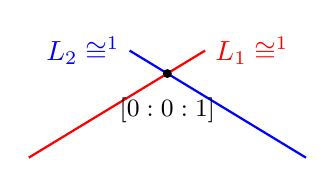
\begin{tikzpicture}[scale=0.8]
\draw[thick, red] (-2.2,-0.8) -- (0.6,0.9) node[right] {$L_1\cong\PP^1$};
\draw[thick, blue] (2.2,-0.8) -- (-0.6,0.9) node[left] {$L_2\cong\PP^1$};
\fill (0,0.535) circle (2pt);
\node[below] at (0,0.3) {\small $[0:0:1]$};
\end{tikzpicture}
\end{center}

\exsol{prob:ch15-7-2}
チャート $(u,y,\lambda)$ では $x = -u\lambda$、$v = -y\lambda$（$xy = -u\lambda y = uv$ を満たす）。微分すると
\[
dx = -\lambda\,du - u\,d\lambda,\qquad dv = -\lambda\,dy - y\,d\lambda .
\]
$du\wedge du = 0$、$d\lambda\wedge d\lambda = 0$ に注意して
\[
dx\wedge du\wedge dv = (-u\,d\lambda)\wedge du\wedge(-\lambda\,dy - y\,d\lambda) = u\lambda\,d\lambda\wedge du\wedge dy = u\lambda\,du\wedge dy\wedge d\lambda .
\]
（$d\lambda\wedge du\wedge dy\to du\wedge dy\wedge d\lambda$ は巡回置換で符号は $+$。）$x = -u\lambda$ で割ると
\[
\Omega = \frac{dx\wedge du\wedge dv}{x} = -\,du\wedge dy\wedge d\lambda .
\]
この式は最初 $x\neq0$（$u\lambda\neq0$）の部分で得られたが、右辺はチャート $\C^3_{(u,y,\lambda)}$ 全体で正則かつ至る所非零である。
特に例外曲線（$\mathcal C$ の原点の逆像）はこのチャートでは $\{u = y = 0\}$（$\lambda$ が $\PP^1$ の座標）であり、その上でも $\Omega\ne0$。

例外曲線の残りの 1 点 $\lambda = \infty$ はもう一方のチャート $\lambda_1 = \mu$、$\lambda_2 = 1$ で見る。条件 $x\mu + u = 0$、$v\mu + y = 0$ より $u = -x\mu$、$y = -v\mu$ で座標は $(x,v,\mu)$。このとき
\[
dx\wedge du\wedge dv = dx\wedge(-\mu\,dx - x\,d\mu)\wedge dv = -x\,dx\wedge d\mu\wedge dv,\qquad
\Omega = -\,dx\wedge d\mu\wedge dv = dx\wedge dv\wedge d\mu ,
\]
これも至る所正則かつ非零である（例外曲線は $\{x = v = 0\}$）。2 つのチャートは $\hat{\mathcal C}$ を覆い、$\Omega$ は稠密開集合 $\{x\neq0\}$ 上で一致する同じ形式の延長なので、
$\Omega$ は $\hat{\mathcal C}$ 上の至る所零にならない正則 3 形式に延長される。したがって $K_{\hat{\mathcal C}}\cong\OO_{\hat{\mathcal C}}$ で、小解消は crepant である。

\exsol{prob:ch15-8-1}
標準埋め込みでは $n_{\mathbf{27}} = h^{2,1}$、$n_{\overline{\mathbf{27}}} = h^{1,1}$、正味の世代数は $N_{\rm gen} = |h^{2,1}-h^{1,1}| = |\chi|/2$ である（15.8.5節）。各 Hodge 数は本文で計算した。
\begin{center}
\renewcommand{\arraystretch}{1.3}
\begin{tabular}{c|c|c|c|c|c}
& $X$ & $(h^{1,1},h^{2,1})$ & $\chi$ & $n_{\mathbf{27}}$, $n_{\overline{\mathbf{27}}}$ & $N_{\rm gen}$\\ \hline
(a) & $\PP^4[5]$ & $(1,101)$ & $-200$ & $101$, $1$ & $100$\\
(b) & $\PP^5[3,3]$ & $(1,73)$ & $-144$ & $73$, $1$ & $72$\\
(c) & $\PP^2\times\PP^2[(3,3)]$ & $(2,83)$ & $-162$ & $83$, $2$ & $81$\\
(d) & $\widetilde{\PP(1,1,2,2,2)[8]}$ & $(2,86)$ & $-168$ & $86$, $2$ & $84$\\
\end{tabular}
\end{center}
（(a) は 15.5.5節、(b) は例\ref{ex:ch15-33}、(c) は例\ref{ex:ch15-bicubic}、(d) は例\ref{ex:ch15-P11222}・例\ref{ex:ch15-P11222res}。）
いずれも $h^{2,1}>h^{1,1}$ で $\mathbf{27}$ が余る。どれも 3 世代からは程遠い。

(d) の $\chi = -168$ は次のように確かめられる。解消 $\tilde X$ は $[x_0:x_1]$ への射影により $\PP^1$ 上のファイブレーションになる（$x_0 = x_1 = 0$ の曲線 $C$ を blow-up したことで写像が至る所定義される）。
$x_1 = tx_0$ のファイバーは $\PP(1,2,2,2)\cong\PP^3$（座標 $(x_0^2,x_2,x_3,x_4)$）の 4 次曲面 $(1+t^8)y^4 + x_2^4+x_3^4+x_4^4 = 0$（$y = x_0^2$）であり、$1+t^8\ne0$ なら非特異な K3 曲面（$\chi = 24$）、
$1+t^8 = 0$ の 8 個のファイバーは平面 4 次曲線 $C$（種数 3、$\chi(C) = -4$）上の錐で $\chi = 1 + \chi(C) = -3$ である（$t = \infty$ のファイバーも非特異）。よって
\[
\chi(\tilde X) = \chi(\PP^1)\cdot24 + 8\cdot(-3-24) = 48 - 216 = -168 ,
\]
$h^{1,1} = 2$ と合わせて $h^{2,1} = 2+84 = 86$ となり、本文の値と一致する。
（係数の数え上げでは重み付き次数 8 の単項式 $105$ 個から $1 + (22-1) = 22$ を引いた $83$ しか得られない。残りの $3 = g(C)$ 個は多項式の変形として現れない複素構造変形である。）

\exsol{prob:ch15-8-2}
$SU(4)\supset SU(3)$ で $\mathbf4 = \mathbf3\oplus\mathbf1$、$\bar{\mathbf4} = \bar{\mathbf3}\oplus\mathbf1$ だから
\[
\mathbf{16} = (\mathbf2,\mathbf3)\oplus(\mathbf2,\mathbf1)\oplus(\bar{\mathbf2},\bar{\mathbf3})\oplus(\bar{\mathbf2},\mathbf1).
\]
$(\mathbf 2,\mathbf4)$ は複素 8 次元、すなわち実 16 成分で、Majorana 条件は $(\bar{\mathbf2},\bar{\mathbf4})$ 成分がその複素共役であることを言う。
内部空間 $X$ 上で平行（$\nabla_m\eta = 0$）なスピノルはホロノミー群 $\mathrm{Hol}\subset SU(4)$ の不変元と一対一に対応する（本文の基本原理）。$\mathrm{Hol} = SU(3)$ のとき $\mathbf4$ の不変部分は $\mathbf1$ のみなので、保たれる超電荷は
$(\mathbf2,\mathbf1)\oplus(\bar{\mathbf2},\mathbf1)$、すなわち 4 次元の Weyl スピノル 1 個とその共役（複素 2 成分 $=$ 実 4 成分）である。
よって 16 個の超電荷のうち 4 個が残り、これは 4 次元 $\mathcal N = 1$（$Q_\alpha$、$\bar Q_{\dot\alpha}$ が 1 組）である。

\begin{itemize}
\item $T^6$（$\mathrm{Hol} = \{1\}$）：$\mathbf4$ 全体が不変で、$(\mathbf2,\mathbf4)\oplus(\bar{\mathbf2},\bar{\mathbf4})$ のすべて、すなわち 16 個が残る。4 次元 Weyl スピノル 4 個で $\mathcal N = 4$。
\item $K3\times T^2$（$\mathrm{Hol} = SU(2)$）：$SU(2)\subset SU(3)$ は $T_X = T_{K3}\oplus T_{T^2}$ の第 1 成分 $\C^2$ に作用するので $\mathbf3 = \mathbf2\oplus\mathbf1$、したがって $\mathbf4 = \mathbf2\oplus\mathbf1\oplus\mathbf1$ で不変部分は 2 次元。
残る超電荷は $2\times(\mathbf2,\mathbf1)\oplus$（共役）で $8$ 個、4 次元 $\mathcal N = 2$。
\end{itemize}
タイプ II 弦では 10 次元で $\mathbf{16}$ が 2 つ（32 個）あるので、それぞれ倍になり $T^6$、$K3\times T^2$、strict CY 3-fold で 4 次元 $\mathcal N = 8,4,2$ となる（15.8.4節の表と一致）。
